\documentclass[12pt]{article}
\usepackage[utf8]{inputenc}
\usepackage{amsmath, amssymb}
\usepackage{amsthm}

% Define proposition environment
\newtheorem*{proposition}{Proposition}
\usepackage{geometry}
\usepackage{hyperref}
\hypersetup{
    colorlinks=true,       % false: boxed links; true: colored links
    linkcolor=black,       % color of internal links (e.g., sections, table of contents)
    citecolor=black,       % color of citation links
    filecolor=black,       % color of file links
    urlcolor=black         % color of external links
}
\usepackage{graphicx}
\usepackage{subcaption}
\usepackage{enumitem}
\usepackage{fancyhdr}
\usepackage{xcolor} 
\usepackage{algorithm}
\usepackage{algpseudocode}

\usepackage[most]{tcolorbox}

\newtcolorbox{defbox}[1][]{%
  enhanced,
  colback=white,
  colframe=black,
  fonttitle=\bfseries,
  title=#1,
  coltitle=black,
  attach boxed title to top left={
    xshift=0.5cm,
    yshift=-2mm,
  },
  boxed title style={
    colframe=white,
    colback=white,
    sharp corners=south,
    boxrule=0pt,
    top=0pt,
    bottom=0pt, 
    width=0.5cm,
    height=0.5cm,
  }
}

% Page layout
\geometry{a4paper, margin=1in}
\pagestyle{fancy}
\fancyhf{}
\setlength{\headheight}{27.05003pt} % Increased to avoid fancyhdr warning
\addtolength{\topmargin}{-12.05003pt} % Optional: adjust top margin as suggested
\fancyhead[L]{\leftmark}
\fancyhead[R]{\thepage}
\renewcommand{\baselinestretch}{1.2}

\newcommand{\uSigma}{\underline\Sigma}
\newcommand{\usigma}{\underline\sigma}
\newcommand{\tr}{\triangleright}
\newcommand{\tl}{\triangleleft}
\newcommand{\blank}{\sqcup}
\newcommand{\ra}{\rightarrow}
\newcommand{\la}{\leftarrow}
\newcommand{\NP}{\textsc{NP }}
\newcommand{\coNP}{co\textsc{NP }}
\newcommand{\C}{\textsc{C}}
\newcommand{\coC}{co\textsc{C}}
\newcommand{\dquote}[1]{``#1''}
% Title and Author
\title{Computational Complexity}
\author{Manuel Mignogna}
\date{\today}

\begin{document}

\maketitle
\tableofcontents
\newpage

\section{Turing Machine}
\subsection{Definition}
Formally, a Turing Machine is a quadruple $M=(K,\Sigma,\delta,s)$ where: $K$ is a finite set of states, $s\in K$ is the initial state, $\Sigma$ is a finite set of symbols (we say that $\Sigma$ is the alphabet of $M$), $\blank\in\Sigma$ is a special symbol called the blank symbol, $\tr\in\Sigma$ is a special symbol called the first symbol, $\delta$ is a transition function $$\delta : K\times\Sigma
 \to (K\cup\{h,\text{"yes"},\text{"no"}\})\times\Sigma\times\{\la,\ra,-\}$$
We assume that $h$ (the halting state), "yes" (the accepting state), and "no" (the rejecting state), and the cursor directions $\la$ for "left", $\ra$ for "right", and $-$ for "stay", are not in $K\cup\Sigma$.
The function $\delta$ is the "program" of the machine. It specifies, for each combination of current state $q\in K$ and current symbol $\sigma\in\Sigma$, a triple $$\delta(q,\sigma)= (p,\rho,D)$$ where: $p$ is the next state, $\rho$ is the symbol to be written on $\sigma$ and $D\in\{\la,\ra,-\}$  is the direction in which the cursor will move. For $\tr$ we require that, if for states $q$ and $p$, $\delta(q,\tr)=(p,\rho,D)$, then $\rho=\tr$ and $D=\ra$. That is, $\tr$ always directs the cursor to the right, and is never erased.

\subsection{Program execution}
How is the program to start? Initially, the state is $s$. The string is initialized to a $\tr$, followed by a finitely long string $x \in (\Sigma - \{\blank\})^*$. We say that $x$ is the input of the Turing machine. The cursor is pointing to the first symbol, always a $\tr$.

From this initial configuration, the machine takes a step according to $\delta$, changing its state, printing a symbol, and moving the cursor; then it takes another step, and another. Note that, by our requirement on $\delta(p, \tr)$, the string will always start with a $\tr$, and thus the cursor will never "fall off" the left end of the string.

Although the cursor will never fall off the left end, it will often wander off the right end of the string. In this case, we think that the cursor scans a $\blank$, which of course may be overwritten immediately. This is how the string becomes longer—a necessary feature if we wish our machines to perform general computation. The string never becomes shorter.

Since $\delta$ is a completely specified function, and the cursor never falls off the left end, there is only one reason why the machine cannot continue: One of the three halting states $h$, "yes", and "no" has been reached. If this happens, we say that the machine has halted. Furthermore, if state "yes" has been reached, we say the machine accepts its input; if "no" has been reached, then it rejects its input. If a machine halts on input $x$, we can define the output of the machine $M$ on $x$, denoted $M(x)$. If $M$ accepts or rejects $x$, then $M(x) = \text{"yes"}$ or $\text{"no"}$, respectively. Otherwise, if $h$ is reached, then the output is the string of $M$ at the time of halting. Since the computation has gone on for finitely many steps, the string consists of a $\tr$, followed by a finite string $y$, whose last symbol is not a $\blank$, possibly followed by a string of $\blank$s ($y$ could be empty). 

We consider string $y$ to be the output of the computation, and write $M(x) = y$. Naturally, it is possible that $M$ will never halt on input $x$. If this is the case, we write $M(x) = \nearrow$.

\subsection{Configuration}
We can define the operation of a Turing machine formally using the notion of a \textit{configuration}. Intuitively, a configuration contains a complete description of the current state of the computation. Formally, a configuration of $M$ is a triple $(q, w, u)$, where $q \in K$ is a state, and $w, u$ are strings in $\Sigma^*$. 

$w$ is the string to the left of the cursor, including the symbol scanned by the cursor, and $u$ is the string to the right of the cursor, possibly empty. $q$ is the current state.
\subsubsection{Configuration Yields}
We say that configuration $(q, w, u)$ \textit{yields} configuration $(q', w', u')$ in one step, denoted 
$$(q, w, u) \xrightarrow{M} (q', w', u'),$$ 
intuitively if a step of the machine from configuration $(q, w, u)$ results in configuration $(q', w', u')$. Formally, it means that the following holds. 

First, let $\sigma$ be the last symbol of $w$, and suppose that $\delta(q, \sigma) = (p, \rho, D)$. Then we must have that $q' = p$. We have three cases:
If $D = \ra$, then $w'$ is $w$ with its last symbol (which was a $\sigma$) replaced by $\rho$, and the first symbol of $u$ appended to it ($\sqcup$ if $u$ is the empty string); $u'$ is $u$ with the first symbol removed (or, if $u$ was the empty string, $u'$ remains empty).
If $D = \la$, then $w'$ is $w$ with $\sigma$ omitted from its end, and $u'$ is $u$ with $\rho$ attached in the beginning.
Finally, if $D = -$, then $w'$ is $w$ with the ending $\sigma$ replaced by $\rho$, and $u' = u$.

Once we defined the relationship of \textit{yields in one step} among configurations, we can define \textit{yields} to be its transitive closure. That is, we say that configuration $(q, w, u)$ \textit{yields} configuration $(q', w', u')$ in $k$ steps, denoted 
$$(q, w, u) \xrightarrow{M^k} (w', q', u'),$$ 
where $k \geq 0$ is an integer, if there are configurations $(q_i, w_i, u_i)$, $i = 1, \ldots, k + 1$, such that $(q_i, w_i, u_i) \xrightarrow{M} (q_{i+1}, w_{i+1}, u_{i+1})$ for $i = 1, \ldots, k$, $(q_1, w_1, u_1) = (q, w, u)$, and $(q_{k+1}, w_{k+1}, u_{k+1}) = (q', w', u')$. 

Finally, we say that configuration $(q, w, u)$ \textit{yields} configuration $(q', w', u')$, denoted 
$$(q, w, u) \xrightarrow{M^*} (q', w', u'),$$ 
if there is a $k \geq 0$ such that $(q, w, u) \xrightarrow{M^k} (q', w', u')$. 

\subsection{Turing Machine for palindromes}
\begin{figure}[ht]
\centering
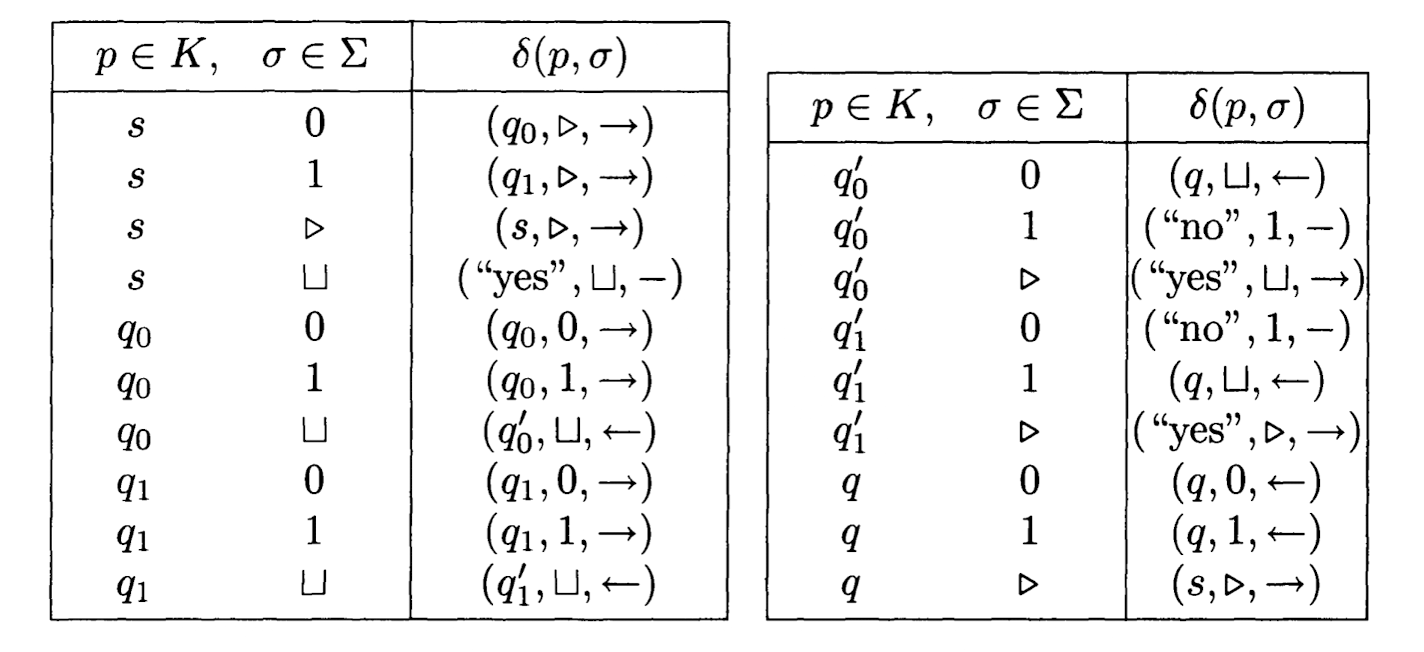
\includegraphics[width=1\textwidth]{img/TM_palindrom.png}
\end{figure}
The machine works as follows: In state $s$, it searches its string for the first symbol of the input. When it finds it, it makes it into a $\tr$ (thus effectively moving the left end of the string inward) and remembers it in its state. By this, we mean that $M$ enters state $q_0$ if the first symbol is a $0$, and state $q_1$ if it is a $1$ (this important capability of Turing machines to remember finite information in their state will be used over and over). $M$ then moves to the right until the first $\sqcup$ is met, and then once to the left to scan the last symbol of the input (now $M$ is in state $q_0'$ or $q_1'$, still remembering the first symbol). If this last symbol agrees with the one remembered, it is replaced with a $\sqcup$ (so that the string implodes on the right as well). Then the rightmost $\tr$ is found using a new state $q$, and then the process is repeated. Notice that, as the two boundaries of the string (a $\tr$ on the left, a $\sqcup$ on the right) have "marched inwards," the string left is precisely the string that remains to be shown a palindrome. If at some point the last symbol is different from the first symbol as remembered by the machine, then the string is not a palindrome, and we reach state "no". If we end up with the empty string (or we fail to find the last symbol, which means that the string was a single symbol) we express our approval by "yes".
\\
On input $0010$, the following configurations, among others, will be yielded:
$$
(s, \tr, 0010) \xrightarrow{M^5} (q_0, \tr 010 \sqcup, \epsilon) \xrightarrow{M} (q_0', \tr 010, \sqcup) \xrightarrow{M} (q, \tr 01, 01 \sqcup) \xrightarrow{M} (s, \tr 0, 1 \sqcup) \xrightarrow{M}$$
$$ (q_0, \tr \tr, 1 \sqcup) \xrightarrow{M^2} (q_0, \tr \tr 1, \sqcup) \xrightarrow{M} (q_0', \tr \tr, \sqcup) \xrightarrow{M} (\text{"no"}, \tr \tr \sqcup, \sqcup).
$$
\\
On input $101$, the computation is as follows:
$$
(s, \tr, 101) \xrightarrow{M^3} (q_1, \tr 01, \sqcup) \xrightarrow{M} (q, \tr 0, 01 \sqcup) \xrightarrow{M} (s, \tr 0, \sqcup) \xrightarrow{M} $$
$$(q_0, \tr \tr, \sqcup) \xrightarrow{M} (q_0', \tr \tr, \sqcup) \xrightarrow{M} (\text{"yes"}, \tr \tr, \sqcup).
$$
\\
On input $\epsilon$ (the shortest palindrome in the world), here is the computation:
$$
(s, \tr, \epsilon) \xrightarrow{M} (s, \tr \sqcup, \epsilon) \xrightarrow{M} (\text{"yes"}, \tr \sqcup, \epsilon).
$$

\subsection{Turing Machines as Algorithms}
\begin{defbox}[Recursive Language]
Let $L \subset (\Sigma - \{\sqcup\})^*$ be a language, that is, a set of strings of symbols. Let $M$ be a Turing machine such that, for any string $x \in (\Sigma - \{\sqcup\})^*$:
If $x \in L$, then $M(x) = \text{"yes"}$ (that is, $M$ on input $x$ halts at the "yes" state),
and if $x \notin L$, then $M(x) = \text{"no"}$.

Then we say that $M$ \textit{decides} $L$. If $L$ is decided by some Turing machine $M$, then $L$ is called a \textit{recursive language}. For example, palindromes over $\{0,1\}^*$ constitute a recursive language decided by machine $M$ defined previously.

We say that $M$ simply \textit{accepts} $L$ whenever, for any string $x \in (\Sigma - \{\sqcup\})^*$:
If $x \in L$, then $M(x) = \text{"yes"}$;
however, if $x \notin L$, then $M(x) = \nearrow$.

If $L$ is accepted by some Turing machine $M$, then $L$ is called \textit{recursively enumerable}.
\end{defbox}

\begin{defbox}
\begin{proposition}
    If $L$ is recursive, then it is recursively enumerable.
\end{proposition}
\begin{proof}
    Suppose that there is a Turing machine $M$ that decides $L$. We shall construct from $M$ a Turing machine $M'$ that \textit{accepts} $L$, as follows: $M'$ behaves exactly like $M$. Except that, whenever $M$ is about to halt and enter state "no", $M'$ moves to the right forever, and never halts.
\end{proof}
\end{defbox}

\begin{defbox}[Recursive Function]
     We shall not only deal with the decision and acceptance of languages, but also occasionally with the \textit{computation of string functions}. Suppose that $f$ is a function from $(\Sigma - \{\sqcup\})^*$ to $\Sigma^*$, and let $M$ be a Turing machine with alphabet $\Sigma$. We say that $M$ \textit{computes} $f$ if, for any string $x \in (\Sigma - \{\sqcup\})^*$, $M(x) = f(x)$. If such an $M$ exists, $f$ is called a \textit{recursive function}.
\end{defbox}

\subsection{Problems encoding}
Thus, Turing machines can be thought of as algorithms for solving string-related problems. But how about our original project, to develop a notation for algorithms capable of attacking problems like those identified in the previous chapter, whose instances are mathematical objects such as graphs, networks, and numbers? 

To solve such a problem by a Turing machine, we must decide how to \textit{represent by a string} an instance of the problem. Once we have fixed this representation, an algorithm for a decision problem is simply a Turing machine that decides the corresponding language. That is, it accepts if the input represents a "yes" instance of the problem, and rejects otherwise. Similarly, problems that require more complex output, such as \textsc{Max Flow}, are solved by the Turing machine that computes the appropriate function from strings to strings (where the output is similarly represented as a string).

It should be clear that this proposal is quite general. Any "finite" mathematical object of interest can be represented by a finite string over an appropriate alphabet. For example:
- Elements of finite sets, such as the nodes of a graph, can be represented as integers in binary.
- Pairs and $k$-tuples of simpler mathematical objects are represented by using parentheses and commas.
- Finite sets of simpler objects are represented by using set brackets, and so on.

Or, perhaps, a graph can be represented by its \textit{adjacency matrix}, which in turn can be arranged as a string, with rows separated by some special symbol such as `;`.

There is a wide range of acceptable representations of integers, finite sets, graphs, and other such elementary objects. They may differ a lot in form and succinctness. \textit{However, all acceptable encodings are related polynomially.} That is, if $A$ and $B$ are both "reasonable" representations of the same set of instances, and representation $A$ of an instance is a string with $n$ symbols, then representation $B$ of the same instance has length at most $p(n)$, for some polynomial $p$. For example, representing a graph with no isolated points by its adjacency matrix is at most quadratically more wasteful than representing it by an adjacency list.

Representing numbers in unary, instead of binary or decimal, is about the only possible slip in this regard. Obviously, the unary representation (in which, for example, number 14 is "IIIIIIIIIIIIII") requires exponentially more symbols than the binary representation. As a result, the complexity of an algorithm, measured as a function of the length of the input of the Turing machine, may seem deceptively favorable.

\newpage
\section{Multi-tape Turing Machine}
\begin{defbox}[Definition of Multi-tape Turing Machine]
    A \textit{$k$-string Turing machine}, where $k \geq 1$ is an integer, is a quadruple $M = (K, \Sigma, \delta, s)$, where $K$, $\Sigma$, and $s$ are exactly as in ordinary Turing machines. $\delta$ is a program that must reflect the complexities of multiple strings. Intuitively, $\delta$ decides the next state as before, but also decides \textit{for each string} the symbol overwritten, and the direction of cursor motion by looking at the current state and the current symbol \textit{at each string}. 
    
    Formally, $\delta$ is a function from $K \times \Sigma^k$ to 
    \[
    (K \cup \{h, \text{"yes"}, \text{"no"}\}) \times (\Sigma \times \{\leftarrow, \rightarrow, -\})^k.
    \]
    Intuitively, $\delta(q, \sigma_1, \ldots, \sigma_k) = (p, \rho_1, D_1, \ldots, \rho_k, D_k)$ means that, if $M$ is in state $q$, the cursor of the first string is scanning a $\sigma_1$, that of the second a $\sigma_2$, and so on, then the next state will be $p$, the first cursor will write $\rho_1$ and move in the direction indicated by $D_1$, and so on for the other cursors. 
    
    $\tr$ still cannot be overwritten or passed on to the left: If $\sigma_i = \tr$, then $\rho_i = \tr$ and $D_i = \rightarrow$. Initially, all strings start with a $\tr$; the first string also contains the input. The outcome of the computation of a $k$-string machine $M$ on input $x$ is as with ordinary machines, with one difference: In the case of machines that compute functions, the output can be read from the \textit{last ($k$th) string} when the machine halts.
\end{defbox}

\subsection{2-tape Turing Machine for palindromes}
  \begin{figure}[ht]
    \centering
    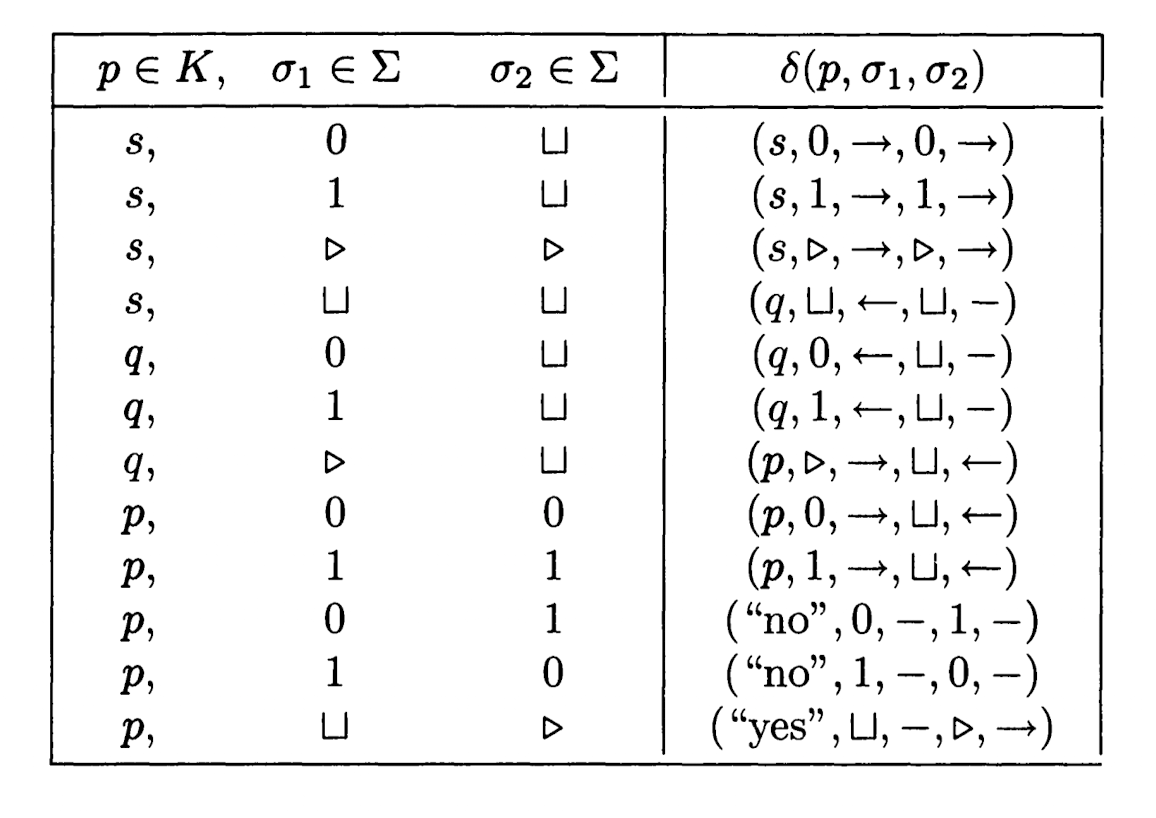
\includegraphics[width=0.8\textwidth]{img/2kTM_palindrom.png}
  \end{figure}
  We can decide palindromes more efficiently with a 2-tape Turing machine. This machine starts by copying its input in the second string. Next,it positions the cursor of the first string at the first symbol of the input, and the cursor of the second string at the last symbol of the copy. Then, it moves the two cursors in opposite directions, checking that the two symbols under them are identical at all steps, at the same time erasing the copy.
  

\subsection{Configuration of a Multi-tape Turing Machine}

A configuration of a $k$-string Turing machine is defined analogously with ordinary Turing machines. It is a $(2k + 1)$-tuple $(q, w_1, u_1, \ldots, w_k, u_k)$, where $q$ is the current state, the $i$th string reads $w_i u_i$, and the last symbol of $w_i$ is holding the $i$th cursor. We say that 
$(q, w_1, u_1, \ldots, w_k, u_k) \text{ yields in one step } (q', w_1', u_1', \ldots, w_k', u_k')$ denoted 
$$(q, w_1, u_1, \ldots, w_k, u_k) \xrightarrow{M} (q', w_1', u_1', \ldots, w_k', u_k')$$
if the following is true. 

First, suppose that $\sigma_i$ is the last symbol of $w_i$, for $i = 1, \ldots, k$, and suppose that 
\[
\delta(q, \sigma_1, \ldots, \sigma_k) = (p, \rho_1, D_1, \ldots, \rho_k, D_k).
\]
Then, for $i = 1, \ldots, k$ we have the following:
- If $D_i = \rightarrow$, then $w_i'$ is $w_i$ with its last symbol (which was a $\sigma_i$) replaced by $\rho_i$, and the first symbol of $u_i$ appended to it ($\sqcup$ if $u_i$ is the empty string); $u_i'$ is $u_i$ with the first symbol removed (or, if $u_i$ was the empty string, $u_i'$ remains empty).
- If $D_i = \leftarrow$, then $w_i'$ is $w_i$ with $\sigma_i$ omitted from its end, and $u_i'$ is $u_i$ with $\rho_i$ attached in the beginning.
- Finally, if $D_i = -$, then $w_i'$ is $w_i$ with the ending $\sigma_i$ replaced by $\rho_i$, and $u_i' = u_i$.

In other words, the conditions for yielding in single-string Turing machines must hold at each string. The relations ``yields in $n$ steps'' and plain ``yields'' are defined analogously with ordinary Turing machines.

A $k$-string Turing machine starts its computation on input $x$ with the configuration 
\[
(s, \tr, x, \tr, \epsilon, \ldots, \tr, \epsilon);
\]
that is, the input is the first string, and all strings start with an $\tr$. If 
\[
(s, \tr, x, \tr, \epsilon, \ldots, \tr, \epsilon) \xrightarrow{M^*} (\text{"yes"}, w_1, u_1, \ldots, w_k, u_k),
\]
for some strings $w_1, u_1, \ldots, u_k$, then we say that $M(x) = \text{"yes"}$; if 
\[
(s, \tr, x, \tr, \epsilon, \ldots, \tr, \epsilon) \xrightarrow{M^*} (\text{"no"}, w_1, u_1, \ldots, w_k, u_k),
\]
then we say that $M(x) = \text{"no"}$. Finally, if the machine halts at configuration $(h, w_1, u_1, \ldots, w_k, u_k)$, then $M(x) = y$, where $y$ is $w_k u_k$ with the leading $\triangleright$ and all trailing $\sqcup$s removed. That is, if $M$ halts at state $h$ (the state that signals the output is ready), the output of the computation is contained in the last string. 

Notice that, by these conventions, an ordinary Turing machine is indeed a $k$-string Turing machine with $k = 1$. Also, once the meaning of $M(x)$ has been defined, we can simply extend to multistream Turing machines the definitions of function computation, and language decision and acceptance of the previous section.

\subsection{TIME class}
\begin{defbox}[TIME class]
  We shall use the multistreaming model of the Turing machine as the basis of our notion of the time expended by Turing machine computations (for space we shall need a minor modification introduced later in this chapter).

  If for a $k$-string Turing machine $M$ and input $x$ we have 
  \[
  (s, \triangleright, x, \triangleright, \epsilon, \ldots, \triangleright, \epsilon) \xrightarrow{M^t} (H, w_1, u_1, \ldots, w_k, u_k)
  \]
  for some $H \in \{h, \text{"yes"}, \text{"no"}\}$, then the time required by $M$ on input $x$ is $t$. That is, the time required is simply the number of steps to halting. If $M(x) = \nearrow$, then the time required by $M$ on $x$ is thought to be $\infty$ (this will rarely be the case in this book).
  
  Defining the time requirements of a single computation is only the start. What we really need is a notion that reflects our interest in solving any instance of a problem, instead of isolated instances. Recall that the performance of algorithms in the previous chapter was characterized by the amount of time and space required on instances of ``size'' $n$, when these amounts were expressed as a function of $n$. For graphs, we used the number of nodes as a measure of ``size.'' For strings, the natural measure of size is the length of the string. Accordingly, let $f$ be a function from the nonnegative integers to the nonnegative integers. We say that machine $M$ operates within time $f(n)$ if, for any input string $x$, the time required by $M$ on $x$ is at most $f(|x|)$ (by $|x|$ we denote the \textit{length} of string $x$). Function $f(n)$ is a time bound for $M$.
  
  Suppose now that a language $L \subset (\Sigma - \{\sqcup\})^*$ is decided by a multistream Turing machine operating in time $f(n)$. We say that $L \in \text{TIME}(f(n))$. That is, $\text{TIME}(f(n))$ is a set of languages. It contains exactly those languages that can be decided by Turing machines with multiple strings operating within the time bound $f(n)$.
  \textbf{TIME}$(f(n))$ is what we call a \textit{complexity class}. It is a set of languages (hopefully, including many that represent important decision problems). The property shared by these languages is that they can all be decided within some specified bound on some aspect of their performance (time, soon space, and later others). Complexity classes, and their relationship with the problems they contain, are the main objects of study in this book.
\end{defbox}


\subsection{\textcolor{red}{Speed up Multi-tape}}

\begin{defbox}[\textcolor{red}{Theorem (Speed up Multi-tape)}]
  Given any $k$-string Turing Machine $M$ operating within time $f(n)$, we can construct single string Turing Machine $M'$ operating within time $O(f(n)^2)$ and such that, for any input $x$, $M(x)=M'(x)$
\end{defbox}
\begin{proof}
Suppose that $M=(K,\Sigma,\delta,s)$; We shall describe $M'=(K',\Sigma',\delta',s)$. 
  $M'$ single string must "simulate" the $k$ strings of $M$. 
  
  One way to do this would be to maintain in $M'$'s string the concatenation of the strings of $M$ (without, of course the $\tr_s$ that would come in the way of going back and forth in the string). We must also "remember" the position of each cursor, as well as the current right end of each string.
  To accomplish all this, we let $$\Sigma'=\Sigma\cup\uSigma\cup\{\tr',\tl,\tl'\}$$ Here $\uSigma=\{\usigma:\sigma\in\Sigma\}$ is a set of cursor versions of the symbol in $\Sigma$.
  $\tr'$ is a new version of $\tr$ which can be passed over to the left, and $\tl$ marks the right end of a string.
  
  Thus, any configuration $(q,w_1,u_1,\dots,w_k,u_k)$ can be simulated by the configurations of $M'$ $(q,\tr,w_1'u_1\tl w_2'u_2\tl\dots w_k'u_k\tl\tl)$. Here $w_i'$ is $w_i$ with the leading $\triangleright$ replaced by $\triangleright'$, and the last symbol $\sigma_i$ by $\underline{\sigma_i}$. The last two $\triangleleft$s signal the end of $M'$'s string.

  For the simulation to begin, $M'$ has simply to shift its input one position to the right, precede it with a $\triangleright'$, and write the string 
  $ \triangleleft (\triangleright' \triangleleft)^{k-1} \triangleleft$
  after its input. This can be easily accomplished by adding to the states of $M'$ $2k + 2$ new states, whose sole purpose is to perform this writing.
  
  To simulate a move of $M$, $M'$ scans twice its string from left to right and back. In the first scan, $M'$ gathers information concerning the $k$ currently scanned symbols in $M$: They are the $k$ underlined symbols encountered. To do this ``remembering,'' $M'$ must contain new states, each of which corresponds to a particular combination of a state of $M$ and of a $k$-tuple of symbols of $M$.
  
  Based on its state at the end of the first scan, $M'$ knows what changes need to be performed on the string to reflect changes in the strings of $M$ at the move being simulated. Then $M'$ scans its string again from left to right, stopping at each underlined symbol to rewrite one or two symbols nearby, in a manner that reflects the symbols overwritten and the cursor motions of $M$ at this string during this move. These updates can be easily performed based on the information available to $M'$.

  There is however one complication: If a cursor scanning the right end of a string needs to move right, we must create space for a new symbol (a $\sqcup$). This is done by first marking the currently scanned $\lhd$ by a special mark, making it $\lhd'$, moving $M'$'s cursor all the way to the $\lhd$ on the right end, and moving all symbols one position to the right, as was done by the Turing machine in Example 2.1. When the $\lhd'$ is encountered, it is moved to the right as a simple $\lhd$, and a $\sqcup$ is overwritten in its old position. Then we go on to implement the changes in the next string of $M$.
  
  The simulation proceeds until $M$ halts. At this point, $M'$ erases all strings of $M$ except the last (so that its output is the same as that of $M$) and halts.
  
  How long does the operation of $M'$ on an input $x$ take? Since $M$ halts within time $f(|x|)$, during its operation none of its strings ever becomes longer than $f(|x|)$ (this is a very basic fact about any reasonable model of computation: It cannot waste more space than time!). Thus the total length of the string of $M'$ is never more than $k(f(|x|) + 1) + 1$ (to account for the $\lhd$s). Simulating a move thus takes at most two traversals of this string from left to right and back ($4k(f(|x|) + 1) + 4$ steps), plus at most $3k(f(|x|) + 1) + 3$ steps per each string of $M$ simulated. The total is $\mathcal{O}(k^2 f(|x|)^2)$, or, since $k$ is fixed and independent of $x$, $\mathcal{O}(f(|x|)^2)$.
\end{proof}

\subsection{Linear Speedup Theorem}
As a result of this theorem, we have that e.g. 
$$\text{if } L\in\textbf{TIME}(150n^2) \text{ then } L\in\textbf{TIME}(n^2 + n +2)$$  
From this we can conclude that, $O$ is the only significative notation for time complexity.
\begin{defbox}[Linear Speedup Theorem]
  Let $L\in\textbf{TIME}(f(n))$. Then, for any $\epsilon>0$, $L\in\textbf{TIME}(f'(n))$, where $$f'(n) = \epsilon f(n)+n+2$$ 
\end{defbox}

\subsection{Space Bounds}
At first it seems straightforward to define the space used by the computation 
\[
(s, \triangleright, \epsilon, \ldots, \triangleright, \epsilon) \xrightarrow{M^*} (H, w_1, u_1, \ldots, w_k, u_k)
\]
of a Turing machine with $k$ strings. Since the strings cannot become shorter in our model, the lengths of the final strings $w_i u_i$, $i = 1, \ldots, k$, capture the amount of storage required by each during the computation. We can either add up these lengths, or take their maximum. There are arguments in favor of both approaches, but we shall cut the discussion short by noting that the two estimates differ by at most $k$, a constant. Let us say for the time being that the space used by the machine $M$ on $x$ is 
\[
\sum_{i=1}^k |w_i u_i|.
\]
It turns out that this estimate represents a serious overcharge. Consider the following example:

\begin{tcolorbox}[colback=white, colframe=black, title=Example]
\textbf{Can we recognize palindromes in space substantially less than $n$?} 

In view of our definition of the space used by a computation, the sum of the lengths of the strings at halting, this is impossible: One of these lengths, namely that of the first string carrying the input, will always be at least $|x| + 1$.

But consider the following 3-string Turing machine that recognizes palindromes: The first string contains the input, and is never overwritten. The machine works in stages. At the $i$th stage the second string contains integer $i$ in binary. During the $i$th stage we try to identify and remember the $i$th symbol of $x$. We do this by initializing the third string to $j = 1$, and then comparing $i$ and $j$. Comparisons of the contents of the two different strings are easy to do by moving the two cursors. If $j < i$, then we increment $j$ in binary (recall the machine in Example 2.2), and advance the first cursor to the right, to inspect the next input symbol. If $i = j$ we remember in our state the currently scanned symbol of the input, we reinitialize $j$ to 1, and try to identify the $i$th from the last symbol of $x$. This is done much in the same way, with the first cursor now marching from right to left instead from left to right.

If the two symbols are unequal, we halt with ``no''. If they are equal, we increment $i$ by one, and begin the next stage. If, finally, during a stage, the alleged $i$th symbol of $x$ turns out to be a $\sqcup$, this means that $i > n$, and the input is a palindrome. We halt with a ``yes''.
\end{tcolorbox}

\textbf{What space is needed for the operation of this machine?} It seems fair to assess that the space used up by this machine is $\mathcal{O}(\log n)$. The machine surely looks at the input (computation would be impossible otherwise) \textit{but in a read-only fashion}. There is no writing on the first string. The other two strings are kept at most $\log n + 1$ long. \qed

This example leads us to the following definition: Let $k > 2$ be an integer. A \textit{$k$-string Turing machine with input and output} is an ordinary $k$-string Turing machine, with one important restriction on the program $\delta$: Whenever 
\[
\delta(q, \sigma_1, \ldots, \sigma_k) = (p, \rho_1, D_1, \ldots, \rho_k, D_k),
\]
then (a) $\rho_1 = \sigma_1$, and (b) $D_k \neq \leftarrow$. Furthermore, (c) if $\sigma_1 = \sqcup$, then $D_1 = \leftarrow$. 

Requirement (a) says that at each move, the symbol ``written'' on the first string is always the same as the old symbol, and hence the machine effectively has a read-only input string. Requirement (b) states that in the last (output) string the cursor never moves to the left, and hence the output string is effectively write-only. Finally, (c) guarantees that the cursor of the input string does not wander off into the $\sqcup$s after the end of the input. It is a useful technical requirement, but not necessary.

These restrictions lead to an accurate definition of space requirements, without ``overcharging'' the computation for reading the input and for providing output, that is, for functions involving no ``remembering'' of earlier results of the computation. With these restrictions we shall be able to study space bounds smaller than $n$. However, let us first observe that these restrictions do not change the capabilities of a Turing machine.

\begin{defbox}[Proposition]
  For any $k$-string Turing machine $M$ operating within time bound $f(n)$ there is a $(k+2)$-string Turing machine $M'$ with input and output, which operates within time bound $\mathcal{O}(f(n))$.
\end{defbox}
\begin{proof}
  Machine $M'$ starts by copying its input on the second string, and then simulating the $k$ strings of $M$ on its strings numbered 2 through $k+1$. When $M$ halts, $M'$ copies its output to the $k+2$nd string, and halts.
\end{proof} 

\begin{defbox}[Space Complexity Class]
  Suppose that, for a $k$-string Turing machine $M$ and an input $x$ 
\[
(s, \triangleright, x, \ldots, \triangleright, \epsilon) \xrightarrow{M^*} (H, w_1, u_1, \ldots, w_k, u_k),
\]
where $H \in \{h, \text{"yes"}, \text{"no"}\}$ is a halting state. Then the \textit{space required by $M$ on input $x$} is 
\[
\sum_{i=1}^k |w_i u_i|.
\]
If, however, $M$ is a machine with input and output, then the space required by $M$ on input $x$ is 
\[
\sum_{i=2}^{k-1} |w_i u_i|.
\]
Suppose now that $f$ is a function from $\mathbb{N}$ to $\mathbb{N}$. We say that \textit{Turing machine $M$ operates within space bound $f(n)$} if, for any input $x$, $M$ requires space at most $f(|x|)$.

Finally, let $L$ be a language. We say that $L$ is in the \textit{space complexity class} $\textbf{SPACE}(f(n))$ if there is a Turing machine with input and output that decides $L$ and operates within space bound $f(n)$. For example, palindromes were shown to be in the space complexity class $\textbf{SPACE}(\log n)$. This important space complexity class is usually referred to as $\mathbf{L}$.  
\end{defbox}

\begin{defbox}[Theorem]
  Let $L$ be a language in $\textbf{SPACE}(f(n))$. Then, for any $\epsilon > 0$, 
\[
L \in \textbf{SPACE}(2 + \epsilon f(n)).
\]
\end{defbox}

\section{Nondeterministic Turing Machines}
We shall now break our chain of ``reasonable'' models of computation that can simulate each other with only a polynomial loss of efficiency. We shall introduce an \textit{unrealistic} model of computation, the nondeterministic Turing machine. And we shall show that it can be simulated by our other models with an \textit{exponential} loss of efficiency.
\begin{defbox}[Nondeterministic Turing Machine]
  
  A \textit{nondeterministic Turing machine} is a quadruple $N = (K, \Sigma, \Delta, s)$, much like the ordinary Turing machine. $K$, $\Sigma$, and $s$ are as before. Reflecting the fact that a nondeterministic Turing machine does not have a single, uniquely defined next action, but a choice between several next actions, $\Delta$ is no longer a function from $K \times \Sigma$ to $(K \cup \{h, \text{``yes''}, \text{``no''}\}) \times \Sigma \times \{ \leftarrow, \rightarrow, - \}$, but instead a \textit{relation} $\Delta \subseteq (K \times \Sigma) \times [(K \cup \{h, \text{``yes''}, \text{``no''}\}) \times \Sigma \times \{ \leftarrow, \rightarrow, - \}]$. That is, for each state-symbol combination, there may be \textit{more than one} appropriate next step—or none at all.
\end{defbox}

Nondeterministic Turing machine configurations are exactly like configurations of deterministic machines, but ``yields'' is no longer a function; it is instead a \textit{relation}. We say that configuration $(q, w, u)$ of the nondeterministic Turing machine $N$ \textit{yields} configuration $(q', w', u')$ in one step, denoted
\[
(q, w, u) \stackrel{N}{\rightarrow} (q', w', u'),
\]
intuitively if there is a rule in $\Delta$ that makes this a legal transition. Formally, it means that there is a move $((q, \sigma), (q', \rho, D)) \in \Delta$ such that, either (a) $D = \rightarrow$, and $w'$ is $w$ with its last symbol (which was a $\sigma$) replaced by $\rho$, and the first symbol of $u$ appended to it ($\sqcup$ if $u$ is the empty string), and $u'$ is $u$ with the first symbol removed (or, if $u$ was the empty string, $u'$ remains empty); or (b) $D = \leftarrow$, $w'$ is $w$ with $\sigma$ omitted from its end, and $u'$ is $u$ with $\rho$ attached in the beginning; or finally, (c) $D = -$, $w'$ is $w$ with the ending $\sigma$ replaced by $\rho$, and $u' = u$. $N^k \stackrel{k}{\rightarrow}$ and $N^* \stackrel{*}{\rightarrow}$ can be defined as usual, but $N^k \stackrel{k}{\rightarrow}$ is, once more, no longer a function.

What makes nondeterministic machines so different and powerful is the very weak ``input-output behavior'' we demand of them, that is, our very liberal notion of what it means for such a machine to ``solve a problem.'' Let $L$ be a language and $N$ a nondeterministic Turing machine. We say that $N$ \textit{decides} $L$ if for any $x \in \Sigma^*$, the following is true:
\[
x\in L \iff (s, \tr, x) \stackrel{N^*}{\rightarrow} (\text{"yes"}, w, u)
\]
for some strings $w$ and $u$.

This is the crucial definition that sets nondeterministic machines apart from other models. An input is accepted if there is \textit{some} sequence of nondeterministic choices that results in ``yes.'' Other choices may result in rejection; just one accepting computation is enough. The string is rejected only if no sequence of choices can lead to acceptance.

We say that nondeterministic Turing machine $N$ decides language $L$ \textit{in time} $f(n)$, where $f$ is a function from the nonnegative integers to the nonnegative integers, if $N$ decides $L$, and, moreover for any $x \in \Sigma^*$, if 
\[
(s, \triangleright, x) \stackrel{N^k}{\rightarrow} (q, u, w),
\]
then $k \leq f(|x|)$. That is, we require that $N$, besides deciding $L$, does not have computation paths longer than $f(n)$, where $n$ is the length of the input. Thus, we charge to a nondeterministic computation an amount of time that may be considered unrealistically small. The amount of time charged is the ``depth'' of the computational activity. Obviously, the ``total computational activity'' generated can be exponentially bigger.
\begin{figure}[ht]
    \centering
    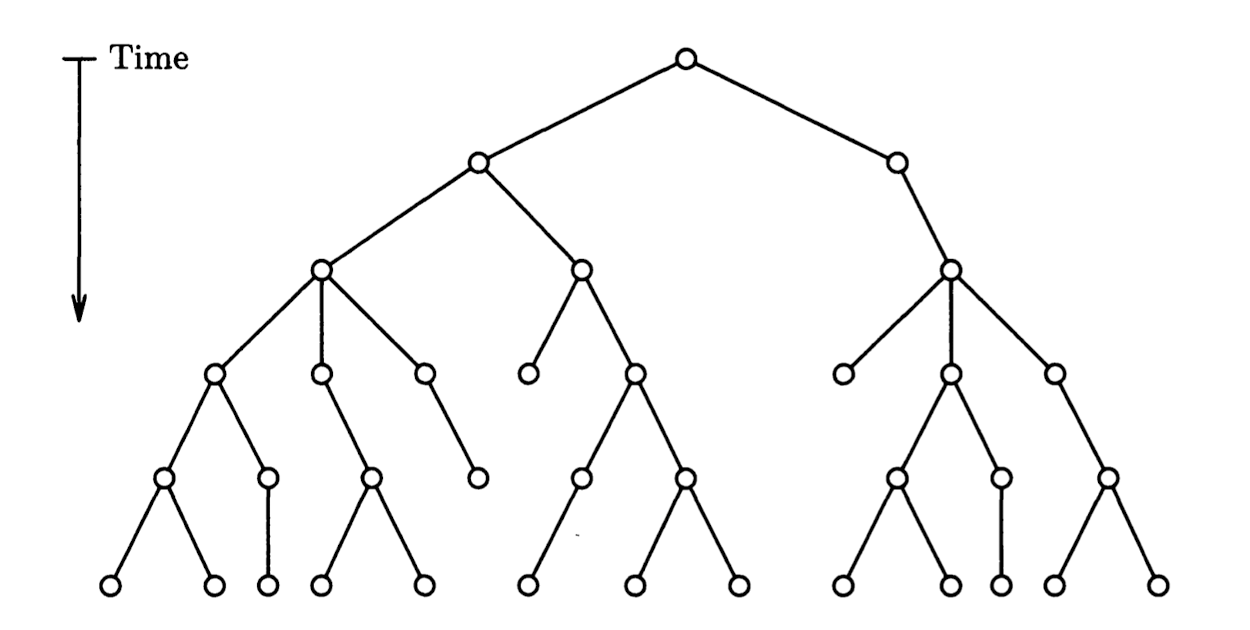
\includegraphics[width=0.8\textwidth]{img/ndc.png}
    \caption{Nondeterministic computation}
    \label{fig:nondeterministic}
\end{figure}
\\
The set of language decided by nondeterministic Turing machines within time $f$ is a new, important kind of complexity class, denoted $\textbf{NTIME}(f(n))$. A most important nondeterministic complexity class is $\textbf{NP}$, the union of all $\textbf{NTIME}(n^k)$. Notice immediately that $\textbf{P}\subseteq\textbf{NP}$; the reason is that deterministic machines from a subclass of the nondeterministic ones: They are precisely those for which the relation $\Delta$ happens to be a function.
\begin{tcolorbox}[colback=white, colframe=black, title=Example]
  Recall that we do not know whether the decision version of the traveling salesman problem, $\text{TSP (D)}$ (recall Section 1.3), is in $\textbf{P}$. However, it is easy to see that $\text{TSP (D)}$ is in $\textbf{NP}$, because it can be decided by a nondeterministic Turing machine in time $\mathcal{O}(n^2)$. This machine, on an input containing a representation of the $\text{TSP}$ instance, goes on to write an arbitrary sequence of symbols, no longer than its input. When this writing stops, the machine goes back and checks to see whether the string written is the representation of a permutation of the cities, and, if so, whether the permutation is a tour with cost $B$ or less. Both tasks can easily be carried out in $\mathcal{O}(n^2)$ time by using a second string (multistring nondeterministic Turing machines are straightforward to define; they can be simulated by single-string ones again with a quadratic slowdown). If the string indeed encodes a tour cheaper than $B$, the machine accepts; otherwise, it rejects (perhaps hoping that another choice of symbols, written at some other branch of the tree in Figure 2.9, will end up accepting).
  
  This machine indeed decides $\text{TSP (D)}$, because it accepts its input if and only if it encodes a ``yes'' instance of $\text{TSP (D)}$. If the input is a ``yes'' instance, this means that there is a tour of the cities with cost $B$ or less. Therefore, there will be a computation of this machine that ``guesses'' precisely this permutation, checks that its cost is indeed below $B$, and thus ends up accepting. It does not matter that other computations of the machine may have guessed very costly tours, or plain nonsense strings, and will therefore reject; a single accepting computation is all that is needed for the machine to accept. Conversely, if there are no tours of cost less than $B$, there is no danger that a computation will accept: All computations will discover that their guess is wrong, and will reject. Thus, according to our convention, the input will be rejected. \qed
  \end{tcolorbox}
  
  It would be remarkable if we could somehow turn this nondeterministic idea into a viable, polynomial-time algorithm for $\text{TSP (D)}$. Unfortunately, at present we know of only exponential general methods for turning a nondeterministic algorithm into a deterministic one. We describe the most obvious such method next.
\subsection{\textcolor{red}{From nondeterministic to deterministic}}
\begin{defbox}[\textcolor{red}{Theorem (from nondeterministic to deterministic)}]
  Suppose that language $L$ is decided by a nondeterministic Turing machine $N$ in time $f(n)$. Then it is decided by a 3-string deterministic Turing machine $M$ in time $\mathcal{O}(c^{f(n)})$, where $c > 1$ is some constant depending on $N$.

Notice that, using complexity class notation, we can restate this result very succinctly:
\[
\textbf{NTIME}(f(n)) \subseteq \bigcup_{c > 1} \textbf{TIME}(c^{f(n)})
\]
\end{defbox}
\begin{proof}
  Let $N = (K, \Sigma, \Delta, s)$. For each $(q, \sigma) \in K \times \Sigma$, consider the set of choices $C_{q,\sigma} = \{(q', \sigma', D) : ((q, \sigma), (q', \sigma', D)) \in \Delta\}$. $C_{q,\sigma}$ is a finite set. Let $d = \max_{q,\sigma} |C_{q,\sigma}|$ (this $d$ could be called the ``degree of nondeterminism'' of $N$), and assume that $d > 1$ (otherwise, the machine is deterministic, and there is nothing to do).

The basic idea for simulating $N$ is this: Any computation of $N$ is a sequence of nondeterministic choices. Now, any sequence of $t$ nondeterministic choices made by $N$ is essentially a sequence of $t$ integers in the range $0, 1, \ldots, d - 1$. The simulating deterministic machine $M$ considers all such sequences of choices, in order of increasing length, and simulates $N$ on each (notice that we cannot simply consider the sequences of length $f(|x|)$, where $x$ is the input, because $M$ must operate with no knowledge of the bound $f(n)$). While considering a sequence $(c_1, c_2, \ldots, c_t)$, $M$ maintains the sequence on its second string. Then $M$ simulates the actions that $N$ would have taken had $N$ taken choice $c_i$ at step $i$ for its first $t$ steps. If these choices would have led $N$ to halting with a ``yes'' (possibili earlier than $t$th step), then $M$ halts with a ``yes'' as well. Otherwise, $M$  proceeds to the next sequence of choices. Generating the next sequence is akin to calculating the next integer in $d$-ary, and can be done easily.
How can $M$ detect that $N$ rejects, with no knowledge of the bound $f(n)$? 
The solution is simple: If $M$ simulates all sequences of choice of a particular 
length $t$, and finds among them \textit{no continuing computation} (that is, all 
computations of length $t$ end with halting, presumably with ``no'' or $h$), then $M$ can 
conclude that $N$ rejects its input.

The time required by $M$ to complete the simulation is bounded from above 
by 
\[
\sum_{t=1}^{f(n)} d^t = O(d^{f(n)+1})
\]
(the number of sequences it needs to go through) times the time required to generate and consider each sequence, and this latter cost is easily seen to be $O(2^{f(n)})$.
\end{proof}
We shall also be very interested in the \textit{space} used by nondeterministic 
Turing machines. To do this correctly for space bounds smaller than linear, we 
shall need to define a \textit{nondeterministic Turing machine with input and output}. 
It is a straightforward task (which we omit) to combine the two extensions of 
Turing machines into one.

Given an $k$-string nondeterministic Turing machine with input and output 
$N = (K, \Sigma, \Delta, s)$, we say that $N$ decides language $L$ within space $f(n)$ if 
$N$ decides $L$ and, moreover, for any $x \in (\Sigma - \{\blank\})^*$, if 
\[
(s, \triangleright, x, \ldots, \triangleright, \epsilon) \xrightarrow{N^*} (q, w_1, u_1, \ldots, w_s, u_s),
\]
then 
\[
\sum_{j=2}^{s-1} |w_j u_j| \leq f(|x|).
\]
That is, we require that $N$ under no circumstances uses space in its ``scratch'' strings greater than function $f$ in the input length. Notice that our definition does not even require $N$ to halt on all computations.

\section{Proper Complexity Functions}
\begin{defbox}[Definition (Proper Complexity Function)]
  Let $f$ be a function from the nonnegative 
integers to the nonnegative integers. We say that $f$ is a \textit{proper complexity 
function} if $f$ is nondecreasing (that is, $f(n+1) \geq f(n)$ for all $n$), and furthermore 
the following is true: There is a $k$-string Turing machine $M_f = (K, \Sigma, \delta, s)$ 
\textit{with input and output} such that, for any integer $n$, and any input $x$ of length 
$n$, 
\[
(s, \triangleright, x, \triangleright, \epsilon, \ldots, \triangleright, \epsilon) 
\xrightarrow{M_f^t} 
(h, x, \triangleright, \sqcup^{j_2}, \triangleright, \sqcup^{j_3}, \ldots, 
\triangleright, \sqcup^{j_{k-1}}, \triangleright, \sqcup^{f(|x|)}),
\]
such that $t = O(n + f(n))$, and the $j_i = O(f(|x|))$ for $i = 2, \ldots, k - 1$, with $t$ and the 
$j_i$'s depending only on $n$. In other words, on input $x$, $M_f$ computes the string 
$\sqcup^{f(|x|)}$, where $\sqcup$ is a ``quasi-blank'' symbol. And, on any input $x$, $M_f$ halts after 
$O(|x| + f(|x|))$ steps and uses $O(f(|x|))$ space besides its input. \qed
\end{defbox}
Using only proper complexity functions we can standardize the behavior of Turing machines.
\begin{defbox}[Precise Turing Machines]
  A Turing Machine (of any type) is \textit{precise} if and only if there exist two proper functions $f$ and $g$ such that, for any input $x$, every computation of $M$ on $x$ halts after exactly $f(|x|)$ steps, and every tape of $M$ beside the input and the output tapes are long exactly $g(|x|)$.
  
\end{defbox}

\begin{defbox}[Theroem (Precise Solutions)]
  Let $M$ be any Turing machine. If $M$ decides a language $L$ in time or space $f(n)$, and $f$ is a proper complexity function, then there exist a precise Turing machine $M'$ that decides $L$ in time or space (respectively) $O(f(n))$.
\end{defbox}
\begin{proof}
  In all four cases (deterministic time, deterministic space, nondeterministic time, or nondeterministic space) the machine $M'$ on input $x$ starts off by simulating the machine $M_f$ associated with the proper function $f$ on $x$, using a new set of strings. After $M_f$'s computation has halted, $M$ uses the output string of $M_f$ as a ``yardstick'' of length $f(|x|)$, to guide its further computation. 

If $f(n)$ is a time bound, then $M'$ simulates $M$ on a different set of strings, \textit{using the yardstick as an ``alarm clock''}. That is, it advances its cursor on the yardstick after the simulation of each step of $M$, and halts if and only if a true blank is encountered, after precisely $f(|x|)$ steps of $M$. If $f(n)$ is a space bound, then $M'$ simulates $M$ on the quasiblanks of $M_f$'s output string. In either case, the machine is precise. 

If $M$ is nondeterministic, then precisely the same amount of time or space is used over all possible computations of $M'$ on $x$, as this amount depends only on the deterministic phase of $M'$ (the simulation of $M_f$). In both cases, the time or space is the time or space consumed by $M_f$, plus that consumed by $M$, and is therefore $\mathcal{O}(f(n))$.

In the case of space-bounded machines, the ``space yardstick'' can be used by $M'$ to also ``count'' steps in an appropriate base representing the size of the alphabet of $M$, and thus $M'$ will never indulge in a meaninglessly long computation. Thus, we can assume that space-bounded machines always halt.
\end{proof}

\subsection{\textcolor{red}{Termination of TM space bounded}}
\begin{defbox}[\textcolor{red}{Theorem (Termination of TM space bounded)}]
If $M$ decides $L$ in space $f(n)$, with $f$ being a proper function then exists a Turing machine $M'$ that decides $L$ in space $O(f(n))$ and such that every computation halts.
\end{defbox}
\begin{proof}
  If $M$ works in space $f(n)$, then the set of different configurations in which it can go through is finite. 
  Upper bounder by 
  $$c=|K|\times|\Sigma|^{f(n)}\times (f(n)+1)$$
  If $M$ makes more than $c$ steps, then it must have repeated a configuration and so it must be in a loop. If $M$ doesn't halt in at most $c$ steps we can force termination in "no".
  Proof for 1 tape: concatenates $M_f$ and a simulation of $M$. The last tape of $M_f$ is used as a yardstick. This tape will contain a cell in which we have the symbol representing the current state, it can contain $|K|$ different symbols. Then the next $f(n)$ cells will contain the symbols of $\Sigma$ (represented by an integer in base $|\Sigma|$). The last ($f(n)+1$) cells will be used as an unary representation of the cursor position.
  At every transition of $M$ we increment the counter and if in at most $c$ steps $M$ has not halted, we can force it to halt in "no".
\end{proof}

From this theorem we ca conclude that if the space is finite then the machine will halt. Another important result is that time is exponentially bigger than space. 

\section{Complexity Classes}
\[
\begin{aligned}
    &\text{TIME}(n^k) && = \bigcup_{j > 0} \text{TIME}(n^j)  &&= \textbf{P}, \\
    &\text{NTIME}(n^k) && = \bigcup_{j > 0} \text{NTIME}(n^j)  &&= \textbf{NP}, \\
    &\text{TIME}(2^{n^k}) && = \bigcup_{j > 0} \text{TIME}(2^{n^j})  &&= \textbf{EXP}, \\
    &\text{SPACE}(n^k) && = \bigcup_{j > 0} \text{SPACE}(n^j)  &&= \textbf{PSPACE}, \\
    &\text{NSPACE}(n^k) && = \bigcup_{j > 0} \text{NSPACE}(n^j) && = \textbf{NPSPACE}, \\
    &\text{SPACE}(\log n) &&&& = \textbf{L}, \\
    &\text{NSPACE}(\log n) &&&& = \textbf{NL}.
\end{aligned}
\]
\subsection{Exercises}
\begin{itemize}
  \item $TIME(n^3)\subseteq EXP$? Yes
  \item $TIME(n^3)\subseteq P$? Yes
  \item $EXP\subseteq P$? No (there is a theorem that proves it)
  \item $P\subseteq NTIME(n^k)$? Yes, because $P\subseteq NP$.
  \item $NTIME(n^k)\subseteq P$? We don't know.
  \item $NTIME(n^k)\subseteq NP$? Yes, because $NTIME(n^k)=NP$.
  \item $TIME(2^{n^2})\subseteq EXP$? Yes, because $EXP = \bigcup\limits_{k > 0} TIME(2^{n^k})$.
  \item $NTIME(n^2)\subseteq EXP$? Yes, because 
  $$NTIME(n^2)\subseteq TIME(k^{n^2})=TIME(2^{(log_2k)n^2})\subseteq TIME(2^{n^3})\subseteq EXP$$ to switch from nondeterministic to deterministic we used the theorem that says that nondeterministic Turing machines can be simulated by deterministic Turing machines with an exponential loss of efficiency.
  \item $PSPACE\subseteq SPACE(n^k)$? Yes, because $PSPACE = \bigcup\limits_{k > 0} SPACE(n^k)$.
  \item $PSPACE\subseteq NPSPACE$? Yes, because deterministic Turing machines are a subset of nondeterministic Turing machines.
  \item $SPACE(2^n)\subseteq SPACE(2^{n^2})$? Yes
  \item $SPACE(n)\subseteq NSPACE(n)$? Yes
  \item $NPSPACE\subseteq PSPACE$? Yes, (proven by Savitch corollary)
  \item $TIME(n^k)\subseteq PSPACE$? Yes, because $TIME(n^k)\subseteq SPACE(n^k) = PSPACE$, obviously if we have a Turing machine that works in time $n^k$ then it will use at most $n^k$ space.
  \item $PSPACE\subseteq EXP$? Yes, because we can upper bound time number of computations by $c= |K|\times|\Sigma|^{f(n)}\times (f(n)+1)$ which is exponential in $f(n)$.
  \item $NP\subseteq PSPACE$? Yes, because we can prove that any $NP$ problem can be solved in polynomial space.
\end{itemize}
\section{Complementary Complexity Classes}
When we first defined nondeterministic computation, we were struck by an asymmetry in the way ``yes'' and ``no'' inputs are treated. For a string to be established as a string in the language (a ``yes'' input), one successful computational path is enough. In contrast, for a string not in the language, all computational paths must be unsuccessful. 

\begin{defbox}[Complement of a Language]
  
  Let $L \subseteq \Sigma^*$ be a language. The \textit{complement} of $L$, denoted $\overline{L}$, is the language $\Sigma^* - L$, that is, the set of all strings in the appropriate alphabet that are not in $L$. We now extend this definition to decision problems. The complement of a decision problem $A$, usually called \textit{A complement}, will be defined as the decision problem whose answer is ``yes'' whenever the input is a ``no'' input of $A$, and vice versa. 
\end{defbox}
  
For example, \textit{SAT complement} is this problem: Given a Boolean expression $\phi$ in conjunctive normal form, is it \textit{unsatisfiable}? \textit{Hamilton path complement} is the following: Given a graph $G$, is it true that $G$ \textit{does not} have a Hamilton path? And so on. Notice that, strictly speaking, the languages corresponding to the problems \textit{Hamilton path} and \textit{Hamilton path complement}, for example, are not complements of one another, as their union is not $\Sigma^*$ but rather the set of all strings that encode graphs; this is of course another convenient convention with no deep consequences.

\begin{defbox}[Complementary Complexity Class]
  
  For any complexity class $C$, $\textbf{co}C$ denotes the class $\{\overline{L} : L \in C\}$. It is immediately obvious that if $C$ is a deterministic time or space complexity class, then $C = \textbf{co}C$; that is, \textit{all deterministic time and space complexity classes are closed under complement}. The reason is that any deterministic Turing machine deciding $L$ within a time or space bound can be converted to a deterministic Turing machine that decides $\overline{L}$ within the same time or space bound: The same machine with the roles of ``yes'' and ``no'' reversed. But it is an important open problem whether nondeterministic time complexity classes are close under complement. For nondeterministic space complexity classes we can prove closure under complement, but we will see that later. 
\end{defbox}
\section{The Hierarchy Theorem}
We shall assume that, although a machine may have an arbitrary alphabet, the languages of interest, and therefore the inputs $x$, contain the symbols used for encoding Turing machines (0, 1, ``('', ``;'', etc.). This is no loss of generality, since languages over different alphabets obviously have identical complexity properties, as long as these alphabets contain at least two symbols. We represent the states and the alphabet symbols of turing machines as integers:
\begin{itemize}
\item$\Sigma\rightsquigarrow\{1,\dots,|\Sigma|\}$
\item $K\rightsquigarrow\{|\Sigma|+1,\dots,|\Sigma|+|K|\}$
\item $\{\la,\ra,-,h,\text{"yes"},\text{"no"}\}\rightsquigarrow\{|\Sigma|+|K|+1,\dots,|\Sigma|+|K|+6\}$ 
\end{itemize}
Every integer is represented in binary, with strings of length $log(|\Sigma|+|K|+6)$. We denote with $\underline i$ the binary encoding of the integer $i$, with $\underline q$ the encoding of the state $q\in K$ and with $\underline\sigma$ the encoding of the symbol $\sigma\in\Sigma$.
Codifica di $(q, \sigma, q', \sigma', D) \in \Delta$:$(\underline q,\underline \sigma,\underline q',\underline \sigma',\underline D)$.
 Codifica di  $\Delta$, denotata con $\underline\Delta$:$ (\underline q_1,\underline \sigma_1,\underline q_1',\underline \sigma_1',\underline D_1), \dots, (\underline q_m,\underline \sigma_m,\underline q_m',\underline \sigma_m',\underline D_m) \quad (m = |\Delta|)$. Codifica di $M$, denotata con $\underline M$:$  |\underline\Sigma|, |\mathcal{\underline K}|,\underline \Delta$.
 
\begin{defbox}[Universla Turgin Machine]
  There exist a \textbf{universal} turing machine $U$ that given the string $\underline M;x$ can simulate $M$ on input $x$. We describe $U$ as a two tape turing machine since we know that it can be reduced to a one tape turing machine with just a quadratic slowdown. $U$ keeps the configuration of $M$ on the second tape with such a format: $(\underline{w, q, u})$ where $w$ is the left side of the string with respect to the cursor, $q$ is the state of the machine and $u$ is the right side of the string. $U$ simulates $M$ with the following steps: searches for the encoding of the current state $q$ in the second tape, then it searches in the first tape for a tuple $(q,\sigma,\dots)$ starting with the $q$ state. Then it keeps moving left on the second string until it reaches the left end of $w$ to verifies that the cursor is under the symbol $\sigma$. If this is true then it writes the new symbol $\sigma'$ in the first tape and moves the cursor according to $D$ otherwise searches for the next tuple starting with $q$ and keeps repeating these steps. If it finds an encoding error for $\underline M$ it keeps moving the cursor to the right forever (diverging).
  \end{defbox}
In this section, we prove a \textit{quantitative hierarchy result}: With sufficiently greater time allocation, Turing machines are able to perform more complex computational tasks. Predictably, our proof will employ a quantitative sort of diagonalization.

Let $f(n) \geq n$ be a proper complexity function, and define $H_f$ to be the following time-bounded version of the \textit{halting} language $H$:
\[
H_f = \{M; x \;|\; M \text{ accepts input } x \text{ after at most } f(|x|) \text{ steps}\},
\]
where $M$ in the definition of $H_f$ ranges over all descriptions of deterministic multi-string Turing machines. 

\begin{defbox}[Lemma (complexity upper bound of \texorpdfstring{$H_f$}{Hf})]
$$H_f\in TIME(f(n)^3)$$
\end{defbox}
\begin{proof}
  We shall describe a Turing machine $U_f$ with four strings, which decides $H_f$ in time $(f(n))^3$. $U_f$ is based on several machines that we have seen previously: The universal Turing machine $U$; the single-string simulator of multi-string machines; the linear speedup theorem machine that shaves constants off the time bound; and the ,machine $M_f$ that computes a "yardstick" of length precisely $f(n)$, which exists because we are assuming that $f$ is a proper complexity function. First, $U_f$ uses $M_f$ on the second part of its input, $x$, to initialize on its fourth string an appropriate ``alarm clock'' $\triangleright \sqcup^{f(|x|)}$, to be used during the simulation of $M$. (Here we assume that $M_f$ has at most four strings; if not, the number of strings of $U_f$ has to be increased accordingly.) $M_f$ operates within time $\mathcal{O}(f(|x|))$ (where the constant depends on $f$ alone, and not on $x$ or $M$). $U_f$ also copies the description of the machine $M$ to be simulated on its third string, and converts $x$ on its first string to the encoding of $\triangleright x$ (that is, it removes $\underline M$ from the first string and adds a $\tr$ at the beginning of $x$). The second string is initialized to the encoding of the initial state $s$ (that is, it replaces $(\underline{w,q,u})$ with only $\underline q$). We can also at this point check that indeed $\underline M$ is the description of a legitimate Turing machine, and reject if it is not (this requires linear time using two strings). The total time required so far is $\mathcal{O}(f(|x|) + n) = \mathcal{O}(f(n))$ where $n$ is the size of the input $\underline M;x$.

  The main operation of $U_f$ starts after this initial stage. Like the $U$ we defined before (universal turing machine), $U_f$ simulates one-by-one the steps of $M$ on input $x$. The simulation is confined in the first string, where the encodings of the contents of all strings of $M$ are kept. Each step of $M$ is simulated by two successive scans of the first string of $U_f$. During the first scan, $U_f$ collects all relevant information concerning the currently scanned symbols of $M$, and writes this information on the second string. The second string also contains the encoding of the current state. $U_f$ then matches the contents of the second string with those of the third (containing the description of $M$) to find the appropriate transition of $M$. $U_f$ goes on to perform the appropriate changes to its first string, in a second pass. It also advances its ``alarm clock'' by one.
  
  $U_f$ simulates each step of $M$ in time $\mathcal{O}(\ell_M k_M^2 f(|x|))$, where $k_M$ is the number of strings of $M$, and $\ell_M$ is the length of the description of each state and symbol of $M$. Since, for legitimate Turing machines, these quantities are bounded above by the logarithm of the length of the description of the machine, the time to simulate each step of $M$ is $\mathcal{O}(f^2(n))$, where, once more, the constant does not depend on $M$.
  
  If $U_f$ finds that $M$ indeed accepts $x$ within $f(|x|)$ steps it accepts its input $M; x$. If not (that is, if $M$ rejects $x$, or if the alarm clock expires) then $U_f$ rejects its input. The total time is $\mathcal{O}(f(n)^3)$. It can be easily made at most $f(n)^3$, by modifying $U_f$ to treat several symbols as one, as in the proof of the linear speedup theorem.
\end{proof}

\begin{defbox}[Lemma (complexity lower bound of \texorpdfstring{$H_f$}{Hf})]
  $$H_f \notin \text{TIME}\left(f\left(\left\lfloor \frac{n}{2} \right\rfloor\right)\right)$$
\end{defbox}
\begin{proof}
  Suppose for the sake of contradiction, that there is a Turing machine $M_{H_f}$ that decides $H_f$ in time $f\left(\left\lfloor \frac{n}{2} \right\rfloor\right)$. This leads to the construction of a ``diagonalizing'' machine $D_f$, with the following behavior:

  \[
  D_f(\underline M) : \text{if } M_{H_f}(\underline M;\underline M) = \text{``yes'' then ``no'' else ``yes''}.
  \]
  
  $D_f$ on input $\underline M$ runs in the same time as $M_{H_f}$ on input $\underline M; \underline M$, that is, in time 
  \[
  f\left(\left\lfloor \frac{2n+1}{2} \right\rfloor\right) = f(n).
  \]
  
  Does then $D_f$ accept its own description? Suppose that $D_f(\underline D_f) = \text{``yes''}$. This means that $M_{H_f}(\underline D_f;\underline D_f) = \text{``no''}$, or, equivalently, $\underline D_f;\underline D_f \notin H_f$. By the definition of $H_f$, this means that $D_f$ fails to accept its own description in $f(n)$ steps, and, since we know that $D_f$ always accepts or rejects its input within $f(n)$ steps, $D_f(\underline D_f) = \text{``no''}$. 
  
  Similarly, $D_f(\underline D_f) = \text{``no''}$ implies $D_f(\underline D_f) = \text{``yes''}$, and our assumption that $H_f \in \text{TIME}\left(f\left(\left\lfloor \frac{n}{2} \right\rfloor\right)\right)$ has led us to a contradiction.
\end{proof}

\begin{defbox}[The Time Hierarchy Theorem]
  
  If $f(n) \geq n$ is a proper complexity function, then the class $\text{TIME}(f(n))$ is strictly contained within $\text{TIME}((f(2n+1))^3)$.
\end{defbox}
\begin{proof}
  Since $f(n)$ is a proper complexity function and $f(n)\ge n$, we have that 
  $$f(n)\le f(2n+1)\le f(2n+1)^3$$
  and so $TIME(f(n))\subseteq TIME(f(2n+1)^3)$. 
  
  To prove the strict inclusion, we shall dimostrate that for an appropriate $g$, 
  $$H_g \in TIME(f(2n+1)^3) \text{ but } H_g \notin TIME(f(n))$$ 
 Let $g(n) = f(2n + 1)$. Notice that
    \[
        2\left\lfloor \frac{n}{2} \right\rfloor + 1 =
        \begin{cases}
            n + 1 & \text{se $n$ pari} \\
            n     & \text{se $n$ dispari}
        \end{cases}
        \geq n
    \]
    since $f$ is a proper complexity function, it does not decrease.
    \[
        g\left(\left\lfloor \frac{n}{2} \right\rfloor\right) = f\left(2\left\lfloor \frac{n}{2} \right\rfloor + 1\right) \geq f(n)
    \]
    and so we have that
    \[
        \text{TIME}\left(g\left(\left\lfloor \frac{n}{2} \right\rfloor\right)\right) \supseteq \text{TIME}(f(n)).
    \]
    For lemma (2), $H_g \notin \text{TIME}(g(\left\lfloor n/2 \right\rfloor))$, and since $g\left(\left\lfloor \frac{n}{2} \right\rfloor\right)\ge f(n) \implies H_g \notin \text{TIME}(f(n))$.
     Furthermore for lemma (1), $H_g \in \text{TIME}(g(n)^3) = \text{TIME}(f((2n+1)^3))$.
\end{proof}
\begin{defbox}
  It has been proven that $$TIME(f(n))\subset TIME(f(n)\log^2f(n))$$
\end{defbox}
\begin{defbox}[Separation of P and EXP]
  \textbf{P} is a proper subset of \textbf{EXP}
  
\end{defbox}
\begin{proof}
  Any polynomial will ultimately become smaller than $2^n$, and so 
  $$\mathbf{P}\subseteq \textbf{TIME}(2^n)\subseteq \mathbf{EXP}$$
  To prove proper inclusion, notice that, by the Time Hierarchy Theorem, $$\textbf{TIME}(2^n) \subset \textbf{TIME}((2^{2n+1})^3)  = \textbf{TIME}((2^{6n+3}))\subseteq \textbf{TIME}(2^{n^2}) \subseteq \mathbf{EXP}$$
\end{proof}

\begin{defbox}[The Space Hierarchy Theorem]
  If $f$ is a proper complexity function, then $$\textbf{SPACE}(f(n))\subset \textbf{SPACE}(f(n)\log f(n))$$
\end{defbox}

\section{Nondeterministic hierarchies}
\begin{itemize}
  \item $\textbf{NTIME}(n^c)\subset\textbf{NTIME}(n^d)$ for all the constants $1\le c<d$.
  \item for all increasing functions $h$ (doesn't matter how slow):
  \begin{itemize}
    \item $\textbf{NSPACE}(\log n)\subset \textbf{NSPACE}(\log(n)\cdot h(n))$
    \item $\textbf{NSPACE}(n^k)\subset \textbf{NSPACE}(n^k\cdot h(n))$
    \item $\textbf{NSPACE}(2^n)\subset \textbf{NSPACE}(2^n\cdot h(n))$
    \item $\textbf{NSPACE}(2^{2^n})\subset \textbf{NSPACE}(2^{2^{n+1}})$
    \\
    Notice how hierarchies are much more dense then the deterministic ones.
  \end{itemize}

\section{Time limit given space}
\begin{defbox}
  $$\textbf{TIME}(f(n))\subseteq\textbf{SPACE}(\frac{f(n)}{\log f(n)})$$
\end{defbox}
   If to sort an array we need $O(n\log n)$, then we can do it in $O(n)$ space. If we use more space, it means that we are wasting space. If a problem cannot be solved in polynomial space then it cannot be solved in polynomial time.
\end{itemize}

\section{Space limit given time}
\begin{defbox}
  $$\textbf{SPACE}(f(n))\subseteq\textbf{TIME}(k^{f(n)})$$
\end{defbox}
In particular, when $f(n)$ is a polynomial, this theorem implies
$$\textbf{PSPACE}\subseteq\textbf{EXP}$$ 
We don't know if the inclusion is strict, but many believe so. This is because \textbf{EXP} can use exponential space, tanks to the relation $\textbf{TIME}(f(n))\subseteq\textbf{SPACE}(f(n))$

\section{Relation between deterministic and nondeterministic complexity classes}
\begin{defbox}
  $$\textbf{NTIME}(f(n))\subseteq\textbf{SPACE}(f(n))$$
\end{defbox}
\begin{proof}
  Every possibile run of any nondeterministic Turing machine can be represented with a sequence of integers in the range $1,\ldots,d$ (where $d$ is the degree of nondeterminism). If $M$ runs in time $f(n)$, then every possibile run is at most $f(n)$ long and so is the space used. In the deterministic simulation we need to try every possibile run to see if at least one of them is accepted. We can use the same space for every possible run erasing the previous computation. The maximum space used is then the space used by the longest run plus the space used to enumerate the runs. The space used by the longest run is $O(f(n))$ and considering the space used to enumerate the runs is $O(f(n)\log d)=O(f(n))$.
  So the total space used is $O(f(n))$.
\end{proof}

\begin{defbox}
$$\textbf{NSPACE}(f(n))\subseteq\textbf{TIME}(k^{\log(n)+f(n)})$$  
\end{defbox}
\begin{proof}
  omitted
\end{proof}
\begin{defbox}[Corollary]
  $$\textbf{L}\subseteq\textbf{NL}\subseteq\textbf{P}\subseteq\textbf{NP}\subseteq\textbf{PSPACE}$$
  
\end{defbox}
\subsection{\textcolor{red}{Savitch's Theorem and corollaries}}
\begin{defbox}[\textcolor{red}{Savitch's Theorem}]
  $$\textsl{REACHABILITY}\in\textbf{SPACE}(log^2n)$$
\end{defbox}
\begin{proof}
  Let $G$ be a graph with $n$ nodes, let $x$ and $y$ be nodes of $G$, and let $i \geq 0$. We say that predicate $\mathrm{PATH}(x, y, i)$ holds if the following is true: There is a path from $x$ to $y$ in $G$, of length at most $2^i$. Notice immediately that, since a path in $G$ need be at most $n$ long, we can solve reachability in $G$ if we can compute whether $\mathrm{PATH}(x, y, \lceil \log n \rceil)$ for any two given nodes of $G$.

We shall design a Turing machine, with two working strings besides its input string, which decides whether $\mathrm{PATH}(x, y, i)$. The adjacency matrix of $G$ is given at the input string. We assume that the first work string contains nodes $x$ and $y$ and integer $i$, all in binary. The first work string will typically contain several triples, of which the $(x, y, i)$ one will be the leftmost. The other work string will be used as scratch space---$\mathcal{O}(\log n)$ space will suffice there.

We now describe how our machine decides whether $\mathrm{PATH}(x, y, i)$. If $i = 0$, we can tell whether $x$ and $y$ are connected via a path of length at most $2^0 = 1$ by simply checking whether $x = y$, or whether $x$ and $y$ are adjacent by looking at the input. This takes care of the $i = 0$ case. If $i \geq 1$, then we compute $\mathrm{PATH}(x, y, i)$ by the following recursive algorithm:
\begin{quote}
    for all nodes $z$ test whether $\mathrm{PATH}(x, z, i-1)$ and $\mathrm{PATH}(z, y, i-1)$
\end{quote}
This program implements a very simple idea: \textit{Any path of length $2^i$ from $x$ to $y$ has a midpoint $z$, and both $x$ and $y$ are at most $2^{i-1}$ away from this midpoint.}

To implement this elegant idea in a space-efficient manner, we generate all nodes $z$, one after the other, reusing space. Once a new $z$ is generated, we add a triple $(x, z, i-1)$ to the main work string and start working on this problem, recursively. If a negative answer to $\mathrm{PATH}(x, z, i-1)$ is obtained, we erase this triple and move to the next $z$. If a positive answer is returned, we erase the triple $(x, z, i-1)$, write the triple $(z, y, i-1)$ on the work string (we consult $(x, y, i)$, the next triple to the left, to obtain $y$), and work on deciding whether $\mathrm{PATH}(z, y, i-1)$. If this is negative, we erase the triple and try the next $z$; if it is positive, we detect by comparing with triple $(x, y, i)$ to the left that this is the second recursive call, and return a positive answer to $\mathrm{PATH}(x, y, i)$. Notice that the first working string of the machine acts like a \textit{stack of activation records} to implement the recursion indicated above.

It is clear that this algorithm implements the recursive one displayed above, and thus correctly solves $\mathrm{PATH}(x, y, i)$. The first work string contains at any moment $\lceil \log n \rceil$ or fewer triples, each of length at most $3 \log n$. And in order to solve $\textsl{REACHABILITY}$, we start this algorithm with $(x, y, \lceil \log n \rceil)$ written on the main work string. The last string used as a counter to enumerate the z nodes uses at most $\log n$.\\
Total space used: $$\lceil \log n \rceil\cdot 3\log n+\log n = O(\log^2n)$$
\end{proof}
\begin{defbox}[\textcolor{red}{Corollary}]
  For every proper complexity function $f(n)\ge\log n$
  $$\textbf{NSPACE}(f(n))\subseteq\textbf{SPACE}(f^2(n))$$
\end{defbox}
\begin{proof}
  We can solve reachability on the graph configurations using the Savitch's algorithm and then we can generate the configurations graph to save space. The configuration graph has $c^{f(n)}$ nodes for some constant $c$ so the space required is:
  $$\log^2(c^{f(n)})=(\log(c^{f(n)}))^2=O(f(n)^2)=O(f^2(n))$$
\end{proof}
\begin{defbox}[\textcolor{red}{Corollary}]
  Since we know that $\textbf{SPACE}(f(n))\subseteq\textbf{NSPACE}(f(n))$ and $\textbf{NSPACE}(f(n))\subseteq\textbf{SPACE}(f^2(n))$ when $f$ is polynomial, we can conclude that:
  $$\textbf{PSPACE}=\textbf{NSPACE}$$
  That is, nondeterminism does not extend the class of problems that can be solved in polynomial space.
\end{defbox}

\section{Reductions}
Like all complexity classes, $\mathbf{NP}$ contains an infinity of languages. Of the problems and languages we have seen so far, $\mathbf{NP}$ contains \textsc{TSP(D)} and the \textsc{SAT} problem for Boolean expressions. In addition, $\mathbf{NP}$ certainly contains \textsc{REACHABILITY} and \textsc{CIRCUIT VALUE}, both of which are in $\mathbf{P}$ and thus in $\mathbf{NP}$.

However, it is intuitively clear that the former two problems (\textsc{TSP(D)} and \textsc{SAT}) are somehow more representative of the complexity of $\mathbf{NP}$ than the latter two. They seem to capture more faithfully the power and complexity of $\mathbf{NP}$, and are not known (or believed) to be in $\mathbf{P}$ like the other two.

To formalize the notion of one problem being ``at least as hard as'' another, we introduce the concept of \emph{reduction}. We say that problem $A$ is at least as hard as problem $B$ if $B$ reduces to $A$. That is, there is a transformation $R$ which, for every input $x$ of $B$, produces an equivalent input $R(x)$ of $A$, such that the answer to $R(x)$ for $A$ is the same as the answer to $x$ for $B$. In other words, to solve $B$ on input $x$, we just have to compute $R(x)$ and solve $A$ on it.
\begin{figure}[ht]
  \centering
  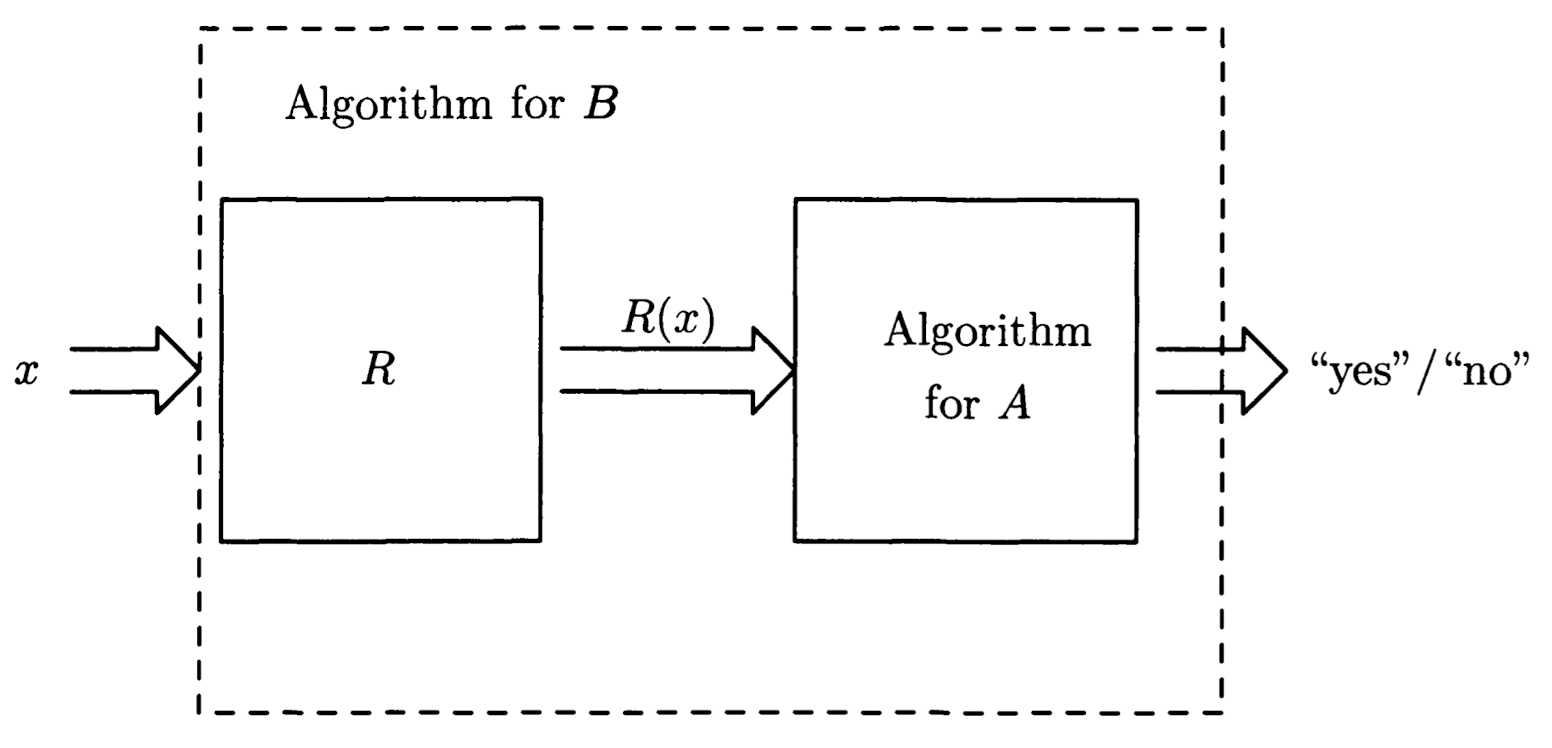
\includegraphics[width=0.9\textwidth]{img/reduction.png}
  \caption{Reduction from $B$ to $A$}
\end{figure}
\\
If the scenario above is possible, it seems reasonable to say that $A$ is at least as hard as $B$. With one proviso: \textit{That $R$ should not be fantastically hard to compute.} If we do not limit the complexity of computing $R$, we could arrive at absurdities such as \textsc{TSP(D)} reduced to \textsc{REACHABILITY}, and thus \textsc{REACHABILITY} being harder than \textsc{TSP(D)}! Indeed, given any instance $x$ of \textsc{TSP(D)} (that is, a distance matrix and a budget), we can apply the following reduction: Examine all tours; if one of them is cheaper than the budget, then $R(x)$ is the two-node graph consisting of a single edge from 1 to 2. Otherwise, it is the two-node graph with no edges. Notice that, indeed, $R(x)$ is a ``yes'' instance of \textsc{REACHABILITY} if and only if $x$ was a ``yes'' instance of \textsc{TSP(D)}. The flaw is, of course, that $R$ is an exponential-time algorithm.
\begin{defbox}[Reduction]
  As we pointed out above, for our concept of reduction to be meaningful, it should involve the weakest computation possible. \emph{We shall adopt $\log n$ space-bounded reduction as our notion of ``efficient reduction.''} That is, we say that language $L_1$ \emph{is reducible to} $L_2$ if there is a function $R$ from strings to strings computable by a deterministic Turing machine in space $\mathcal{O}(\log n)$ such that for all inputs $x$ the following is true: $x \in L_1$ if and only if $R(x) \in L_2$. $R$ is called a \emph{reduction} from $L_1$ to $L_2$. Since our focal problems in complexity involve the comparisons of time classes, it is important to note that reductions are \emph{polynomial-time algorithms}.
  This is because $\textbf{SPACE}(\log n)\subseteq\textbf{TIME}(k^{\log n})\subseteq\textbf{TIME}(n^k)$.
\end{defbox}
\begin{defbox}[Reduction from Hamilton path to SAT]
  Suppose that we are given a graph $G$. We shall construct a Boolean expression $R(G)$ such that $R(G)$ is satisfiable if and only if $G$ has a Hamilton path.
\end{defbox}
  Suppose that $G$ has $n$ nodes, $1,2,\ldots,n$. Then $R(G)$ will have $n^2$ Boolean variables, $x_{ij} : 1 \leq i, j \leq n$. Informally, variable $x_{ij}$ will represent the fact ``node $j$ is the $i$th node in the Hamilton path,'' which of course may be either true or false. $R(G)$ will be in conjunctive normal form, so we shall describe its clauses.

The clauses will spell out all requirements on the $x_{ij}$'s that are sufficient to guarantee that they encode a true Hamilton path. To start, node $j$ must appear in the path; this is captured by the clause $(x_{1j} \vee x_{2j} \vee \ldots \vee x_{nj})$; we have such a clause for each $j$. But node $j$ cannot appear both at $i$th and $k$th; this is expressed by clause $(\neg x_{ij} \vee \neg x_{kj})$, repeated for all values of $j$, and $i \neq k$. Conversely, some node must be $i$th, thus we add the clause $(x_{i1} \vee x_{i2} \vee \ldots \vee x_{in})$ for each $i$; and no two nodes should be $i$th, or $(\neg x_{ij} \vee \neg x_{ik})$ for all $i$, and all $j \neq k$. 

Finally, for each pair $(i,j)$ which is not an edge of $G$, it must not be the case that $j$ comes right after $i$ in the Hamilton path; therefore the following clauses are added for each pair $(i,j)$ not in $G$ and for $k = 1, \ldots, n-1$: $(\neg x_{ki} \vee \neg x_{k+1,j})$. This completes the construction. Expression $R(G)$ is the conjunction of all these clauses.

We claim that $R$ is a reduction from \textsc{Hamilton Path} to \textsc{SAT}. To prove our claim, we have to establish two things: That for any graph $G$, expression $R(G)$ has a satisfying truth assignment if and only if $G$ has a Hamilton path; and that $R$ can be computed in space $\log n$.

Suppose that $R(G)$ has a satisfying truth assignment $T$. Since $T$ satisfies all clauses of $R(G)$, it must be the case that, for each $j$ there exists a unique $i$ such that $T(x_{ij}) = \mathbf{true}$, otherwise the clauses of the form $(x_{1j} \vee x_{2j} \vee \ldots \vee x_{nj})$ and $(\neg x_{ij} \vee \neg x_{kj})$ cannot all be satisfied. Similarly, clauses $(x_{i1} \vee x_{i2} \vee \ldots \vee x_{in})$ and $(\neg x_{ij} \vee \neg x_{ik})$ guarantee that for each $i$ there exists a unique $j$ such that $T(x_{ij}) = \mathbf{true}$. Hence, $T$ really represents a permutation $\pi(1), \ldots, \pi(n)$ of the nodes of $G$, where $\pi(i) = j$ if and only if $T(x_{ij}) = \mathbf{true}$. However, clauses $(\neg x_{k,i} \vee \neg x_{k+1,j})$ where $(i,j)$ is not an edge of $G$ and $k = 1, \ldots, n-1$ guarantee that, for all $k$, $(\pi(k), \pi(k+1))$ is an edge of $G$. This means that $(\pi(1), \pi(2), \ldots, \pi(n))$ is a Hamilton path of $G$. Conversely, suppose that $G$ has a Hamilton path $(\pi(1), \pi(2), \ldots, \pi(n))$, where $\pi$ is a permutation. Then it is clear that the truth assignment $T(x_{ij}) = \mathbf{true}$ if $\pi(i) = j$, and $T(x_{ij}) = \mathbf{false}$ if $\pi(i) \neq j$, satisfies all clauses of $R(G)$.

We still have to show that $R$ can be computed in space $\log n$. Given $G$ as an input, a Turing machine $M$ outputs $R(G)$ as follows: First it writes $n$, the number of nodes of $G$, in binary, and, based on $n$ it generates in its output tape, one by one, the clauses that do not depend on the graph (the first four groups in the description of $R(G)$). To this end, $M$ just needs three counters, $i$, $j$, and $k$, to help construct the indices of the variables in the clauses. For the last group, the one that depends on $G$, $M$ again generates one by one in its work string all clauses of the form $(\neg x_{ki} \vee \neg x_{k+1,j})$ for $k = 1, \ldots, n-1$; after such a clause is generated, $M$ looks at its input to see whether $(i, j)$ is an edge of $G$, and if it is not, then it outputs the clause. This completes our proof that \textsc{Hamilton Path} can be reduced to \textsc{SAT}.

\begin{defbox}[Reduction Composition]
  If $R$ is a reduction from language $L_1$ to $L_2$ and $R'$ is a reduction from language $L_2$ to $L_3$, then the composition $R' \circ R$ is a reduction from $L_1$ to $L_3$.
\end{defbox}
\begin{proof}
  That $x \in L_1$ if and only if $R'(R(x)) \in L_3$ is immediate from the fact that $R$ and $R'$ are reductions. The nontrivial part is to show that $R' \circ R$ can be computed in space $\log n$.

One first idea is to compose the two machines with input and output, $M_R$ and $M_{R'}$, that compute $R$ and $R'$ respectively, so that $R(x)$ is first produced, and from it the final output $R'(R(x))$. Alas, the composite machine $M$ must have $R(x)$ written on a work string; and $R(x)$ may be much longer than $\log |x|$.

The solution to this problem is clever and simple: We do not explicitly store the intermediate result in a string of $M$. Instead, we simulate $M_{R'}$ on input $R(x)$ by remembering at all times the cursor position $i$ of the input string of $M_{R'}$ (which is the output string of $M_R$). $i$ is stored in binary in a new string of $M$. Initially $i = 1$, and we have a separate set of strings on which we are about to begin the simulation of $M_R$ on input $x$.

Since we know that the input cursor in the beginning scans a $\triangleright$, it is easy to simulate the first move of $M_{R'}$. Whenever the cursor of $M_{R'}$'s input string moves to the right, we increment $i$ by one, and continue the computation of machine $M_R$ on input $x$ (on the separate set of strings) long enough for it to produce the next output symbol; this is the symbol currently scanned by the input cursor of $M_{R'}$, and so the simulation can go on. If the cursor stays at the same position, we just remember the input symbol scanned. If, however, the input cursor of $M_{R'}$ moves to the left, there is no obvious way to continue the simulation, since the previous symbol output by $M_R$ has been long forgotten. We must do something more radical: We decrement $i$ by one, and then run $M_R$ on $x$ \textit{from the beginning}, counting on a separate string the symbols output, and stopping when the $i$th symbol is output. Once we know this symbol, the simulation of $M_{R'}$ can be resumed. 

It is clear that this machine indeed computes $R' \circ R$ in space $\log n$ (recall that $|R(x)|$ is at most polynomial in $n = |x|$, and so $i$ has $\mathcal{O}(\log n)$ bits).
\end{proof}
\begin{defbox}[Completeness]
  Let $C$ be a complexity class, and let $L$ be a language in $C$. We say that $L$ is \emph{C-complete} if any language $L'\in C$ can be reduced to $L$.
\end{defbox}
It is not certain that every class $C$ contains a \emph{C-complete} language, but well will see that it's true for the main complexity classes.
\begin{defbox}[Hardness]
  To be precise, given a complexity class $C$, we say that a language $L$ is \emph{C-hard} if every language $L' \in C$ can be reduced to $L$. We say that $L$ is \emph{C-complete} if it is both $C$-hard and in $C$.
\end{defbox}
\begin{defbox}[Closure under reductions]
  We say that a class $C$ is \emph{closed under reductions} if it contains every language $L'$ such that $L\in C$ and $L'$ can be reduced to $L$. That is, if $L\in C$ then $C$ contains every other problem more simple or as hard as $L$.
  $$\textbf{P},\textbf{NP},\textbf{coNP},\textbf{L},\textbf{NL},\textbf{PSPACE}\text{ and } \textbf{EXP} \text{ are all close under reductions.}$$
\end{defbox}
\begin{defbox}[Proposition]
  If two classes $C_1$ and $C_2$ are both closed under reductions, and there is a language $L$ which is complete for both classes, then $C_1=C_2$.
\end{defbox}
\begin{proof}
  Since $L$ is complete for $C_1$, all languages in $C_1$ can be reduced to $L\in C_2$. Since $C_2$ is closed under reductions, it follows that $C_1\subseteq C_2$. The other inclusion follows by symmetry. 
\end{proof}
\begin{defbox}[Colrollary]
  If $C_1 \subseteq C_2$, and $C_1$ is closed under reductions and contains a \emph{$C_2$-complete} language $L$, then $C_1 = C_2$.
\end{defbox}
\begin{proof}
  For the sake of contradiction, suppose that $L'\in C_2\smallsetminus C_1$. For the hypothesis of \emph{$C_2$-completeness}, $L'$ can be reduces to $L\in C_1$. Then for the hypothesis of closure of $C_1$, $L'\in C_1$ which is a contradiction. 
\end{proof}
\subsection{\textcolor{red}{Cook-Levine Theorem}}
\begin{defbox}[\textcolor{red}{Cook-Levine Theorem}]
  \textsc{SAT} is \textbf{NP}-complete.
\end{defbox}
\begin{proof}
  We know that given a satisfiable boolean expression exists a nondeterministic turing machine that is able to find and verify a satisfying assignment in polynomial time. So we have that \textsc{SAT} is in \textbf{NP}. The computation can be represented as a square table with $p(n)$ rows and columns called computation table.  This matrix can be represented as a propositional formula in CNF. We will have a symbol for each cell of the table. Let $\{q_1,\dots,q_r\}$ the states of $M$ and $\{\sigma_1,\dots,\sigma_l\}$ the symbols of the alphabet. For every step $t$ (row) end every cell $s$ (column), that is $(t,s)$ is a coordinate of a cell in the table, we will have:
  \begin{itemize}
    \item $P^i_{s,t}$ (true if cell $(s,t)$ contains symbol $\sigma_i$) $1\le i\le l$
    \item $Q^i_{t}$ (true if the state $q$ at time $t$ is $q_i$) $1\le i\le r$
    \item $S_{s,t}$ (true if the cursor at time $t$ is on cell $s$) $1\le s\le T$ where $T=p(n)$.
  \end{itemize}
  We need to define the following CNF clauses:
  At every step the cursor is on exactly one cell:
  $$\forall t\in\{1,\dots,T\}$$
  \[
\left( \bigvee_{s \in \{1, \dots, T\}} S_{s,t} \right) \land \left( \bigwedge_{1 \leq s < i \leq T} \neg S_{s,t} \lor \neg S_{i,t} \right)
\]
At every step in every cell there is exactly one symbol:
$$\forall s,t\in\{1,\dots,T\}$$
\[
\left( \bigvee_{i \in \{1, \dots, l\}} P^i_{s,t} \right) \land \left( \bigwedge_{1 \leq i < j \leq l} \neg P^i_{s,t} \lor \neg P^j_{s,t} \right)
\]
At every step there is exactly one current state:
$$\forall t\in\{1,\dots,T\}$$
\[
\left( \bigvee_{i \in \{1, \dots, r\}} Q^i_{t} \right) \land \left( \bigwedge_{1 \leq i < j \leq r} \neg Q^i_{t} \lor \neg Q^j_{t} \right)
\]
The initial condition are satisfied if the initial state is $q_1$, the blank $\sigma_2$ ed the initial string $\sigma_{i_1},\dots,\sigma_{i_n}$ (followed by blanks):
$$Q^1_1\land S_{1,1}\land P^{i_1}_{1,1}\land P^{i_2}_{2,1}\land\dots\land P^{i_n}_{n,1}\land P^2_{n+1,1}\land\dots\land P^2_{T,1}$$
 $Q^1_1$ (the initial state is $q_1$), $S_{1,1}$ (the cursor is on cell 1), $P^{i_1}_{1,1}$ (the first symbol of the input string is $\sigma_{i_1}$), $P^{i_2}_{2,1}$ (the second symbol of the input string is $\sigma_{i_2}$), $\dots$, $P^{i_n}_{n,1}$ (the last symbol of the input string is $\sigma_{i_n}$), $P^2_{n+1,1}$ (all other cells are blank), $\dots$, $P^2_{T,1}$ (all other cells are blank). We want that only the symbols under the cursor can change so:
 $$\forall s,t\in\{1,\dots,T\}\; \forall i\in\{1,\dots,I\}$$
 $$\neg S_{s,t}\land P^i_{s,t}\implies P^i_{s,t+1}$$
 written in CNF: 
 $$S_{s,t}\lor \neg P^i_{s,t}\lor P^i_{s,t+1}$$
  The computation accepts the input if the final state $q_k$ = "yes"
  $$Q^k_T$$
  The configurations change as specified by the transition function $\delta$ of $M$. \\
  For all $$(q_i,\sigma_j,q_k,\sigma_m,\la)\not\in\Delta$$
  we have that $\forall t=1,\dots,T-1$ and $\forall s=2,\dots,T$
  $$ Q^i_t\land S_{s,t}\land P^j_{s,t}\implies\neg(Q^k_{t+1}\land P^m_{s,t+1}\land S_{s-1,t+1})$$
  equivalent to the CNF:
  $$\neg Q^i_t\land \neg S_{s,t}\land \neg P^j_{s,t}\land\neg Q^k_{t+1}\land \neg P^m_{s,t+1}\land \neg S_{s-1,t+1}$$
For exercise write the remaining clauses corresponding to the moves $\ra$ e $-$.\\
The reduction $R(x)$ is the \emph{AND} of all the clauses above.
The problem is in \textbf{NP}: Given a satisfiable Boolean expression, a nondeterministic machine can ``guess'' the satisfying truth assignment and verify it in polynomial time. Since we know that \textsc{CIRCUIT SAT} reduces to \textsc{SAT}, we need to show that all languages in $\mathbf{NP}$ can be reduced to \textsc{CIRCUIT SAT}.

Let $L \in \mathbf{NP}$. We shall describe a reduction $R$ which for each string $x$ constructs a circuit $R(x)$ (with inputs that can be either variables or constants) such that $x \in L$ if and only if $R(x)$ is satisfiable. Since $L \in \mathbf{NP}$, there is a nondeterministic Turing machine $M = (K, \Sigma, \Delta, s)$ that decides $L$ in time $n^k$. That is, given a string $x$, there is an accepting computation (sequence of nondeterministic choices) of $M$ on input $x$ if and only if $x \in L$. We assume that $M$ has a single string; furthermore, we can assume that it has at each step \emph{two nondeterministic choices}.
 If for some state-symbol combinations there are $m > 2$ choices in $\Delta$, we modify $M$ by adding $m - 2$ new states so that the same effect is achieved (see Figure below). If for some combination there is only one choice, we consider that the two choices coincide; and finally if for some state-symbol combination there is no choice in $\Delta$, we add to $\Delta$ the choice that changes no state, symbol, or position. So, machine $M$ has exactly two choices for each symbol-state combination. One of these choices is called choice $0$ and the other choice $1$, so that a sequence of nondeterministic choices is simply a bitstring $(c_1, c_2, \ldots, c_{|x|^{k}-1}) \in \{0,1\}^{|x|^{k}-1}$.
 \begin{figure}[ht]
  \centering
  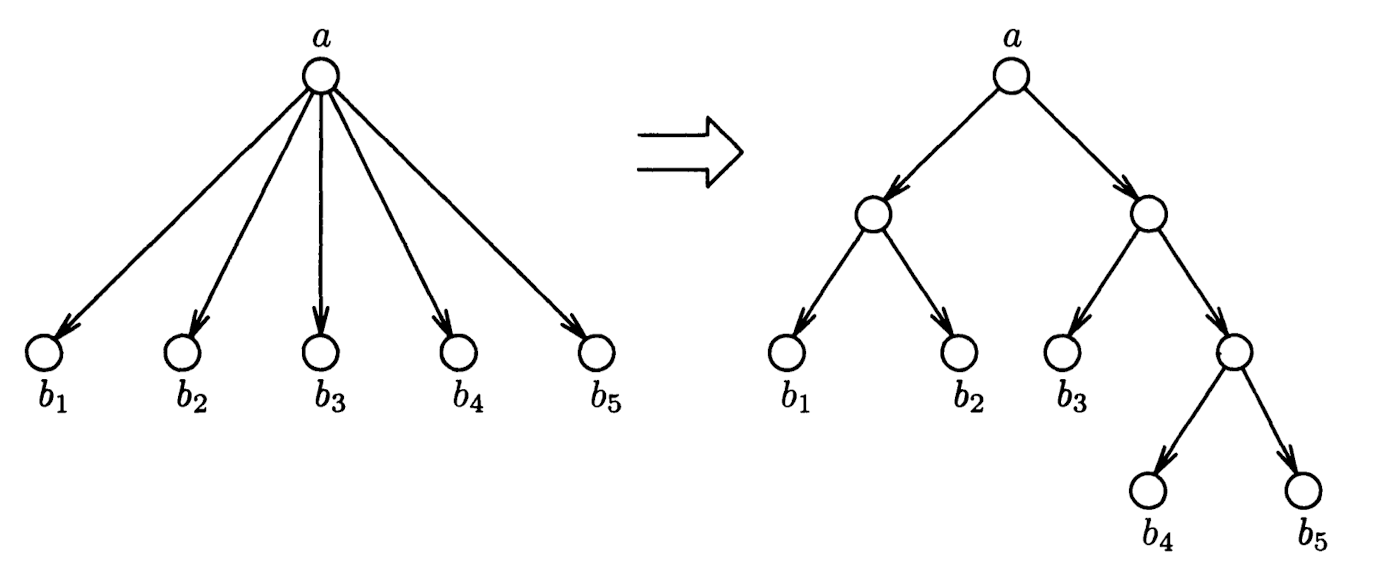
\includegraphics[width=0.7\textwidth]{img/cook.png}
  \caption{Reducing degree of nondeterminism}
\end{figure}
\\
Since the computation of nondeterministic Turing machines proceeds in parallel paths, there is no simple notion of computation table that captures all of the behavior of such a machine on an input. \emph{If, however, we fix a sequence of choices} $\mathbf{c} = (c_0, c_2, \ldots, c_{|x|^k - 1})$, then the computation is effectively deterministic (at the $i$th step we take choice $c_i$), and thus we can define the computation table $T(M, x, \mathbf{c})$ corresponding to the machine, input, and sequence of choices. Again the top row and the extreme columns of the table will be predetermined. All other entries $T_{ij}$ will depend only on the entries $T_{i-1,j-1}$, $T_{i-1,j}$, and $T_{i-1,j+1}$ and the choice $c_{i-1}$ at the previous step (see Figure).
\begin{figure}[ht]
  \centering
  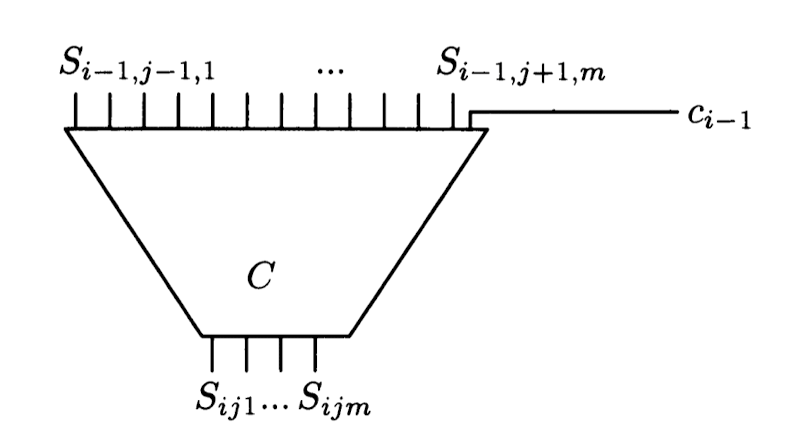
\includegraphics[width=0.5\textwidth]{img/cook2.png}
  \caption{The construction for Cook's theorem}
\end{figure}
\\
That is, this time the fixed circuit $C$ has $3m + 1$ entries instead of $3m$, the extra entry corresponding to the nondeterministic choice.

Thus we can again construct in $\mathcal{O}(\log |x|)$ space a circuit $R(x)$, this time with variable gates $c_0, c_1, \ldots, c_{|x|^k - 1}$ corresponding to the nondeterministic choices of the machine. It follows immediately that $R(x)$ is satisfiable (that is, there is a sequence of choices $c_0, c_1, \ldots, c_{|x|^k - 1}$ such that the computation table is accepting) if and only if $x \in L$.

\end{proof}
\begin{defbox}[3-SAT is NP-complete]
  We also know that \textbf{3-SAT} is \textbf{NP}-complete. We can demonstrate this by reducing \textsc{SAT} to \textsc{3-SAT}. Once we have found a reduction from \textsc{SAT} to \textsc{3-SAT}, we can use the fact that \textsc{SAT} is \textbf{NP}-complete to conclude that \textsc{3-SAT} is also \textbf{NP}-complete. This is because we can reduce every problem in \textbf{NP} to \textsc{SAT}, and then reduce \textsc{SAT} to \textsc{3-SAT}.
\end{defbox}
\begin{defbox}[2-SAT is in P]
  Unlike 3-SAT, we know that \textbf{2-SAT} is in \textbf{P}. This is because we can reduce \textsc{2-SAT} to the search of loops in a graph of linear dimension.
\end{defbox}
\begin{defbox}[Horn clauses]
  A \textbf{Horn clause} is a disjunction of literals with at most one positive literal. A Horn formula is a conjunction of Horn clauses. A Horn formula is satisfiable if and only if it has a satisfying assignment that can be computed in linear time.
\end{defbox}

\newpage
\section{Problems in NP}
Even though there are a lot of different algorithms that can be expressed as nondeterministic Turing machines that alt in polynomial time, the NP problems can be solved with relatively uniform algorithmic strategies. One of the strategies is the \textbf{generate and test}. That is, we generate a possible solutions to the problem and test if it is a solution. This kind of procedure is modeled in abstract with the so called \textbf{polynomially balanced relations}.
\begin{defbox}[Polynomially decidable relations]
Let $R \subseteq \Sigma^* \times \Sigma^*$ be a binary relation on strings. $R$ is called \textbf{polynomially decidable} if there is a deterministic Turing machine deciding the language 
\[
\{x; y : (x, y) \in R\}
\]
in polynomial time. 
\end{defbox}
\begin{defbox}[Polynomially balanced relations]
  We say that $R$ is \textbf{polynomially balanced} if $(x, y) \in R$ implies $|y| \leq |x|^k$ for some $k \geq 1$. That is, the length of the second component is always bounded by a polynomial in the length of the first (the other way is not important).
\end{defbox}
\subsection{\textcolor{red}{Proposition 9.1}}
\begin{defbox}[\textcolor{red}{Proposition 9.1}]
  Let $L \subseteq \Sigma^*$ be a language. $L \in \textbf{NP}$ if and only if there is a polynomially decidable and polynomially balanced relation $R$, such that 
\[
L = \{x : (x, y) \in R \text{ for some } y\}.
\]
\end{defbox}
\begin{proof}
  Suppose that such an $R$ exists. Then $L$ is decided by the following nondeterministic machine $M$: On input $x$, $M$ guesses a $y$ of length at most $|x|^k$ (the polynomial balance bound for $R$), and then uses the polynomial algorithm on $x; y$ to test whether $(x, y) \in R$. If so, it accepts, otherwise it rejects. It is immediate that an accepting computation exists if and only if $x \in L$.

Conversely, suppose that $L \in \textbf{NP}$; that is, there is a nondeterministic Turing machine $N$ that decides $L$ in time $|x|^k$, for some $k$. Define the following relation $R$: $(x, y) \in R$ if and only if $y$ is the encoding of an accepting computation of $N$ on input $x$. It is clear that $R$ is polynomially balanced (since $N$ is polynomially bounded), and polynomially decidable (since it can be checked in linear time whether $y$ indeed encodes an accepting computation of $N$ on $x$). Furthermore, by our assumption that $N$ decides $L$, we have that $L = \{x : (x, y) \in R \text{ for some } y\}$.
\end{proof}
\begin{defbox}[Theorem]
  MAX2SAT is NP-complete.
\end{defbox}
\begin{proof}
  Consider the following ten clauses:
\[
(x)(y)(z)(w)
\]
\[
(\neg x \vee \neg y)(\neg y \vee \neg z)(\neg z \vee \neg x)
\]
\[
(x \vee \neg w)(y \vee \neg w)(z \vee \neg w)
\]

There is no way to satisfy all these clauses (for example, to satisfy all clauses in the first row we must lose all clauses in the second). But how many can we satisfy? Notice first that the clauses are symmetric with respect to $x$, $y$, and $z$ (but not $w$). So, assume that all three of $x$, $y$, $z$ are \textbf{true}. Then the second row is lost, and we can get all the rest by setting $w$ to \textbf{true}. If just two of $x$, $y$, $z$ are \textbf{true}, then we lose a clause from the first row, and one clause from the second row. Then we have a choice: If we set $w$ to \textbf{true}, we get one extra clause from the first row; if we set it to \textbf{false}, we get one from the third. So, we can again satisfy seven clauses, and no more. If only one of $x$, $y$, $z$ is \textbf{true}, then we have one clause from the first row and the whole second row. For the third row, we can satisfy all three clauses by setting $w$ to \textbf{false}, but then we lose $(w)$. The maximum is again seven. However, suppose that all three are \textbf{false}. Then it is easy to see that we can satisfy at most six clauses: The second and third row.

In other words, these ten clauses have the following interesting property: Any truth assignment that satisfies $(x \vee y \vee z)$ can be extended to satisfy seven of them and no more, while the remaining truth assignment can be extended to satisfy only six of them. This suggests an immediate reduction from \textsc{3SAT} to \textsc{MAX2SAT}: Given any instance $\phi$ of \textsc{3SAT}, we construct an instance $R(\phi)$ of \textsc{MAX2SAT} as follows: For each clause $C_i = (\alpha \vee \beta \vee \gamma)$ of $\phi$, we add to $R(\phi)$ the ten clauses above, with $\alpha$, $\beta$, and $\gamma$ replacing $x$, $y$, and $z$; $w$ is replaced by a new variable $w_i$, particular to $C_i$. We call the ten clauses of $R(\phi)$ corresponding to a clause of $\phi$ a group. If $\phi$ has $m$ clauses, then obviously $R(\phi)$ has $10m$ clauses. The goal is set at $K = 7m$.

We claim that the goal can be achieved in $R(\phi)$ if and only if $\phi$ is satisfiable. Suppose that $7m$ clauses can be satisfied in $R(\phi)$. Since we know that in each group we can satisfy at most seven clauses, and there are $m$ groups, seven clauses must be satisfied in each group. However, such an assignment would satisfy all clauses in $\phi$. Conversely, any assignment that satisfies all clauses in $\phi$ can be turned into one that satisfies $7m$ clauses in $R(\phi)$ by defining the truth value of $w_i$ in each group according to how many literals of the corresponding clause of $\phi$ are true.

Finally, it is easy to check that \textsc{MAX2SAT} is in \textbf{NP}, and that the reduction can be carried out in logarithmic space (since these important prerequisites will be very clear in most of the subsequent reductions, we shall often omit mentioning them explicitly).
\end{proof}
\subsection{Graph-theoretic problems}
Many interesting graph-theoretic problems are defined in terms of \textit{undirected graphs}. Technically, an undirected graph is just an ordinary graph which happens to be symmetric and have no self-loops; that is, whenever $(i, j)$ is an edge then $i \neq j$, and $(j, i)$ is also an edge. However, since we shall deal with such graphs extensively, we must develop a better notation for them. 

An undirected graph is a pair $G = (V, E)$, where $V$ is a finite set of nodes and $E$ is a set of unordered pairs of nodes in $V$, called \textit{edges}; an edge between $i$ and $j$ is denoted $[i, j]$. An edge will be depicted as a line (no arrows). \textit{All graphs in this section are undirected.}
Let $G = (V, E)$ be an undirected graph, and let $I \subseteq V$. We say that the set $I$ is \textit{independent} if whenever $i, j \in I$ then there is no edge between $i$ and $j$. All graphs (except for the one with no nodes) have non-empty independent sets; the interesting question is, what is the largest independent set in a graph. The \textsc{INDEPENDENT SET} problem is this: Given an undirected graph $G = (V, E)$, and a goal $K$, is there an independent set $I$ with $|I| = K$?
\begin{defbox}[Theorem]
  INDEPENDENT SET is NP-complete
\end{defbox}
\begin{proof}
  The proof uses a simple gadget, the \textit{triangle}. The point is that if a graph contains a triangle, then any independent set can obviously contain at most one node of the triangle. But there is more to the construction.

Interestingly, to prove that \textsc{INDEPENDENT SET} is \textbf{NP}-complete it is best to \textit{restrict the class of graphs} we consider. Although restricting the domain makes a problem easier, in this case the restriction is such that it retains the complexity of the problem, while making the issues clearer. We consider only graphs \textit{whose nodes can be partitioned in $m$ disjoint triangles} (see Figure).
\begin{figure}[ht]
  \centering
  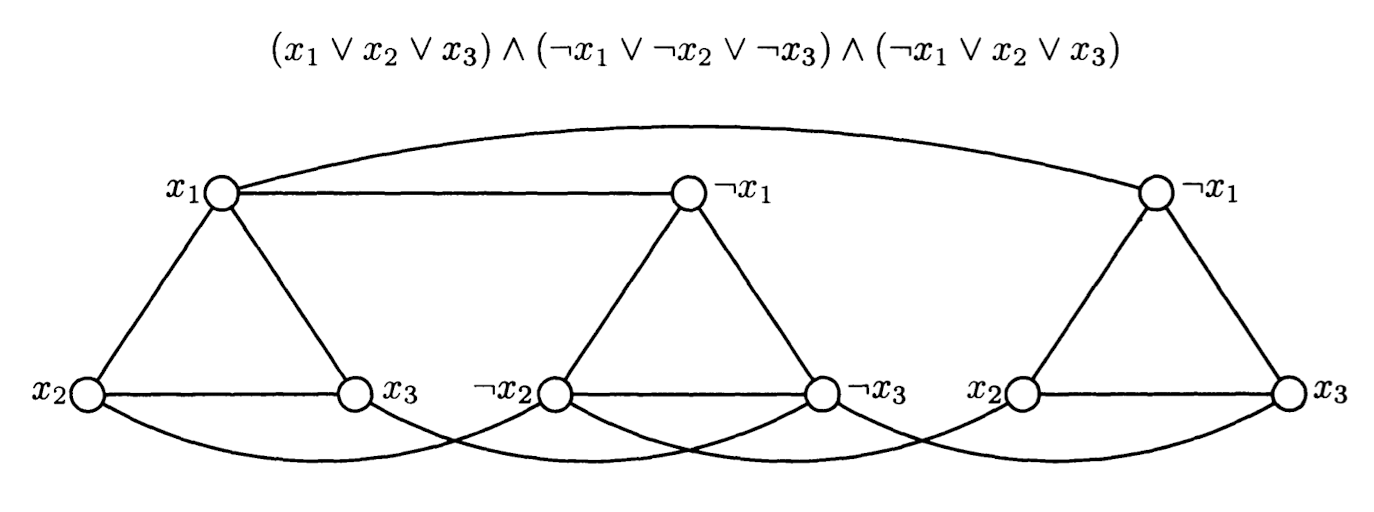
\includegraphics[width=1\textwidth]{img/independent_set.png}
  \caption{Reduction to independent set}
\end{figure}
\\
Then obviously an independent set can contain at most $m$ nodes (one from each triangle); an independent set of size $m$ exists if and only if the other edges of the graph allow us to choose one node from each triangle.

Once we look at such graphs, the combinatorics of the \textsc{INDEPENDENT SET} problem seem easier to understand (and yet no easier to resolve computationally). In fact, a reduction from \textsc{3SAT} is immediate: For each one of the $m$ clauses of the given expression $\phi$ we create a separate triangle in the graph $G$. Each node of the triangle corresponds to a literal in the clause. The structure of $\phi$ is taken into account in this simple manner: We add an edge between two nodes in different triangles \textit{if and only if the nodes correspond to opposite literals} (see Figure 9.2). The construction is completed by taking the goal to be $K = m$.

Formally, we are given an instance $\phi$ of \textsc{3SAT} with $m$ clauses $C_1, \ldots, C_m$, with each clause being $C_i = (\alpha_{i1} \vee \alpha_{i2} \vee \alpha_{i3})$, with the $\alpha_{ij}$'s being either Boolean variables or negations thereof. Our reduction constructs a graph $R(\phi) = (G, K)$, where $K = m$, and $G = (V, E)$ is the following graph: 
\[
V = \{v_{ij} : i = 1, \ldots, m; j = 1, 2, 3\}; 
 \]
 \[ E = \{[v_{ij}, v_{ik}] : i = 1, \ldots, m; j \neq k\} \cup \{[v_{ij}, v_{ek}] : i \neq e, \alpha_{ij} = \neg \alpha_{ek}\}.
\]
(There is a node for every appearance of a literal in a clause; the first set of edges defines the $m$ triangles, and the second group joins opposing literals.)

We claim that there is an independent set of $K$ nodes in $G$ if and only if $\phi$ is satisfiable. Suppose that such a set $I$ exists. Since $K = m$, $I$ must contain a node from each triangle. Since the nodes are labeled with literals, and $I$ contains no two nodes corresponding to opposite literals, $I$ is a truth assignment that satisfies $\phi$: The \textit{true} literals are just those which are labels of nodes of $I$ (variables left unassigned by this rule can take any value). We know that this gives a truth assignment because any two contradictory literals are connected by an edge in $G$, and so they cannot both be in $I$. And since $I$ has a node from every triangle, the truth assignment satisfies all clauses. Conversely, if a satisfying truth assignment exists, then we identify a \textit{true} literal in each clause, and pick the node in the triangle of this clause labeled by this literal: This way we collect $m = K$ independent nodes. 
\end{proof}
Even if the graph is planar, the \textsc{INDEPENDENT SET} problem remains \textbf{NP}-complete (see Problem 9.5.9). However, it is polynomially solvable when the graph is bipartite (see Problem 9.5.25). The reason for this is that, in bipartite graphs, \textsc{INDEPENDENT SET} is closely related to \textsc{MATCHING}, which in turn is a special case of \textsc{MAX FLOW}.

This brings about an interesting point: Problems in graph theory can be guises of one another in confusing ways; sometimes this suggests trivial reductions from a problem to another. In the \textsc{CLIQUE} problem we are given a graph $G$ and a goal $K$, and we ask whether there is a set of $K$ nodes that form a \textit{clique} by having all possible edges between them. Also, \textsc{NODE COVER} asks whether there is a set $C$ with $B$ or fewer nodes (where $B$ is a given ``budget;'' this is a minimization problem) such that each edge of $G$ has at least one of its endpoints in $C$.
\begin{defbox}[Corollary]
  CLIQUE and NODE COVER are NP-complete
\end{defbox}
\begin{proof}
  It is easy to see that \textsc{CLIQUE} is a clumsy disguise of \textsc{INDEPENDENT SET}: If we take the \textit{complement} of the graph, that is, a graph that has precisely those edges that are missing from this one, cliques become independent sets and vice-versa. Also, $I$ is an independent set of graph $G = (V, E)$ if and only if $V - I$ is a node cover of the same graph (and, moreover, \textsc{NODE COVER} is, conveniently, a minimization problem)
\end{proof}
\begin{defbox}[Theorem]
  The \textsc{HAMILTON PATH} problem is NP-complete.
  Recall that the \textsc{HAMILTON PATH} problem is the problem of deciding whether a given graph $G$ has a path that visits every node exactly once and ends at the starting node.   
\end{defbox}
\begin{proof}
  The fact that \textsc{HAMILTON PATH} is in \textbf{NP} is immediate: Given a path, we can check in linear time whether it visits every node exactly once. To prove the hardness of the problem, we reduce \textsc{3SAT} to it.
\end{proof}
\begin{defbox}[Theorem]
  \textsc{TSP(D)} is NP-complete
\end{defbox}
\begin{proof}
  An instance of \textsc{TSP(D)} is a complete graph. Every node of the instance of \textsc{Hamilton path} is a city. If two cities are connected by an edge, then the distance between them is 1. If two cities are not connected by an edge, then the distance between them is 2. The goal is to find a Hamiltonian cycle of length $n$ in the graph. Thus, we can reduce \textsc{TSP(D)} to \textsc{HAMILTON PATH}.
\end{proof}
\begin{defbox}[Theorem]
  \textsc{3-COLORING} is NP-complete
\end{defbox}
\begin{proof}
  Recall that the \textsc{K-COLORING} problem is the problem of deciding whether a given graph can be colored with k colors such that no two adjacent nodes have the same color. The \textsc{2-COLORING} problem is in P. Now let's dimostrate that \textsc{3-COLORING} is NP-complete. To prove that \textsc{3-COLORING} is in NP, is easy. We can generate nondeterministically a color for every node and check in polynomial time if the graph is 3-colorable.
  The total cost in $O(n^3)$. To prove that \textsc{3-COLORING} is NP-complete, we can reduce \textsc{3SAT} to \textsc{3-COLORING}. We will use 2 gadget. The first one codifies the truth assignments.
  \\
  \begin{figure}[ht]
  \centering
  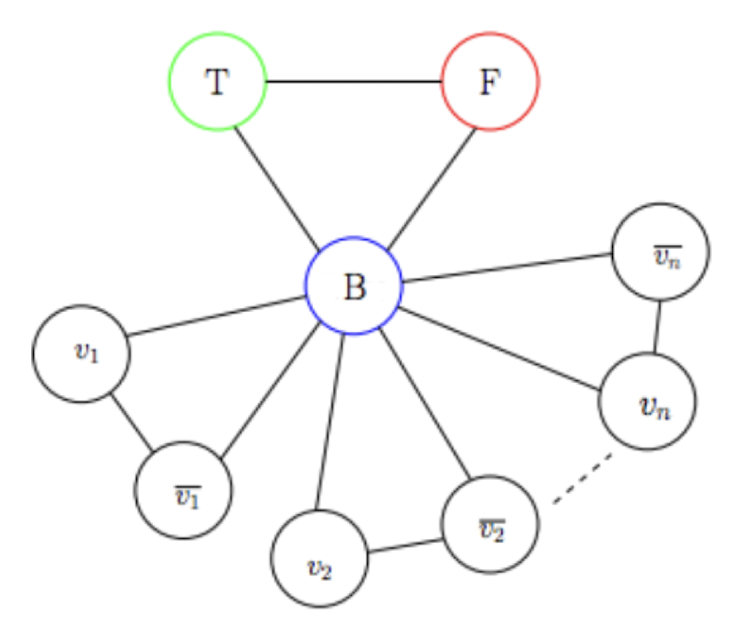
\includegraphics[width=0.5\textwidth]{img/3-coloring-1g.png}
  \caption{1st gadget}
  \end{figure}
  \\
   Every proposition $v_i$ is colored as $T$ or $F$. Every negative literal $\overline{v_i}=\neg v_i$ is colored the opposite way. The second gadget codifies the OR. If $p,q$ are both colored with $F$ then $p\vee q$ is $F$ as well otherwise it can always be colored with $T$.
   \\
   \begin{figure}[ht]
    \centering
    \begin{subfigure}[b]{0.3\textwidth}
        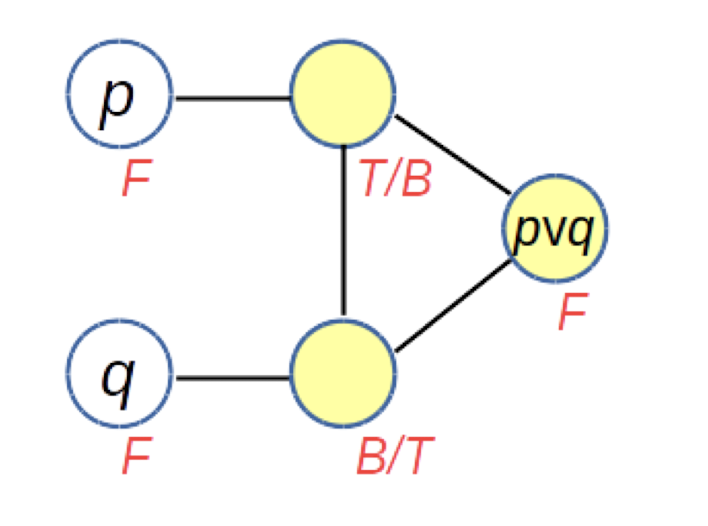
\includegraphics[width=\textwidth]{img/3-coloring-2g.png}
        \caption{case 1}
        \label{fig:img1}
    \end{subfigure}
    \hfill
    \begin{subfigure}[b]{0.3\textwidth}
        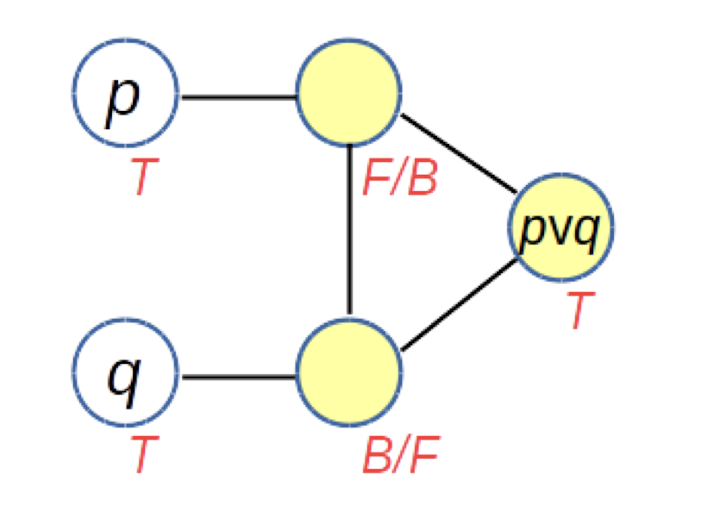
\includegraphics[width=\textwidth]{img/3-coloring-2g2.png}
        \caption{case 2}
        \label{fig:img2}
    \end{subfigure}
    \hfill
    \begin{subfigure}[b]{0.3\textwidth}
        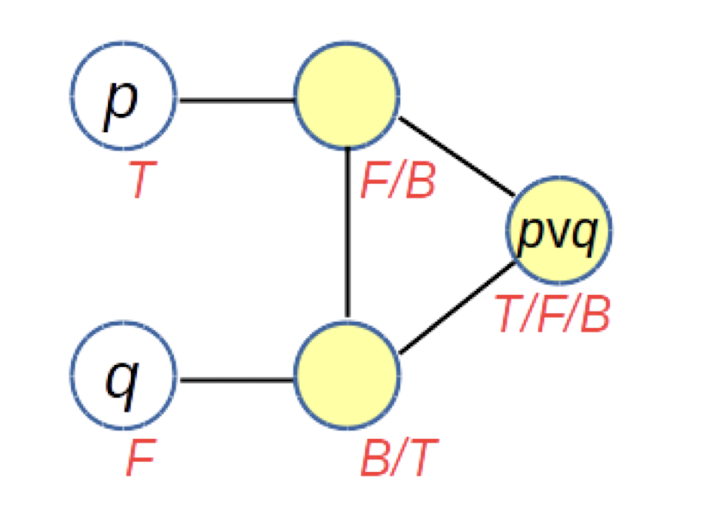
\includegraphics[width=\textwidth]{img/3-coloring-2g3.png}
        \caption{case 3}
        \label{fig:img3}
    \end{subfigure}
    \caption{2nd gadget}
    \label{fig:images}
\end{figure}
\\
The or are connected in cascade to represent the 3 clauses. If $a,b,c$ are colored with F the $a\vee b\vee c$ is colored with F as well otherwise it can be colored with T. 
\begin{figure}[ht]
  \centering
  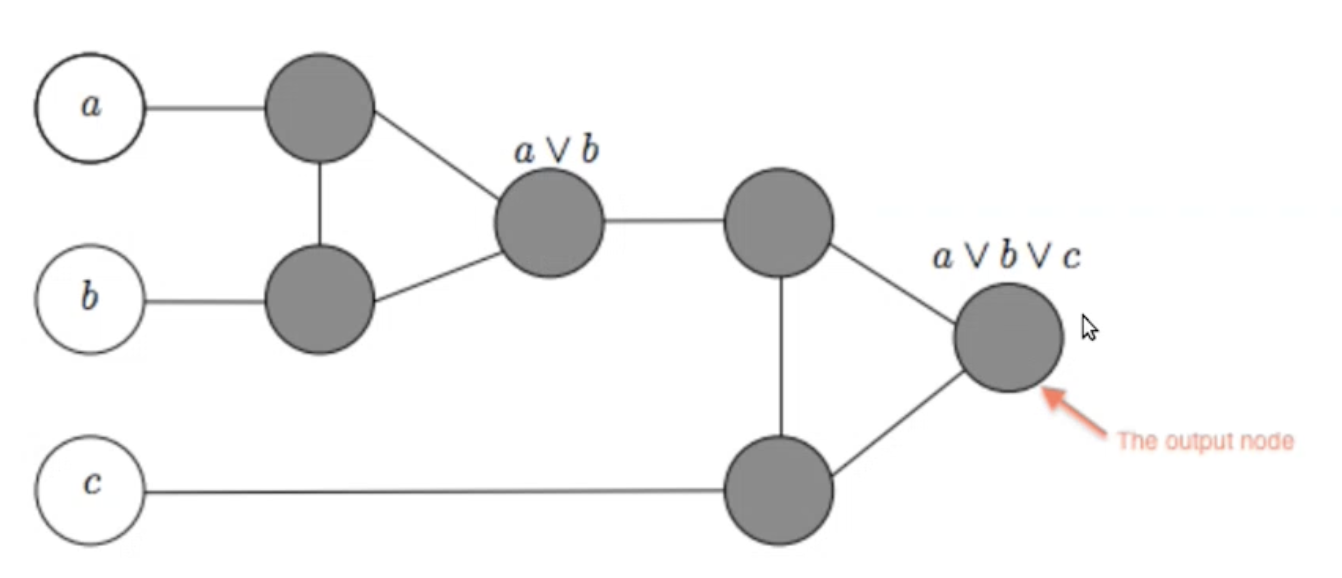
\includegraphics[width=0.5\textwidth]{img/3-coloring-3g.png}
  \caption{OR cascade}
\end{figure}
\\
To ensure that the clauses are satisfied we connect the clauses output like this:
\\
\begin{figure}[ht]
  \centering
  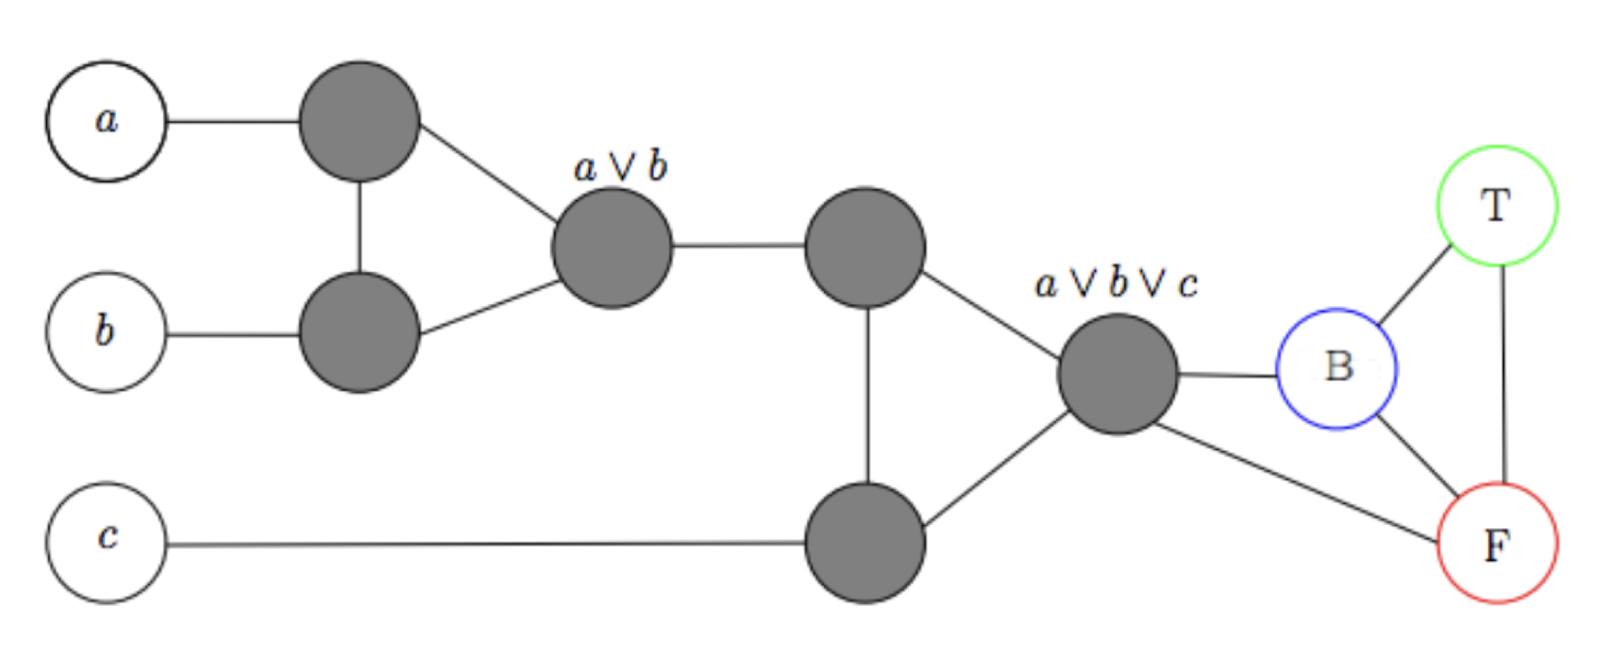
\includegraphics[width=0.5\textwidth]{img/3-coloring-4g.png}
  \caption{Final graph}
\end{figure}
\\
This way we can ensure that the clauses are satisfied because at least one of the literals must be colored with T otherwise the final node would be colored with F.
\end{proof}
Complete example:\\
\begin{figure}[ht]
  \centering
  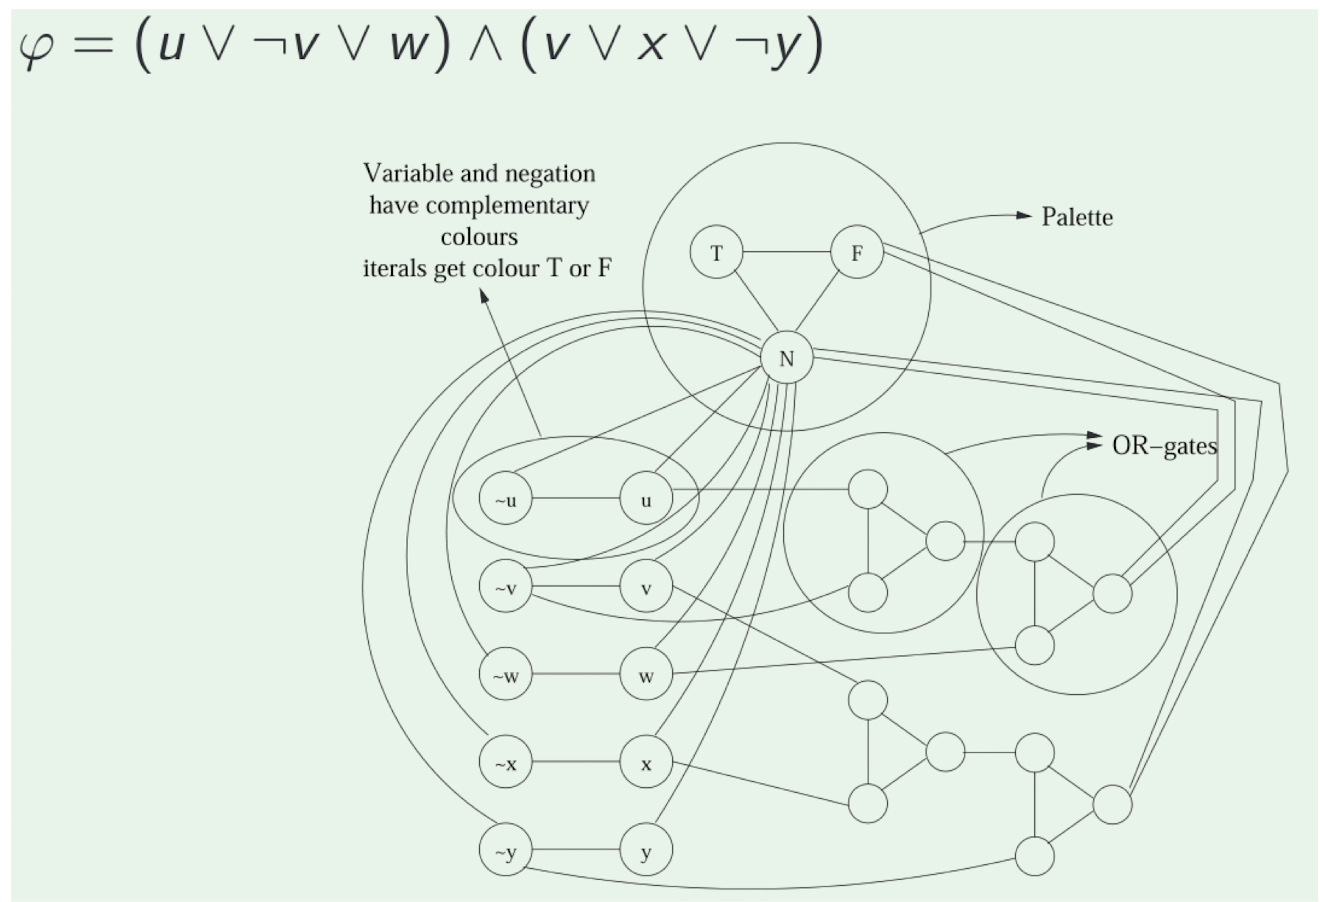
\includegraphics[width=0.9\textwidth]{img/3-coloring-example.png}
  \caption{complete example}
\end{figure}
\subsection{Problems on sets}
Suppose that we are given three sets $B$, $G$, and $H$ (boys, girls, and homes), each containing $n$ elements, and a ternary relation $T \subseteq B \times G \times H$. We are asked to find a set of $n$ triples in $T$, no two of which have a component in common—that is, each boy is matched to a different girl, and each couple has a home of its own. We call this problem \textsc{TRIPARTITE MATCHING}.
\begin{defbox}[Theorem]
  \textsc{TRIPARTITE MATCHING} is NP-complete.
\end{defbox}
\begin{proof}
  omitted (lezione 11-1 28:40)
\end{proof}
There are some other interesting problems involving sets, that we define next. In \textsc{SET COVERING} we are given a family $F = \{S_1, \ldots, S_n\}$ of subsets of a finite set $U$, and a budget $B$. We are asking for a set of $B$ sets in $F$ whose union is $U$. In \textsc{SET PACKING} we are also given a family of subsets of a set $U$, and a goal $K$; this time we are asked if there are $K$ pairwise disjoint sets in the family. In a problem called \textsc{EXACT COVER BY 3-SETS} we are given a family $F = \{S_1, \ldots, S_n\}$ of subsets of a set $U$, such that $|U| = 3m$ for some integer $m$, and $|S_i| = 3$ for all $i$. We are asked if there are $m$ sets in $F$ that are disjoint and have $U$ as their union.

We can show all these problems \textbf{NP}-complete by pointing out that they are all generalizations of \textsc{TRIPARTITE MATCHING}. This is quite immediate in the case of \textsc{EXACT COVER BY 3-SETS}; \textsc{TRIPARTITE MATCHING} is the special case in which $U$ can be partitioned into three equal sets $B$, $G$, and $H$, such that each set in $F$ contains one element from each. Then, it is easy to see that \textsc{EXACT COVER BY 3-SETS} is the special case of \textsc{SET COVERING} in which the universe has $3m$ elements, all sets in $F$ have three elements, and the budget is $m$. Similarly for \textsc{SET PACKING}.
\begin{defbox}[Corollary]
\textsc{EXACT COVER BY 3-SETS}, \textsc{SET COVERING}, and \textsc{SET PACKING} are NP-complete.
\end{defbox}
\subsection{Integer programming}
\textsc{INTEGER PROGRAMMING} asks whether a given system of linear inequalities, in $n$ variables and with integer coefficients, has an integer solution. We have already seen more than a dozen reasons why this problem is \textbf{NP}-complete: All problems we have seen so far can be easily expressed in terms of linear inequalities over the integers. For example, \textsc{SET COVERING} can be expressed by the inequalities 
\[
Ax \geq 1; \quad \sum_{i=1}^n x_i \leq B; \quad 0 \leq x_i \leq 1,
\]
where each $x_i$ is a $0 - 1$ variable which is one if and only if $S_i$ is in the cover, $A$ is the matrix whose rows are the bit vectors of the sets, $1$ is the column vector with all entries $1$, and $B$ is the budget of the instance. Hence \textsc{INTEGER PROGRAMMING} is \textbf{NP}-complete (the hard part is showing that it is in \textbf{NP}; see the notes at the end of the chapter). In contrast, \textsc{LINEAR PROGRAMMING}, the same problem without the requirement that the solutions be integers, is in \textbf{P} (see the discussion in 9.5.34).

We shall next look at a very special case of \textsc{INTEGER PROGRAMMING}. The \textsc{KNAPSACK} problem looks at the following situation. We must select some among a set of $n$ items. Item $i$ has value $v_i$, and weight $w_i$, both positive integers. There is a limit $W$ to the total weight of the items we can pick. We wish to pick certain items (without repetitions) to maximize the total value, subject to the constraint that the total weight is at most $W$. That is, we are looking for a subset $S \subseteq \{1, \ldots, n\}$ such that 
\[
\sum_{i \in S} w_i \leq W, \quad \text{and} \quad \sum_{i \in S} v_i \text{ is as large as possible.}
\]
In the recognition version, called \textsc{KNAPSACK}, we are also given a goal $K$, and we wish to find a subset $S \subseteq \{1, \ldots, n\}$ such that 
\[
\sum_{i \in S} w_i \leq W \quad \text{and} \quad \sum_{i \in S} v_i \geq K.
\]
\begin{defbox}[Theorem]
  \textsc{KNAPSACK} is NP-complete.
\end{defbox}
\begin{proof}
  This is another case in which restricting the problem facilitates the \textbf{NP}-completeness proof. We are going to look at the special case of \textsc{KNAPSACK} in which $v_i = w_i$ for all $i$, and $K = W$. That is, we are given a set of $n$ integers $w_1, \ldots, w_n$, and another integer $K$, and we wish to find out if a subset of the given integers adds up to exactly $K$. This simple numerical problem turns out to be \textbf{NP}-complete.

We shall reduce \textsc{EXACT COVER BY 3-SETS} to it. We are given an instance $\{S_1, S_2, \ldots, S_n\}$ of \textsc{EXACT COVER BY 3-SETS}, where we are asking whether there are disjoint sets among the given ones that cover the set $U = \{1, 2, \ldots, 3m\}$. Think of the given sets as bit vectors in $\{0, 1\}^{3m}$. Such vectors can also be thought as binary integers, and set union now resembles integer addition (see Figure).
\begin{figure}[ht]
  \centering
  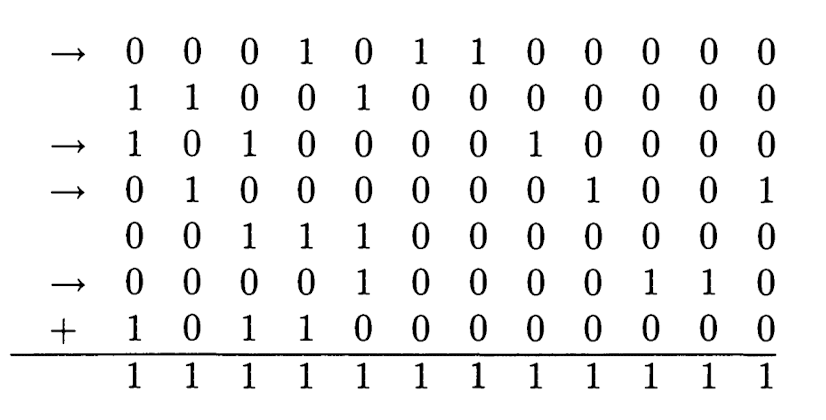
\includegraphics[width=0.5\textwidth]{img/knapsack.png}
  \caption{Reduction to knapsack}
\end{figure}
\\
 Our goal is to find a subset of these integers that add up to exactly $K$.

Let $K = 2^n - 1$ (the all-ones vector, corresponding to the universe). The reduction seems complete!

But there is a ``bug'' in this reduction: Binary integer addition is different from set union in that it has carry. For example, $3 + 5 + 7 = 15$ in bit-vector form is $0011 + 0101 + 0111 = 1111$; but the corresponding sets $\{3, 4\}, \{2, 4\},$ and $\{2, 3, 4\}$ are not disjoint, neither is their union $\{1, 2, 3, 4\}$. There is a simple and clever way around this problem: Think of these vectors as integers not in base 2, but in base $n + 1$. That is, set $S_i$ becomes integer $w_i = \sum_{j \in S_i} (n + 1)^{3m-j}$. 

Since now there can be no carry in any addition of up to $n$ of these numbers, it is straightforward to argue that there is a set of these integers that adds up to $K = \sum_{j=0}^{3m-1} (n + 1)^j$ if and only if there is an exact cover among $\{S_1, S_2, \ldots, S_n\}$. 
\end{proof}
\subsection{Pseudopolynomial Algorithms and strong NP-completeness}
\begin{defbox}[Proposition]
  Any instance of \textsc{KNAPSACK} can be solved in $\mathcal{O}(nW)$ time, where $n$ is the number of items and $W$ is the weight limit.
\end{defbox}
\begin{proof}
  Define $V(w, i)$ to be the largest value attainable by selecting some among the $i$ first items so that their total weight is exactly $w$. It is easy to see that the $nW$ entries of the $V(w, i)$ table can be computed in order of increasing $i$, and with a constant number of operations per entry, as follows:
\[
V(w, i+1) = \max\{V(w, i), v_{i+1} + V(w - w_{i+1}, i)\}.
\]
To start, $V(w, 0) = 0$ for all $w$. Finally, the given instance of \textsc{KNAPSACK} is a ``yes'' instance if and only if the table contains an entry greater than or equal to the goal $K$. 
\end{proof}
This algorithm is called \textbf{pseudopolynomial} because it runs in polynomial time with respect to the value of the input, but not with respect to the size(representation) of the input. 
$W=O(2^{|W|})$ so the problem \textsc{P=NP} is not solved. If we use small integers we can solve the problem in polynomial time. But if we use big integers we can not solve the problem in polynomial time.
Naturally, the above proposition does not establish that $\mathbf{P} = \mathbf{NP}$ (so, keep on reading this book!). This is not a polynomial algorithm because its time bound $nW$ is not a polynomial function of the input: The length of the input is something like $n \log W$. We have seen this pattern before in our first attempt at an algorithm for \textsc{MAX FLOW}, when the time required was again polynomial in the integers appearing in the input (instead of their logarithms, which is always the correct measure). Such ``pseudopolynomial'' algorithms are a source not only of confusion, but of genuinely positive results.

In relation to pseudopolynomial algorithms, it is interesting to make the following important distinction between \textsc{KNAPSACK} and the other problems that we showed \textbf{NP}-complete in this chapter---\textsc{SAT}, \textsc{MAX CUT}, \textsc{TSP (D)}, \textsc{CLIQUE}, \textsc{TRIPARTITE MATCHING}, \textsc{HAMILTON PATH}, and many others. All these latter problems were shown \textbf{NP}-complete via reductions that constructed only \textit{polynomially small integers}. For problems such as \textsc{CLIQUE} and \textsc{SAT}, in which integers are only used as node names and variable indices, this is immediate. But even for \textsc{TSP (D)}, in which one would expect numbers to play an important role as intercity distances, we only needed distances no larger than two to establish \textbf{NP}-completeness. In contrast, in our \textbf{NP}-completeness proof for \textsc{KNAPSACK} we had to create \textit{exponentially large integers} in our reduction.
\begin{defbox}[Strong NP-completeness]
If a problem remains \textbf{NP}-complete even if any instance of length $n$ is restricted to contain integers of size at most $p(n)$, a polynomial, then we say that the problem is \textit{strongly NP-complete}. All \textbf{NP}-complete problems that we have seen so far in this chapter, with the single exception of \textsc{KNAPSACK}, are strongly \textbf{NP}-complete. It is no coincidence then that, of all these problems, only \textsc{KNAPSACK} can be solved by a pseudopolynomial algorithm: It should be clear that strongly \textbf{NP}-complete problems have no pseudopolynomial algorithms, unless of course $\mathbf{P} = \mathbf{NP}$.
\end{defbox}
\subsection{Exercises}
\subsubsection{exercise 1}
Given a graph:
\begin{figure}[ht]
  \centering
  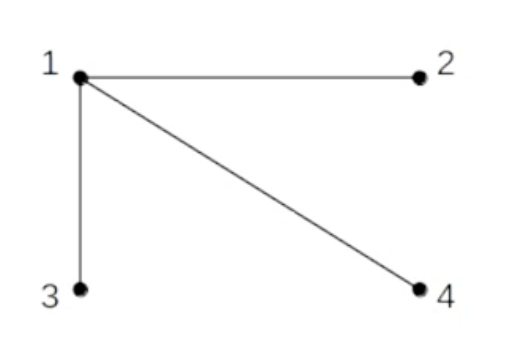
\includegraphics[width=0.5\textwidth]{img/es1.png}
\end{figure}
\\
- The independent sets (that is, the sets of nodes that are not connected) are: $$\{\}, \{1\}, \{2\}, \{3\}, \{4\}, \{3,4\}, \{3,2\}, \{4,2\}, \{3,4,2\}$$
- The clique sets (that is, the sets of nodes that are strongly connected) are: 
$$ \{\}, \{1\}, \{2\}, \{3\}, \{4\}, \{1,3\}, \{1,2\}, \{1,4\} $$
- The node cover sets (that is, the sets of nodes that are connected to all the other nodes) are:
$\{1\}$\\
- Provide a succinct certificate for the instance of node cover made up of this graph and $K=2$ (that is a minimization problem where we want to find the set of at max 2 nodes that is connected to all the other nodes):
$\{1\}$
\subsubsection{exercise 2}
Premise: The fragment of Schönfinkel-Bernays is a formula of first order logic where there are no function symbols, no equality, and in prenex normal form (that is, all the quantifiers are at the beginning of the formula). Schönfinkel-Bernays SAT problem has been shown to be NEXP-complete.
Tell if there exists a reduction form the following problems:
\begin{itemize}
  \item \textsc{SAT} to \textsc{TSP(D)}\\
  YES, because they are both NP-complete problems.
  \item \textsc{TSP(D)} to \textsc{SAT}\\
  YES, because they are both NP-complete problems.
  \item \textsc{HAMILTON PATH} to \textsc{SET COVER}\\
  YES, because they are both NP-complete problems.
  \item \textsc{SET COVER} to \textsc{HAMILTON PATH}\\
  YES, because they are both NP-complete problems.
  \item \textsc{CLIQUE} to \textsc{2-SAT}\\
  Would be true if \textsc{P=NP} but we don't know that.
  \item \textsc{2-SAT} to \textsc{CLIQUE}\\
  YES, because \textsc{2-SAT} is in P and \textsc{CLIQUE} is NP-complete.
  \item \textsc{2-SAT} to \textsc{Schönfinkel-Bernays SAT}\\
  YES, because \textsc{2-SAT} is in P and \textsc{Schönfinkel-Bernays SAT} is NEXP-complete.
  \item \textsc{Schönfinkel-Bernays SAT} to \textsc{2-SAT}\\
  NO, because \textsc{Schönfinkel-Bernays SAT} is NEXP-complete and \textsc{2-SAT} is in P. We know that $P\subset EXP$ so it is impossible to have a reduction from NEXP-complete to P.
  \item \textsc{MAX FLOW} to \textsc{3-COLORING}\\
  YES, because \textsc{MAX FLOW} is in P and \textsc{3-COLORING} is NP-complete.
  \item \textsc{3-COLORING} to \textsc{MAX FLOW}\\
  Would be true if \textsc{P=NP} but we don't know that.
\end{itemize}
\subsubsection{exercise 3}
Specify a format for a succinct certificate for the \textsc{3-COLORING} problem (that is, a string no too long with respect to the input that represents a solution to the problem). A valid format could be a string with the couples $(i,j)$ where $i$ is the node and $j$ is the color. The node index could be in positional representation so it would be a string of length $O(\log n)$ and the color could be a single character. So the final string would be of length $O(n \log n)$ which is polynomial with respect to the input.\\
Show a certificate for the following graph:
\begin{figure}[ht]
  \centering
  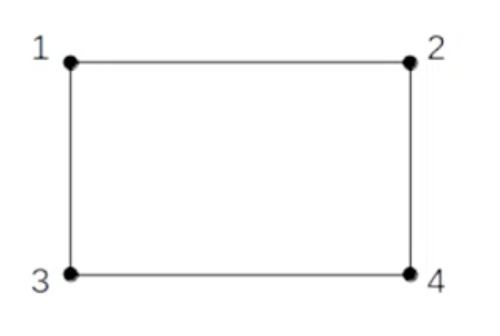
\includegraphics[width=0.5\textwidth]{img/es3.png}
\end{figure}
\\
A possible certificate could be:
$001,r;010,b;011,b;100,g$

\newpage
\section{coNP}
If $NP$ is the class of problems that have succinct certificates (recall Theorem 9.1), then $coNP$ must contain those problems that have \textit{succinct disqualifications}. That is, a ``no'' instance of a problem in $coNP$ possesses a short proof of its being a ``no'' instance; and only ``no'' instances have such proofs.

\textbf{Example:} \textit{VALIDITY of Boolean expressions} is a typical problem in $coNP$. We are given a Boolean expression $\phi$, and we are asked whether it is valid, satisfiable by all truth assignments. If $\phi$ is not a valid formula, then it can be disqualified very succinctly: By exhibiting a truth assignment that does not satisfy it. No valid formula has such a disqualification.

For another example, \textit{HAMILTON PATH COMPLEMENT} is the set of all graphs that have no Hamilton path. Since it is the complement of the \textit{HAMILTON PATH problem}\footnote{Recall that we say two languages are complements of each other if they are disjoint and their union is, not necessarily the set of all strings, but some other, trivial to recognize set; in this case, the set of all strings that are legitimate encodings of graphs.}, it is in $coNP$. Here the disqualification is, naturally enough, a Hamilton path: All ``no'' instances of \textit{HAMILTON PATH COMPLEMENT}, and only these, have one. We should also mention here \textit{SAT COMPLEMENT}; but in some sense we already have: \textit{VALIDITY} is just \textit{SAT COMPLEMENT} with the expression negated.

Needless to say, all problems that are in $P$ are ex officio in $coNP$, since $P \subseteq NP$ is a deterministic complexity class, and therefore closed under complement.

\textit{VALIDITY} and \textit{HAMILTON PATH COMPLEMENT} are examples of $coNP$-complete problems. We claim that any language $L$ in $coNP$ is reducible to \textit{VALIDITY}. In proof, if $L \in coNP$ then $\overline{L} \in NP$, and thus there is a reduction $R$ from $\overline{L}$ to \textit{SAT}. For any string $x$ we have $x \in \overline{L}$ if and only if $R(x)$ is satisfiable. The reduction from $L$ to \textit{VALIDITY} is this: $R'(x) = \neg R(x)$. The proof for \textit{HAMILTON PATH COMPLEMENT} is very similar. More generally, we have:

\begin{defbox}[Definition of complement of language/problem]
 Given $L\subseteq I$, the complement of $L$ is defined as $\overline{L} = I \smallsetminus L$. 
 Given a complexity class $C$, 
 $$\overline{L}\in co\textsc{C} \iff L\in C$$
 So \coNP is the class of languages $\overline{L}$ whose complement $L\in\textsc{NP}$.
\end{defbox}
\subsection{\textcolor{red}{Propositions A-D}}
\begin{defbox}[\textcolor{red}{Proposition A}]
  If $R$ is a reduction from $L$ to $L'$ then $R$ is also a reduction from $\overline{L}$ to $\overline{L'}$
\end{defbox}
\begin{proof}
  For hypothesis, $$x\in L\iff R(x)\in L'$$
  Then, 
  $$x\in \overline{L} \iff x\notin L \iff R(x)\notin L' \iff R(x)\in \overline{L'}$$
  same for the other direction.
\end{proof}
\begin{defbox}[\textcolor{red}{Proposition B}]
If $L$ is \textsc{NP}-complete, then its complement $\overline{L} = \Sigma^* - L$ is $coNP$-complete.
\end{defbox}
\begin{proof}
  Since $L$ is \textsc{NP}-complete, we know that $\overline{L}$ is in $coNP$. Now let's prove that $\overline{L}$ is $coNP$-complete. Let $\overline{L'}\in \coC (L'\in \textsc{C})$. For hp there exist a reduction $R$ from $L'$ to $L$. Por the  proposition A, we have that $R$ is also a reduction from $\overline{L'}$ to $\overline{L}$. Since this is true for every $\overline{L'}\in\coC$, we can conclude that $\overline{L}$ is $coNP$-complete.
  The other way is proven by symmetry.
\end{proof}

\begin{defbox}[\textcolor{red}{Proposition C}]
  If $C$ is closed under reduction, then co\textsc{C} is closed under reduction.
\end{defbox}
\begin{proof}
  Let $C$ be close under reduction. Let $L\in\coC$ and suppose there exist a reduction $R$ from $L'$ to $L$. We need to prove that $L'\in\coC$.
  For proposition A, we have that $R$ is also a reduction from $\overline{L}$ to $\overline{L'}$. $\overline{L}\in C$ and $C$ is closed under reduction, so $\overline{L'}\in C$. So $L'\in \coC$.
\end{proof}

\begin{defbox}[\textcolor{red}{Proposition D}]
  If $C$ is closed under reduction and a \C-complete problem is in co\textsc{C} then \C=\coC
\end{defbox}
\begin{proof}
  Let $L\in\coC$ be a \C-complete problem. Let first prove that $\C\subseteq\coC$. For every $L'\in\C$, there exists a reduction $R$ from $L'$ to $L$ (because $L$ is \C-complete). Since $L\in\coC$ and co\textsc{C} is closed under reduction for proposition C, then $L'\in\coC$. So $\C\subseteq\coC$. Since $L$ is \C-complete, we have that $\overline{L}\in\coC$ is \coC-complete for proposition B. Since $L'\in\coC$, there exist a reduction $R: L'\to\overline{L}$. We know that $L\in\C$ because $L$ is \C-complete and $L\in\coC$ for hypothesis. So $L\in\C\cap\coC$. For this we can also say that $\overline{L}\in\C\cap\coC$. Since there is a reduction $R: L'\to\overline{L}$ then $L'\in\C$. So $\coC\subseteq\C$. We have that $\C\subseteq\coC$ and $\coC\subseteq\C$ so $\C=\coC$. 
\end{proof}
Whether $NP = coNP$ is another fundamental question that is as important as it is unresolved (you will encounter many more of these). Of course, if after all it turns out that $P = NP$, then $NP = coNP$ will also hold, since $P$ is closed under complement. Conceivably it could be that $P \neq NP$, and still $NP = coNP$. But it is strongly believed that $NP$ and $coNP$ are different. All efforts to find systematic ways for deriving short proofs of \textit{VALIDITY}, for example, have failed. Similarly, we know of no characterizations of non-Hamiltonian graphs that would allow us to demonstrate the absence of a Hamilton path succinctly.

The problems in $coNP$ that are $coNP$-complete are the least likely to be in $P$. What is more, \textit{they are also the least likely to be in $NP$}.
\begin{defbox}[Proposition]
  $$P\subseteq \textsc{NP}\cap\coNP$$
\end{defbox}
\begin{proof}
  Let $L\in P$. Then $\overline{L}\in P$ because $P$ is closed under complement. Since $L$ is also in $NP$ because $P\subseteq NP$, we have that $\overline{L}\in NP$. So for definition of $coNP$, we have that $L\in\coNP$.
\end{proof}
  So, problems in $NP$ have succinct certificates, whereas problems in $coNP$ have succinct disqualifications. $NP \cap coNP$ is the class of problems that have both! That is, problems in $NP \cap coNP$ have the following property: Each instance either has a succinct certificate (in which case it is a ``yes'' instance) or it has a succinct disqualification (in which case it is a ``no'' instance). No instance has both. The nature of certificates and disqualifications will be very different, and different algorithms will be used to validate them. But exactly one of the two always exists. Obviously, any problem in $P$ is also in $NP \cap coNP$, but there are examples of problems in $NP \cap coNP$ that are not known to be in $P$.
\subsection{Exercises}
\subsubsection{exercise 1}
Tell if there is a reduction between the following problems:
\begin{itemize}
  \item \textsc{SAT} to \textsc{VALIDITY}\\
  \textsc{SAT}$\in NP$ and \textsc{VALIDITY}$\in coNP$ so would be true if \textsc{NP=coNP} but we don't know that.
  \item \textsc{VALIDITY} to \textsc{SAT}\\
  Same as above.
  \item \textsc{PRIMES} to \textsc{2-SAT}\\
  Yes, because \textsc{PRIMES} is in P and \textsc{2-SAT} is P-complete.
  \item \textsc{2-SAT} to \textsc{PRIMES}\\
  Would be true if \textsc{PRIMES} were P-complete but we don't know that.
  \item \textsc{PRIMES} to $\overline{\textsc{TSP(D)}}$\\
  Yes, because \textsc{PRIMES} is in P and $\overline{\textsc{TSP(D)}}$ is co\textsc{NP}-complete.
  \item $\overline{\textsc{TSP(D)}}$ to \textsc{PRIMES}\\
  Would be true if \textsc{PRIMES} were P-complete and P=co\textsc{NP}=\textsc{NP} but we don't know that.
  \item \textsc{PRIMES} to \textsc{CLIQUE}\\
  Yes, because \textsc{CLIQUE} is NP-complete and \textsc{PRIMES} is in P.
  \item \textsc{CLIQUE} to \textsc{PRIMES}\\
  Would be true if \textsc{PRIMES} were P-complete and P=\textsc{NP} but we don't know that.
\end{itemize}
\subsubsection{exercise 2}
Assume that $\NP\not=\coNP$. Tell if there exist a reduction between the following problems:
\begin{itemize}
  \item \textsc{SAT} to \textsc{VALIDITY}\\
  No, because \textsc{SAT} is NP-complete and \textsc{VALIDITY} is co\textsc{NP}-complete. So if there was a reduction from \textsc{SAT} to \textsc{VALIDITY} then we would have that \textsc{NP}=\textsc{coNP}.
  \item \textsc{VALIDITY} to \textsc{SAT}\\
  Same as above.
  \item \textsc{CLIQUE} to \textsc{PRIMES}\\
  No, because \textsc{CLIQUE} is NP-complete and \textsc{PRIMES} is in P. So if there was a reduction from \textsc{CLIQUE} to \textsc{PRIMES} then we would have that \textsc{NP}=\textsc{P}=\textsc{coNP}.
  \item \textsc{PRIMES} to \textsc{CLIQUE}\\
  Yes, because \textsc{PRIMES} is in P and \textsc{CLIQUE} is NP-complete.
  \item \textsc{NODE COVER} to \textsc{2-SAT}\\
  No, because \textsc{NODE COVER} is NP-complete and \textsc{2-SAT} is in P. So if there was a reduction from \textsc{NODE COVER} to \textsc{2-SAT} then we would have that \textsc{NP}=\textsc{P}=\textsc{coNP}.
  \item \textsc{2-SAT} to \textsc{NODE COVER}\\
  Yes, because \textsc{2-SAT} is in P and \textsc{NODE COVER} is NP-complete.
  \item \textsc{PRIMES} to \textsc{KNAPSACK}\\
  Yes, because \textsc{PRIMES} is in P and \textsc{KNAPSACK} is NP-complete.
  \item \textsc{KNAPSACK} to \textsc{PRIMES}\\
  No, because \textsc{KNAPSACK} is NP-complete and \textsc{PRIMES} is in P. So if there was a reduction from \textsc{KNAPSACK} to \textsc{PRIMES} then we would have that \textsc{NP}=\textsc{P}=\textsc{coNP}.
  \item \textsc{MAX-FLOW} to \textsc{3-COLORING}\\
  Yes, because \textsc{MAX-FLOW} is in P and \textsc{3-COLORING} is NP-complete.
  \item \textsc{3-COLORING} to \textsc{MAX-FLOW}\\
  No, because \textsc{3-COLORING} is NP-complete and \textsc{MAX-FLOW} is in P. So if there was a reduction from \textsc{3-COLORING} to \textsc{MAX-FLOW} then we would have that \textsc{NP}=\textsc{P}=\textsc{coNP}.
\end{itemize}
\subsubsection{exercise 3}
Let $L_1$ be \textsc{PSPACE}-complete and $L_2$ be \textsc{NPSPACE}-complete. Tell if there exist a reduction between $L_1$ and $L_2$.


Yes, because \textsc{PSPACE} = \textsc{NPSPACE}. So it is true for both directions.

\section{Optimization problems}
Optimization problems have not been classified in a satisfactory way within the theory of $P$ and $NP$; it is these problems that motivate the immediate extensions of this theory beyond $NP$.

Let us take the traveling salesman problem as our working example. In the problem \textit{TSP} we are given the distance matrix of a set of cities; we want to find the shortest tour of the cities. We have studied the complexity of the \textit{TSP} within the framework of $P$ and $NP$ only indirectly: We defined the decision version \textit{TSP (D)}, and proved it $NP$-complete. For the purpose of understanding better the complexity of the traveling salesman problem, we now introduce two more variants.

\textbf{EXACT TSP:} Given a distance matrix and an integer $B$, is the length of the shortest tour \textit{equal to} $B$? Also,  

\textbf{TSP COST:} Given a distance matrix, compute the length of the shortest tour.

The four variants can be ordered in ``increasing complexity'' as follows:
\[
\text{TSP (D); \quad EXACT TSP; \quad TSP COST; \quad TSP.}
\]

Each problem in this progression can be reduced to the next. For the last three problems this is trivial; for the first two one has to notice that the reduction in the corollary to the theorem proving that \textit{TSP (D)} is $NP$-complete can be used to reduce \textit{HAMILTON PATH} to \textit{EXACT TSP} (the graph has a Hamilton path if and only if the optimum tour has length \textit{exactly} $n + 1$). And since \textit{HAMILTON PATH} is $NP$-complete and \textit{TSP (D)} is in $NP$, we must conclude that there is a reduction from \textit{TSP (D)} to \textit{EXACT TSP}.

Actually, we know that these four problems are \textit{polynomially equivalent} (since the first and the last one are). That is, there is a polynomial-time algorithm for one if and only if there is for all four. Admittedly, from the point of view of the practical motivation for complexity theory (namely, to identify problems that are likely to require exponential time) this coarse characterization should be good enough. However, reductions and completeness provide far more refined and interesting categorizations of problems. In this sense, of these four variants of the \textit{TSP} we know the precise complexity only of the $NP$-complete problem \textit{TSP (D)}. In this section we shall show that the other three versions of the \textit{TSP} are complete for some very natural extensions of $NP$. Is the \textit{EXACT TSP} in $NP$? Given a distance matrix and the alleged optimum cost $B$, how can we certify succinctly that the optimum cost is indeed $B$? The reader is invited to ponder about this question; no obvious solution comes to mind. It would be equally impressive if we could certify that the optimum cost \textit{is not} $B$; in other words, \textit{EXACT TSP} does not even appear to be in $coNP$. In fact, the results in this section will suggest that if \textit{EXACT TSP} is in $NP \cup coNP$, this would have truly remarkable consequences; the world of complexity would have to be vastly different than it is currently believed.

However, \textit{EXACT TSP} is closely related to $NP$ and $coNP$ in at least one important way: Considered as a language, \textit{it is the intersection of a language in $NP$} (the \textit{TSP} language) \textit{and one in $coNP$} (the language \textit{TSP COMPLEMENT}, asking whether the optimum cost is \textit{at least} $B$). In other words, an input is a ``yes'' instance of \textit{EXACT TSP} if and only if it is a ``yes'' instance of \textit{TSP}, and a ``yes'' instance of \textit{TSP COMPLEMENT}. This calls for a definition:
\begin{defbox}[Definition of DP Class]
  A language $L$ is in the class \textit{DP} if and only if there are two languages $L_1 \in NP$ and $L_2 \in coNP$ such that $L = L_1 \cap L_2$.
\end{defbox}
We should warn the reader immediately against a quite common misconception: \textit{DP is not} $NP \cap coNP$\footnote{We mean, these two classes are not known or believed to be equal. In the absence of a proof that $P \neq NP$ one should not be too emphatic about such distinctions.}. There is a world of difference between these two classes. For one thing, \textit{DP} is not likely to be contained even in $NP \cup coNP$, let alone the much more restrictive $NP \cap coNP$. The intersection in the definition of $NP \cap coNP$ is in the domain of \textit{classes of languages}, not languages as with \textit{DP}.

For another important difference between $NP \cap coNP$ and \textit{DP}, the latter is a perfectly syntactic class, and therefore has \textit{complete problems}. Consider for example the following problem:

\textbf{SAT-UNSAT:} Given two Boolean expressions $\phi, \phi'$, both in conjunctive normal form with three literals per clause. Is it true that $\phi$ is satisfiable and $\phi'$ is not?
\begin{defbox}[Theorem]
    \textit{SAT-UNSAT} is \textit{DP}-complete.
\end{defbox}
\begin{proof}
    To show that it is in \textit{DP} we have to exhibit two languages $L_1 \in NP$ and $L_2 \in coNP$ such that the set of all ``yes'' instances of \textit{SAT-UNSAT} is $L_1 \cap L_2$. This is easy: 
\[
L_1 = \{(\phi, \phi') : \phi \text{ is satisfiable}\} \quad \text{and} \quad L_2 = \{(\phi, \phi') : \phi' \text{ is unsatisfiable}\}.
\]

To show completeness, let $L$ be any language in \textit{DP}. We have to show that $L$ reduces to \textit{SAT-UNSAT}. All we know about $L$ is that there are two languages $L_1 \in NP$ and $L_2 \in coNP$ such that $L = L_1 \cap L_2$. Since \textit{SAT} is $NP$-complete, we know that there is a reduction $R_1$ from $L_1$ to \textit{SAT}, and a reduction $R_2$ from the complement of $L_2$ to \textit{SAT}. The reduction from $L$ to \textit{SAT-UNSAT} is this, for any input $x$:
\[
R(x) = (R_1(x), R_2(x)).
\]

We have that $R(x)$ is a ``yes'' instance of \textit{SAT-UNSAT} if and only if $R_1(x)$ is satisfiable and $R_2(x)$ is not, which is true if and only if $x \in L_1$ and $x \in L_2$, or equivalently $x \in L$.
\end{proof}

\textbf{OTHER DP-COMPLETE PROBLEMS:}
\begin{itemize}[label=$\blacksquare$]
    \item \textbf{EXACT TSP}
    \begin{itemize}[label=$\bullet$]
        \item We already shown the is in DP, the hardness cna be obtained by reduction from \textit{SAT-UNSAT}.
    \end{itemize}
    
    \item \textbf{CRITICAL SAT}
    \begin{itemize}[label=$\bullet$]
        \item Given $\phi$ in CNF, tell if is unsatisfiable but removing any clause would make it satisfiable.
    \end{itemize}
    
    \item \textbf{CRITICAL HAMILTON PATH}
    \begin{itemize}[label=$\bullet$]
        \item The given graph doesn't have hamiltonian paths, but adding any edge would make it have one.
    \end{itemize}
    
    \item \textbf{CRITICAL 3-COLORING}
    \begin{itemize}[label=$\bullet$]
        \item The given graph is not 3-colorable, but removing any edge would make it 3-colorable.
    \end{itemize}
\end{itemize}
    
\textbf{UNIQUE SAT}: Given $\phi$ in CNF, tell if it has only one satisfying assignment. We don't know if it is \textit{DP}-complete we only know that it is in \textit{DP} and we don't know if it is in a smaller class. 

\newpage
\section{Oracle Machines}
\begin{defbox}[TM with oracle]
  Is a multitape TM with a special tape that can be used to ask questions to an oracle. It also have 3 special states: $q_?,q_{YES},q_{NO}$. $M^?$ is like a template, given a problem $L$, we have $M^L$ where the 3 special states are use to question the oracle whether the input is in $L$ or not. The state $q_?$ is used to ask the oracle, $q_{YES}$ and $q_{NO}$ are the possible answers. The oracle is not part of the TM, it is a black box that can be used to ask questions regarding $L$. In addition to the standard TM transitions we have the following transitions:
\[
  (q_?, w_1, u_1, \dots, w_k, u_k) \xrightarrow{M} (q_{ans}, w_1, u_1, \dots, w_k, u_k)
\]
where if the query tape is the i-th tape and $w_iu_i=\tr x$ then:
\begin{itemize}[label=$\bullet$]
  \item $q_{ans}=q_{YES}$ if $x \in L$
  \item $q_{ans}=q_{NO}$ if $x \notin L$
\end{itemize}
The resources used by the oracle are hidden, the answer is given in a single step and the space used is the space needed to write the query. 
\end{defbox}
\begin{defbox}[Class with Oracle]
  If $C$ is the class of problems that cab be solved in a certain amount of time/space with a turing machine of some kind (deterministic or not) then $C^L$ is the class of problems that can be solved in the same amount of time/space with the same kind of turing machine with oracle $L$.
\end{defbox}
\newpage
\textbf{EXAMPLE}: Turing machine with oracle for \textsc{SAT-UNSAT}.\\
The machine starts by copying the first part of the input $x;y$, that is $x$, on the second tape. Then it asks the oracle whether $x$ is satisfiable or not. The oracle will answer with $q_{YES}$ or $q_{NO}$. If the answer is $q_{NO}$ it rejects,but if the answers is $q_{YES}$ then the machine will clear the second tape and write $y$ on it. Then it asks the oracle whether $y$ is satisfiable or not. If the answer is $q_{NO}$ then the machine will accept, otherwise it will reject. 
\begin{table}[ht]
\begin{center}
\renewcommand{\arraystretch}{1.2}
\begin{tabular}{|c|c|c|c|c|c|c|c|l|}
\hline
\textbf{State} & \textbf{R 1} & \textbf{R 2} & \textbf{NS} & \textbf{W 1} & \textbf{M 1} & \textbf{W 2} & \textbf{M 2} & \textbf{Note} \\
\hline
$s$ & $\triangleright$ & $\triangleright$ & $s$ & $\triangleright$ & $\rightarrow$ & $\triangleright$ & $\rightarrow$ & \\
$s$ & $x$ & $\blank$ & $s$ & $x$ & $\rightarrow$ & $x$ & $\rightarrow$ & $x \neq ;,\ x \neq \sqcup$ \\
$s$ & $;$ & $\blank$ & $q_?$ & $;$ & $-$ & $\blank$ & $-$ & \\
$q_{YES}$ & $;$ & $\blank$ & $r$ & $;$ & $-$ & $\blank$ & $\la$ & \\
$q_{NO}$ & $;$ & $\blank$ & \texttt{"no"} & $;$ & $-$ & $\blank$ & $-$ & \\
$r$ & $;$ & $x$ & $r$ & $;$ & $-$ & $\blank$ & $\leftarrow$ & $x \neq \triangleright$ \\  
$r$ & $;$ & $\triangleright$ & $a$ & $;$ & $\ra$ & $\triangleright$ & $\rightarrow$ & \\
$a$ & $x$ & $\blank$ & $a$ & $x$ & $\rightarrow$ & $x$ & $\ra$ & $x \neq \sqcup$ \\
$a$ & $\sqcup$ & $\sqcup$ & $q_?$ & $\sqcup$ & $-$ & $\sqcup$ & $-$ & \\
$q_{YES}$ & $\sqcup$ & $\sqcup$ & \texttt{"no"} & $\sqcup$ & $-$ & $\sqcup$ & $-$ & \\
$q_{NO}$ & $\sqcup$ & $\sqcup$ & \texttt{"yes"} & $\sqcup$ & $-$ & $\sqcup$ & $-$ &  \\
\hline
\end{tabular}
\\
\end{center}
\textsc{In all other cases reject}
\caption{Transizioni della Macchina di Turing con stati speciali e oracolo}
\end{table}
\newpage
\begin{defbox}[Proposition]
  For every language $L$ \textsc{NP}-complete, $P^L=P^{SAT}$.
\end{defbox}
\begin{proof}
  The proof is by reduction. We can reduce any problem in \textsc{NP} to \textsc{SAT} because \textsc{SAT} is \textsc{NP}-complete. The same thing holds for \textsc{L} since it is \textsc{NP}-complete.
\end{proof}
Since every oracle can be reduced to the others complete problems of the same class, we can use the complexity class it belongs to.\\
\textbf{EXAMPLE}: $P^{NP}, NP^{NP}, EXP^{NP}$ instead of $P^{SAT}, NP^{TSP(D)}, EXP^{CLIQUE}$,\dots
\begin{defbox}[Proposition]
  $C^D=C^{coD}$
\end{defbox}
\begin{proof}
  To prove this we can simply observe that if the switch the $q_{YES}$ and $q_{NO}$ states we can obtain a reduction from one to the other.\\
\end{proof}
We can se $P^{NP}$ as a generalization of $DP$. Obviously  $DP \subseteq P^{NP}$.
Some oracles are useless, for example $P^{P} = P$ and $NP^{P} = NP$ because every call to the oracle can be expanded in line without changing the complexity of the problem. We 't know if $NP^{NP} = NP$. We will analyze this problem in the next section.





\section{Polynomial Hierarchy}
\begin{figure}[h]
    \centering
    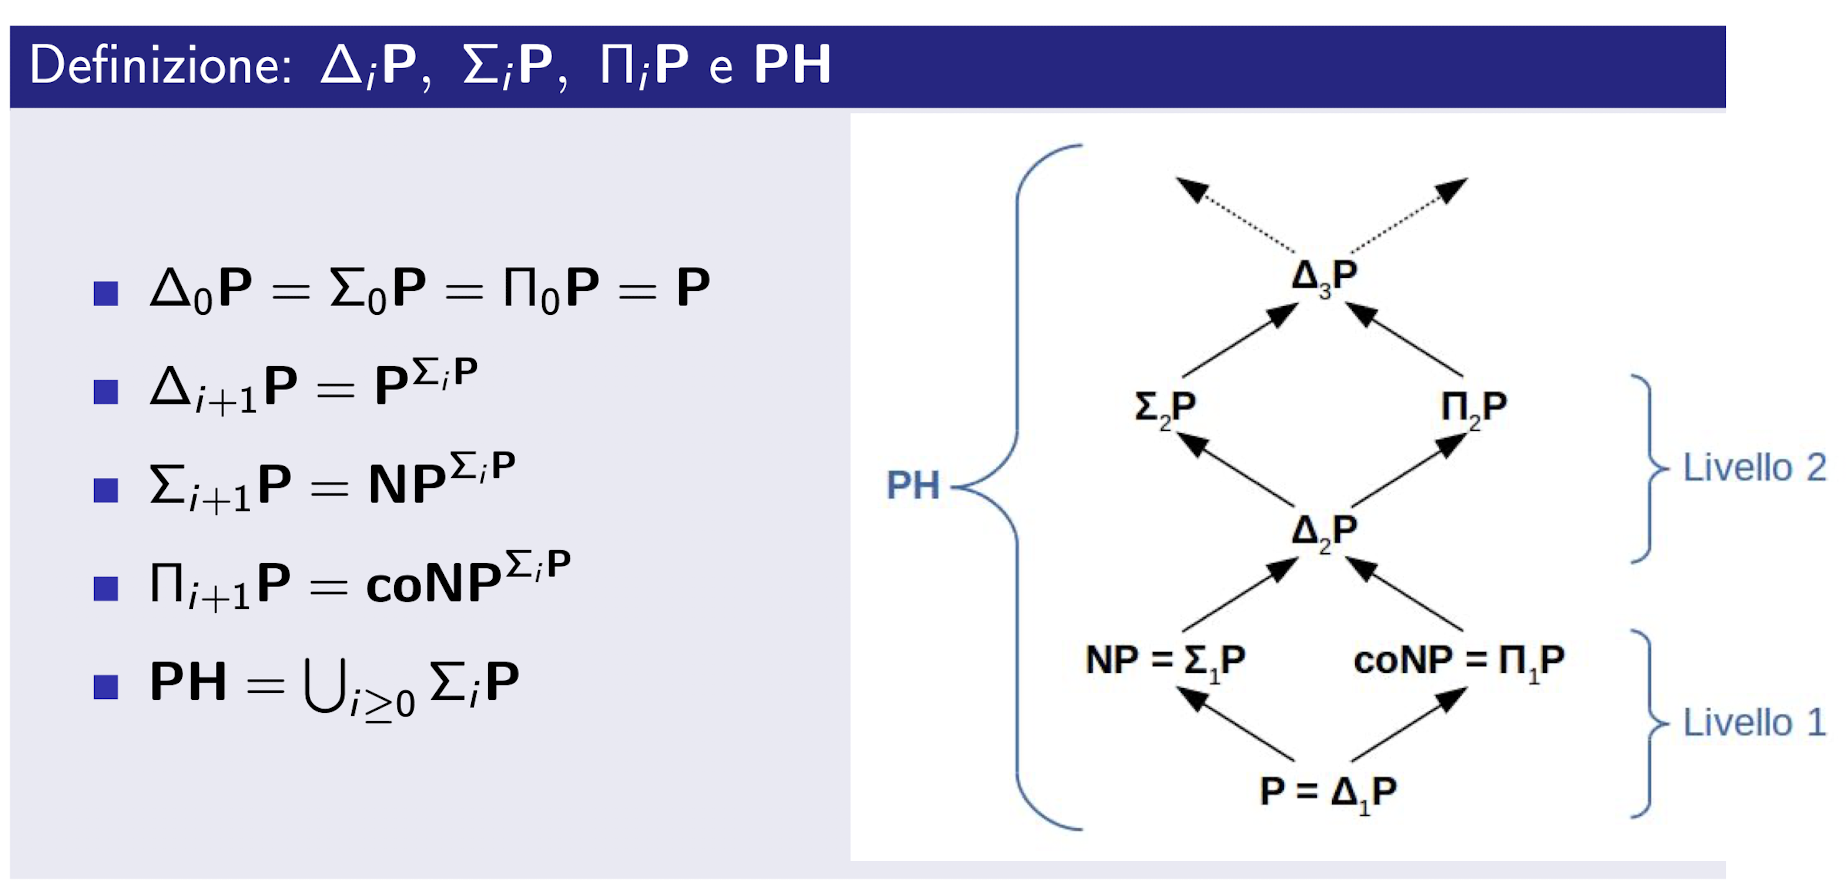
\includegraphics[width=1\textwidth]{img/ph.png}
    \caption{Polynomial Hierarchy}
\end{figure}
Since $\Sigma_0\mathbf{P} = \mathbf{P}$ does not help polynomial-time oracle machines, the first level of this hierarchy makes up our familiar important complexity classes: 
\[
\Delta_1\mathbf{P} = \mathbf{P}, \quad \Sigma_1\mathbf{P} = \mathbf{NP}, \quad \Pi_1\mathbf{P} = \mathbf{coNP}.
\]
The second level starts with the class $\Delta_2\mathbf{P} = \mathbf{P}^{\mathbf{NP}}$ studied in the previous section, and continues with $\Sigma_2\mathbf{P} = \mathbf{NP}^{\mathbf{NP}}$, and its complement $\Pi_2\mathbf{P} = \mathbf{coNP}^{\mathbf{NP}}$. As with the first level, there is every reason to believe that all three classes are distinct. The same holds for the third level, and so on. Naturally, the three classes at each level are related by the same inclusions that we know about $\mathbf{P}$, $\mathbf{NP}$, and $\mathbf{coNP}$. Also, each class at each level includes all classes at previous levels.
\begin{defbox}[Theorem 17.8]
Let $L$ be a language, and $i \geq 1$. $L \in \Sigma_i\mathbf{P}$ if and only if there is a polynomially balanced relation $R$ such that the language $\{x; y : (x, y) \in R\}$ is in $\Pi_{i-1}\mathbf{P}$ and
\[
L = \{ x : \text{there is a } y \text{ such that } (x, y) \in R \}
\]
\end{defbox}
\begin{proof}
    omitted
\end{proof}
\begin{defbox}[Corollary 1]
Let $L$ be a language, and $i \geq 1$. $L \in \Pi_i\mathbf{P}$ if and only if there is a polynomially balanced binary $R$ such that the language $\{x; y : (x, y) \in R\}$ is in $\Sigma_{i-1}\mathbf{P}$ and
\[
L = \left\{ x : \text{ for all } y \text{ with } |y| \leq |x|^k,\, (x, y) \in R \right\}.
\]
\end{defbox}
\begin{proof}
Just recall that $\Pi_i\mathbf{P}$ is precisely $\mathbf{co}\Sigma_i\mathbf{P}$.
\end{proof}
Notice that in the description of $L$ in Corollary 1 we must explicitly state for the universally quantified string $y$ the bound $|y| \leq |x|^k$. Since $R$ is known to be polynomially balanced, this constraint is, in this context, superfluous, and will be omitted. Also, we shall use quantifiers such as $\forall x$ and $\exists y$ in the descriptions of languages such as the one displayed in Corollary 2 below. This will help bring out the elegant mathematical structure of these descriptions, as well as their affinity with logic.

\medskip

In order to get rid of the recursion in the previous Theorem, let us call a relation $R \subseteq (\Sigma^*)^{i+1}$ polynomially balanced if, whenever $(x, y_1, \ldots, y_i) \in R$, we have that $|y_1|, \ldots, |y_i| \leq |x|^k$ for some $k$.
\begin{defbox}[Corollary 2]
Let $L$ be a language, and $i \geq 1$. $L \in \Sigma_i\mathbf{P}$ if and only if there is a polynomially balanced, polynomial-time decidable $(i+1)$-ary relation $R$ such that
\[
L = \left\{ x : \exists y_1 \forall y_2 \exists y_3 \cdots Q y_i \text{ such that } (x, y_1, \ldots, y_i) \in R \right\}
\]
where the $i$th quantifier $Q$ is ``for all'' if $i$ is even, and ``there is'' if $i$ is odd.
\end{defbox}
\begin{proof}
    Repeatedly replace languages in $\Pi_j\mathbf{P}$ or $\Sigma_j\mathbf{P}$ by their certificate forms as in Theorem and its Corollary 1.
\end{proof}
Using these characterizations we can prove the basic fact concerning the polynomial hierarchy: As it is built by patiently adding layer after layer, always using the previous layer as an oracle for defining the next, the resulting structure is extremely fragile and delicate. Any jitter, at any level, has disastrous consequences further up:

\begin{defbox}[Theorem 17.9]
If for some $i \geq 1$ $\Sigma_i\mathbf{P} = \Pi_i\mathbf{P}$, then for all $j > i$ $\Sigma_j\mathbf{P} = \Pi_j\mathbf{P} = \Delta_j\mathbf{P} = \Sigma_i\mathbf{P}$.
\end{defbox}

\begin{proof}
It suffices to show that $\Sigma_i\mathbf{P} = \Pi_i\mathbf{P}$ implies $\Sigma_{i+1}\mathbf{P} = \Sigma_i\mathbf{P}$. So, consider a language $L \in \Sigma_{i+1}\mathbf{P}$. By Theorem 17.8 there is a relation $R$ in $\Pi_i\mathbf{P}$ with 
\[
L = \{x : \text{there is a } y \text{ such that } (x, y) \in R\}.
\]
But since $\Pi_i\mathbf{P} = \Sigma_i\mathbf{P}$, $R$ is in $\Sigma_i\mathbf{P}$. That is, $(x, y) \in R$ if and only if there is a $z$ such that $(x, y, z) \in S$ for some relation $S \in \Pi_{i-1}\mathbf{P}$. Thus $x \in L$ if and only if there is a string $y, z$ such that $(x, y, z) \in S$, where $S \in \Pi_{i-1}\mathbf{P}$. But this means that $L \in \Sigma_i\mathbf{P}$.
\end{proof}

The statements of many results in complexity theory end like that of Theorem 17.9: ``then for all $j > i$ $\Sigma_j\mathbf{P} = \Pi_j\mathbf{P} = \Delta_j\mathbf{P} = \Sigma_i\mathbf{P}$.'' This conclusion is usually abbreviated ``then the polynomial hierarchy collapses to the $i$th level.'' For example:

\begin{defbox}[Corollary]
If $\mathbf{P} = \mathbf{NP}$, or even if $\mathbf{NP} = \mathbf{coNP}$, the polynomial hierarchy collapses to the first level.
\end{defbox}
The last corollary makes one thing abundantly clear: In the absence of a proof that $\mathbf{P} \neq \mathbf{NP}$, there is no hope of proving that the polynomial ``hierarchy'' is indeed a hierarchy of classes each properly containing the next (although, once again, we strongly believe that it is).
The non-monotonic logics were introduced in AI to allow reasoning with incomplete information. The idea is to make plausible assumption that could end up being false in the future. Some examples of non-monotonic logics are Circumscription, Default logic and Answer Set Programming (ASP). The reasoning in the proposition versione of these logics is positioned at the 2° level of the polynomial hierarchy.
\begin{defbox}[The Yale shooting problem]
    If we shoot a turkey with a loaded gun, the turkey is dead. We want to derive that: After reloading the gun and after shooting (in this order), the turkey is dead. The possible actions at time $t$ are: $\text{load}_t, \text{unload}_t, \text{shoot}_t$.
\end{defbox}
Let's model the problem in propositional logic.
\begin{align*}
    &\text{load}_t\to \text{loaded}_{t+1}\\
    &\text{unload}_t\to \neg \text{loaded}_{t+1}\\
    &\text{loaded}_t\land \text{shoot}_t\to \text{dead}_{t+1}\\
    &\text{load}_0 \\
    &\text{shoot}_1 
\end{align*}
Can we conclude that $\text{dead}_2$? 
\\
Yes, we can. It's a logical consequence of the axioms.
\begin{figure}[h]
    \centering
    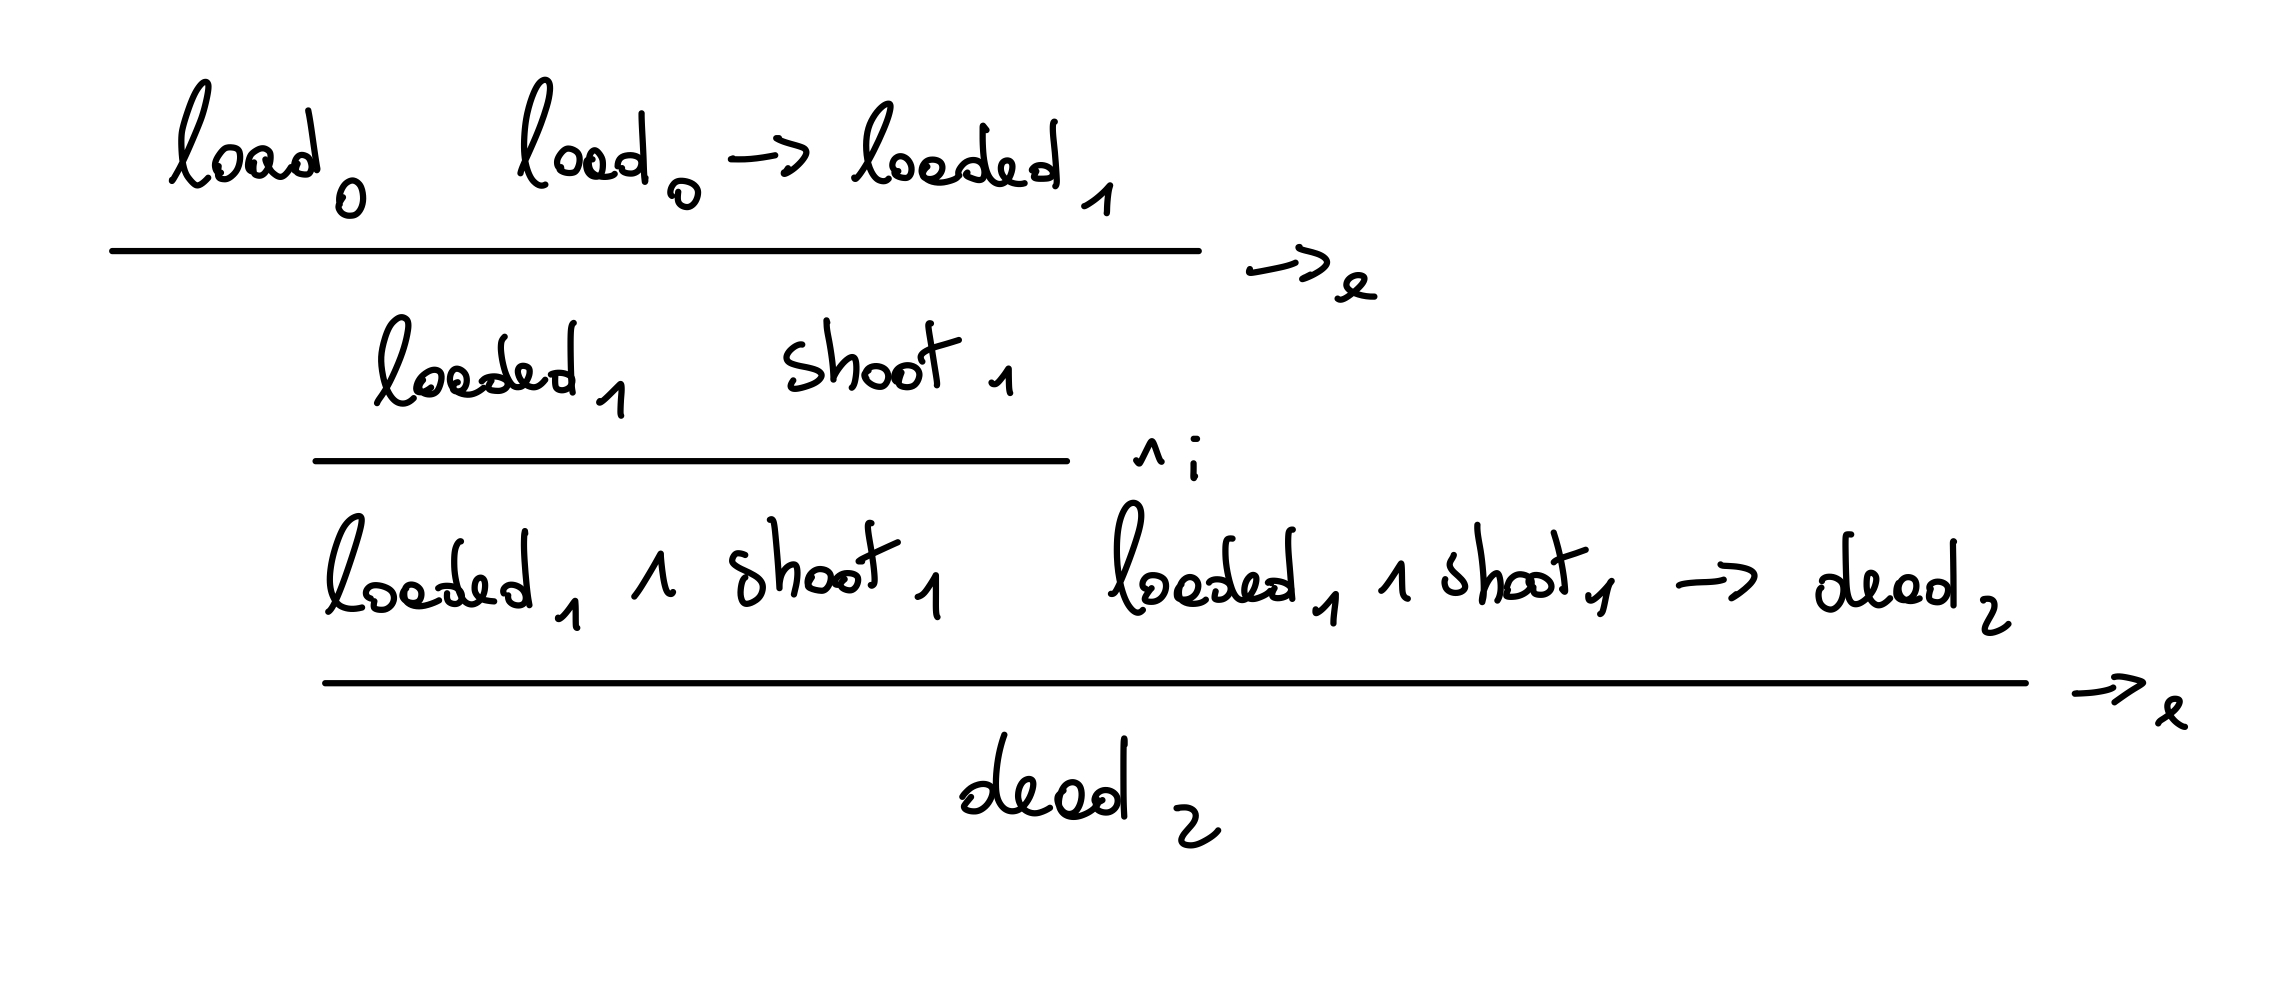
\includegraphics[width=1\textwidth]{img/ysp1.jpeg}
\end{figure}
\\
What about the following situation?
\begin{align*}
    &\text{load}_t\to \text{loaded}_{t+1}\\
    &\text{unload}_t\to \neg \text{loaded}_{t+1}\\
    &\text{loaded}_t\land \text{shoot}_t\to \text{dead}_{t+1}\\
    &\text{load}_0 \\
    &\text{shoot}_2
\end{align*}
Can we conclude $\text{dead}_3$?\\
No, we can't. There is nothing that tells us $\text{loaded}_1 \implies \text{loaded}_2$. That is, nothing tells us that the gun is not unloaded at time 1.\\
Let's try to fix that. 
\begin{align*}
    &\text{load}_t\to \text{loaded}_{t+1}\\
    &\text{unload}_t\to \neg \text{loaded}_{t+1}\\
    &\text{loaded}_t\land \text{shoot}_t\to \text{dead}_{t+1}\\
    &\text{loaded}_t\land\neg\text{unloaded}_t\to \text{loaded}_{t+1}\\
    &\text{load}_0 \\
    &\text{shoot}_2
\end{align*}
Can we conclude $\text{dead}_3$?\\
No, we can't. The gun could be unloaded at time 1. In logic, all that is not specified is not assumed to be false but is not known. So we would need to explicitly say that the gun is not unloaded at time 1. This would be also needed in all successive time steps $[0,t]$. This is not feasible. The commonsense reasoning aims to support a more reasonable representation using non-monotonic logics.\\
Let KB be the set of axioms of the Yale shooting problem. We want to conclude $\text{dead}_3$ from KB assuming that the gun is not unloaded if not specified. In this case the logic is non-monotonic because the set of consequences is not increasing with the addition of new axioms. In the classical logic if KB $\subseteq$ KB' then KB $\vDash$ $\phi$ implies KB' $\vDash$ $\phi$. That is, we cannot invalidate a conclusion by adding new axioms. In the non-monotonic logic, this is not true. We can invalidate a conclusion by adding new axioms.\\
The \textbf{Circumscription} is a non-monotonic logic that allows to reason with incomplete information. The idea is to assume that the world is as simple as possible. In the Yale shooting problem, we can assume that the gun is not unloaded if not specified. This kind of logic is a combination of \textbf{SAT} and a problem of maximization where we want to maximize the number of conclusion that we can draw from the axioms by reducing them. This is what makes the complexity of the problem raise from the 1° level of the polynomial hierarchy to the 2° level.\\
\begin{defbox}[Circumscription]
Let M be the set of propositions that represent abnormal situations, that is the situations that we want to avoid thus we want to make as false as possible. A truth assignment T is preferred (more normal than) to T' iff for every propositional symbol $p\in M$, $T'(p)=\text{false}\implies T(p)=\text{false}$, that is T is at least as normal as T'. In this case we write $T\leq_M T'$. The models of a set of axioms KB (in Circumscription) are the truth assignments T that satisfy KB $(T\vDash KB)$ such that per every T' that satisfies KB, $T'\leq_M T\implies T\le_M T'$. If $\phi$ is true in every model of KB, we write $KB\vDash_M \phi$ and we say that $\phi$ is a logical consequence of KB.\\
\end{defbox}
Now let's see how to use Circumscription to solve the Yale shooting problem. We want to prove that $\text{dead}_3$ is a logical consequence of the axioms. $M={ab_t | t\in\mathbb{N}}$
\begin{align*}
    &\text{load}_t\to \text{loaded}_{t+1}\\
    &\text{unload}_t\to \neg \text{loaded}_{t+1}\\
    &\text{loaded}_t\land \text{shoot}_t\to \text{dead}_{t+1}\\
    &\text{loaded}_t\land\neg\text{ab}_t\to \text{loaded}_{t+1}\\
    &\text{load}_0 \\
    &\text{shoot}_2
\end{align*}
The models here are completely normal: all the $ab_t$ are false. We can derive that $\text{dead}_3$ (KB $\vDash_M$ $\text{dead}_3$).
\begin{figure}[h]
    \centering
    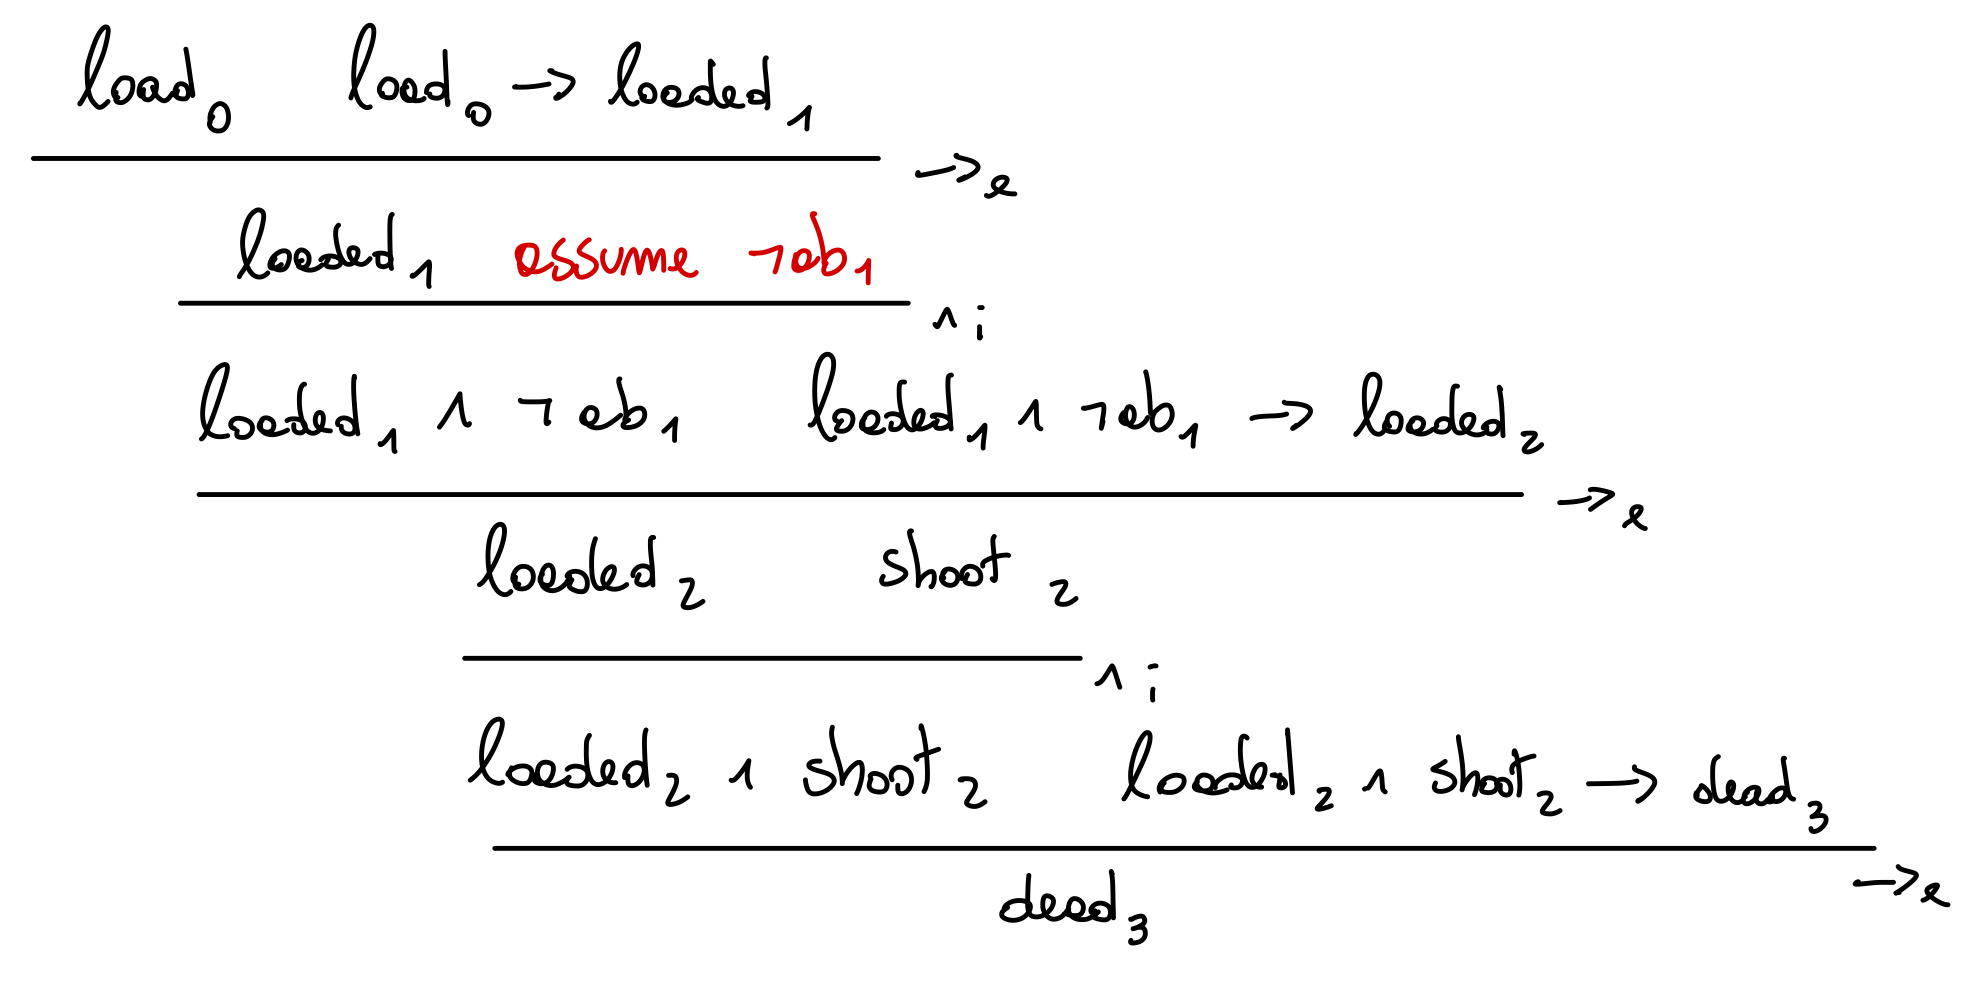
\includegraphics[width=1\textwidth]{img/ysp2.jpeg}
\end{figure}
\\
What about if the gun is unloaded at time 1? 
\begin{align*}
    &\text{load}_t\to \text{loaded}_{t+1}\\
    &\text{unload}_t\to \neg \text{loaded}_{t+1}\\
    &\text{loaded}_t\land \text{shoot}_t\to \text{dead}_{t+1}\\
    &\text{loaded}_t\land\neg\text{ab}_t\to \text{loaded}_{t+1}\\
    &\text{load}_0 \\
    & \textsl{unload}_1 \\
    &\text{shoot}_2
\end{align*}
In this case $\text{unload}_1$ makes $\text{ab}_1$
true in every model of KB to avoid the contradiction $\text{loaded}_2\land \neg\text{loaded}_2$. So we can derive that $\text{dead}_3$ is not a logical consequence of KB.
\begin{figure}[h]
    \centering
    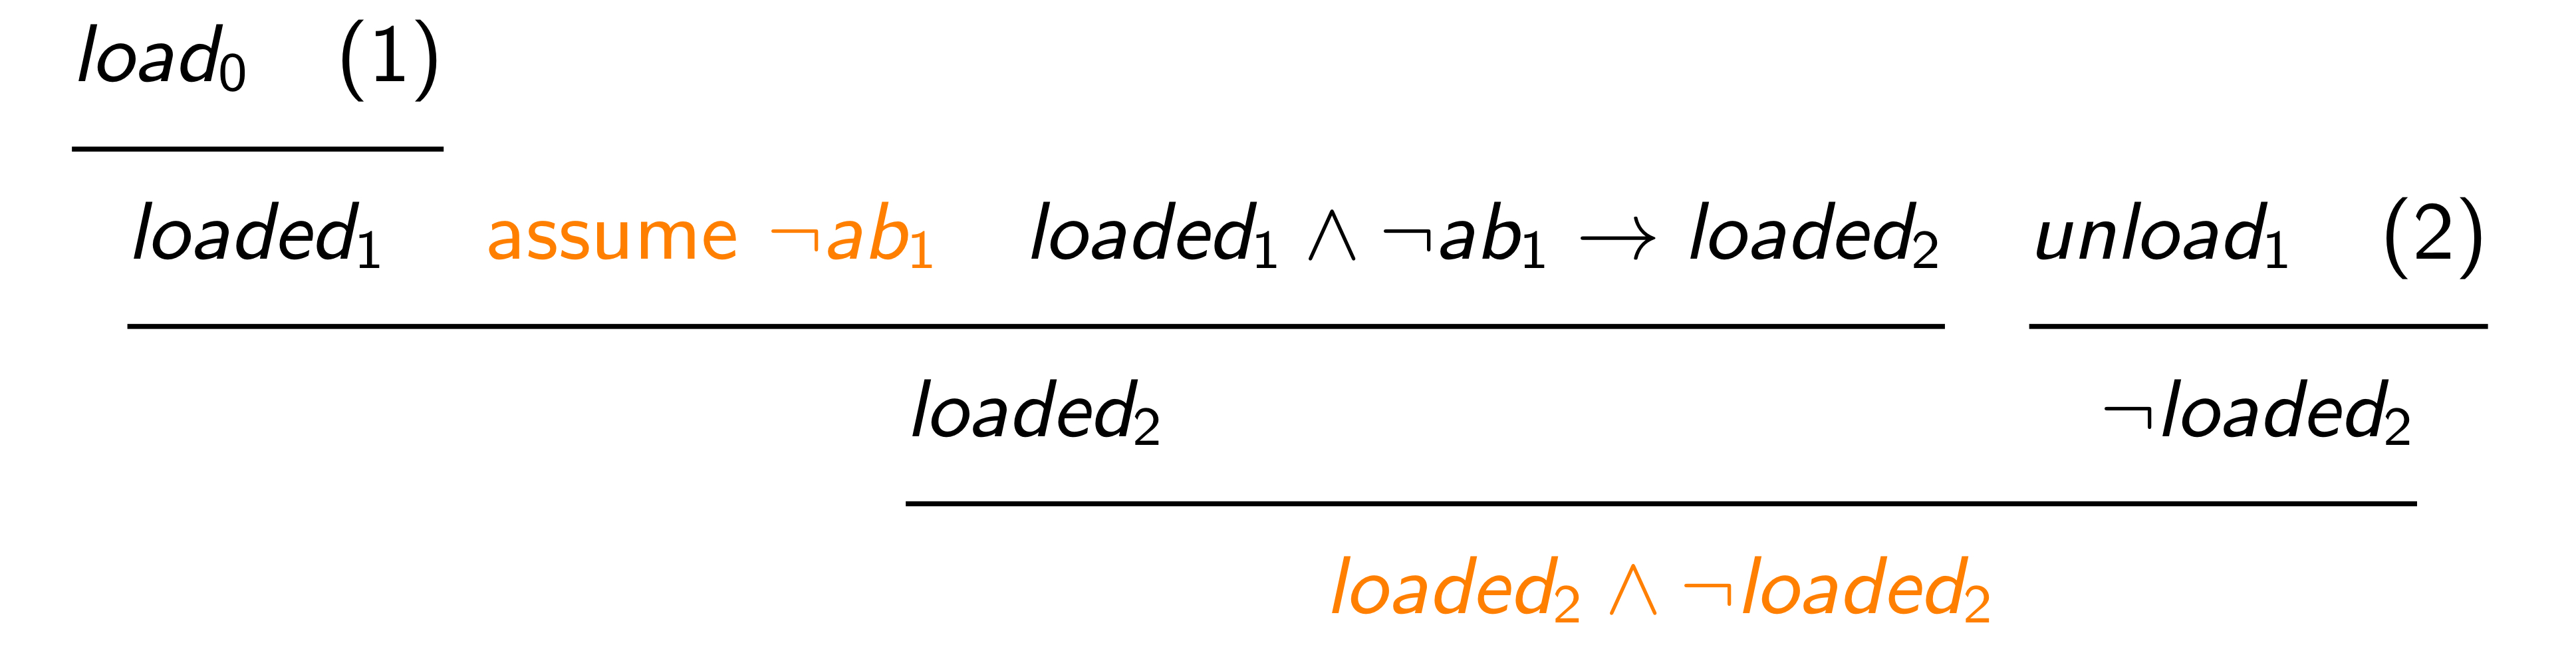
\includegraphics[width=1\textwidth]{img/ysp3.jpeg}
\end{figure}\\
This logic is very flexible, even if we assume $\neg\text{dead}_3$ this makes $\text{ab}_1$ true in every model of KB. So we can derive that $\text{dead}_3$ is not a logical consequence of KB.
\begin{defbox}[Theorem (CIRC SAT and CIRC VALIDITY)]
    Deciding whether a model of KB satisfies $\phi$ is $\Sigma_2\mathbf{P}$-complete.\\
    Deciding whether KB $\vDash_M \phi$ is $\Pi_2\mathbf{P}$-complete.
\end{defbox}
Notice that CIRC SAT $\eqsim$ SAT + minimization of abnormality predicates. As often happens, the complexity of the problem increases when we try to optimize (in this case with minimization) the solution.
The quantified Boolean formulae (QBF) are propositional fragment of the 2° order logic, that is the logic that allows to quantify over the propositional symbols. E.g. $\forall p \exists q.\; \neg p\lor q$ is a QBF. To express the concept of VALIDITY we have something like $\forall p\forall q.\;\neg p\lor p\lor q$. To express satisfiability we have something like $\exists p\exists q.\; p\land q$. To say that a formula in not valid we can say $\forall p\forall q.\; p\lor q$. To say that a formula is not satisfiable we can say $\exists p\exists q.\; p\land \neg p\land q$. In addition to SAT and VALIDITY (1° level) the QBF can express also Circumscription (2° level). For more details refer to the slides. Consequence: The QBF of the form $\exists \vec{x}\forall \vec{y}.\; \phi$ are hard for $\Sigma_2\mathbf{P}$ and the QBF formulae of the form $\forall \vec{x}\exists \vec{y}.\; \phi$ are hard for $\Pi_2\mathbf{P}$. We notice that the number of alternated quantifiers corresponds to the level of the polynomial hierarchy in which the problem is located. Now we give the definition of $QSAT_i$ which is $\Sigma_i\mathbf{P}$-complete.\\
\begin{defbox}[$QSAT_i$]
    Given a QBF with $i$ alternated quantifiers
    \[
\exists p_{1,1} \dots \exists p_{1,n_1} \; \forall p_{2,1} \dots \forall p_{2,n_2} \; \exists p_{3,1} \dots \phi
\]
 more concisely represented as
 \[
\exists \vec{p}_1 \; \forall \vec{p}_2 \; \exists \vec{p}_3 \dots Q \vec{p}_i \; \phi
\]
where $Q$ is $\exists$ if $i$ is odd and $\forall$ if $i$ is even, and where the variables $\vec{p}_1\dots\vec{p}_i$ are all the variables of the formula $\phi$ say if the QBF if true.
\end{defbox}
\begin{defbox}[Theorem]
    $QSAT_i$ is $\Sigma_i\mathbf{P}$-complete.
\end{defbox}
\begin{proof}
omitted
\end{proof}
\begin{defbox}[Theorem]
    CIRC SAT is $\Sigma_2\mathbf{P}$-complete. That is, the problem of deciding whether a formula $\phi$ is true in a model of KB (in the Circumscription logic) is $\Sigma_2\mathbf{P}$-complete.
\end{defbox}
\begin{proof}
    By reduction from $QSAT_2$. Omitted.
\end{proof}
\begin{defbox}
    STRATEGIC COMPANIES is $\Sigma_2\mathbf{P}$-complete.
\end{defbox}
\begin{proof}
    By reduction from $QSAT_2$. Omitted.
\end{proof}
We know that every level of the polynomial hierarchy has same problems that are complete for that level. We don't know if there are problems that are complete for the whole polynomial hierarchy. Is set of all the QBF formulae complete for the whole polynomial hierarchy? Even if seams reasonable to think so the answer is no. Actually it's \textbf{PSPACE}-complete. If we discovered the existence of a problem that is complete for the whole polynomial hierarchy we would have same big consequences.
\begin{defbox}[Theorem 17.11]
    If there was a \textbf{PH}-complete problem, then the polynomial hierarchy would collapse to some finite level.
\end{defbox}
\begin{proof}
Suppose that $L$ is \textbf{PH}-complete. Since $L \in \textbf{PH}$, there is an $i \geq 0$ such that $L \in \Sigma_i\mathbf{P}$. But any language $L' \in \Sigma_{i+1}\mathbf{P}$ reduces to $L$. Since all levels of the polynomial hierarchy are closed under reductions, this means that $L' \in \Sigma_i\mathbf{P}$, and hence $\Sigma_i\mathbf{P} = \Sigma_{i+1}\mathbf{P}$.
\end{proof}
\begin{defbox}[Proposition]
    $\textbf{PH}\subseteq\textbf{PSPACE}$
\end{defbox}
But is $\mathbf{PH} = \mathbf{PSPACE}$? This is an open and intriguing question. However, notice this curious fact:
\begin{defbox}[Corollary]
 If $\mathbf{PH} = \mathbf{PSPACE}$ then by Theorem 17.11 $\mathbf{PH}$ has complete problems ($\mathbf{PSPACE}$ has), and thus the polynomial hierarchy collapses.
\end{defbox}
\begin{defbox}[Definition]
    QSAT is the problem of deciding whether a QBF is true. 
\end{defbox}
\begin{defbox}[Theorem]
    QSAT is \textbf{PSPACE}-complete.
\end{defbox}
\begin{proof}
    Omitted.
\end{proof}

\subsection{Exercise}
\subsubsection{Exercise 1}
Tell if there exist a reduction between the following problems:
\begin{itemize}
    \item $\mathbf{QSAT_2 \; to \; QSAT_4}$\\
    Yes, because $QSAT_4$ is $\Sigma_4\mathbf{P}$-complete and since $QSAT_2\in\Sigma_2\mathbf{P}\subseteq\Sigma_4\mathbf{P}$
    \item $\mathbf{QSAT_4 \; to \; QSAT_2}$\\
    We don't know and if it were the case the polynomial hierarchy would collapse to the 2° level.
    \item $\mathbf{QSAT_i \; to \; \overline{QSAT_i}}$\\
    We don't know and if it were the case we would have that $\Sigma_i\mathbf{P}=\Pi_i\mathbf{P}$ and the polynomial hierarchy would collapse to the $i$th level.
    Same for the other way around.
    \item $\mathbf{CLIQUE \; to \; QSAT_1}$\\
    Yes, because $QSAT_1$ is $\Sigma_1\mathbf{P}$-complete and since $CLIQUE$ is \textbf{NP}-complete and $\textbf{NP}=\Sigma_1\mathbf{P}$ they are complete for the same class. Same for the other way around.
    \item $\mathbf{CLIQUE \; to \; QSAT_2}$\\
    Yes, because $QSAT_2$ is $\Sigma_2\mathbf{P}$-complete, $CLIQUE$ is $\Sigma_1\mathbf{P}$-complete and we know that $\Sigma_1\mathbf{P}\subseteq\Sigma_2\mathbf{P}$ 
    \item $\mathbf{QSAT_2 \; to \; CLIQUE}$\\
    We don't know and if it were the case the polynomial hierarchy would collapse to the 1° level.
    \item $\mathbf{CLIQUE \; to \; \overline{QSAT_1}}$\\
    We don't know and if it were the case we would have that $\Sigma_1\mathbf{P}=\Pi_1\mathbf{P}$ and the polynomial hierarchy would collapse to the 1° level. Same for the other way around.
    \item $\mathbf{CLIQUE \; to \; \overline{QSAT_2}}$\\
    Yes, because $CLIQUE$ is $\Sigma_1\mathbf{P}$-complete, $\overline{QSAT_2}$ is $\Pi_2\mathbf{P}$-complete and we know that $\Sigma_1\mathbf{P}\subseteq\Pi_2\mathbf{P}$.
    \item $\mathbf{ \overline{QSAT_2}\; to \;CLIQUE }$\\
    We don't know and if it were the case we would have that $\Sigma_1\mathbf{P}=\Pi_2\mathbf{P}$ and the polynomial hierarchy would collapse to the 1° level.
    \item $\mathbf{SAT-UNSAT \; to \; QSAT_3}$\\
    Yes, because SAT-UNSAT is \textbf{DP}-complete and $QSAT_3$ is $\Sigma_3\mathbf{P}$-complete. We know that $\textbf{DP}\subseteq\Delta_2\mathbf{P}\subseteq\Sigma_3\mathbf{P}$.
    \item $\mathbf{ QSAT_3\; to \;SAT-UNSAT }$\\
    We don't know and if it were the case we would have that $\Sigma_3\mathbf{P}=\textbf{DP}$ and the polynomial hierarchy would collapse \textbf{at least} to the 2° level. We don't know if the polynomial hierarchy would collapse to the 1° level.
    \item $\mathbf{SAT-UNSAT \; to \; \overline{QSAT_3}}$\\
    Yes, because SAT-UNSAT is \textbf{DP}-complete and $\overline{QSAT_3}$ is $\Pi_3\mathbf{P}$-complete. We know that $\textbf{DP}\subseteq\Delta_2\mathbf{P}\subseteq\Pi_3\mathbf{P}$.
    \item $\mathbf{ \overline{QSAT_3}\; to \;SAT-UNSAT }$\\
    We don't know and if it were the case we would have that $\Pi_3\mathbf{P}=\textbf{DP}$ and the polynomial hierarchy would collapse \textbf{at least} to the 2° level. We don't know if the polynomial hierarchy would collapse to the 1° level.
\end{itemize}
\subsubsection{Exercise 2}
Let's suppose that all the levels of the polynomial hierarchy are distinct. For which $i$ the reduction exists?
\begin{itemize}
    \item $\mathbf{from \; QSAT_i \; to \; QSAT_{i+1}}$\\
    It's true for all $i$. Would be true even without the assumption of distinct levels.
    \item $\mathbf{from \; QSAT_i \; to \; \overline{QSAT_{i+1}}}$\\
    It's true for all $i$. Would be true even without the assumption of distinct levels.
    \item $\mathbf{from \; QSAT_i \; to \; \overline{QSAT_i}}$\\
    It's false for all $i$. Otherwise the hierarchy would collapse to the $i$th level and that would be a contradiction.
    \item $\mathbf{from \; \overline{QSAT_i} \; to \; QSAT_{i+1}}$\\
    It's true for all $i$. Would be true even without the assumption of distinct levels.
    \item $\mathbf{from \; QSAT_i \; to \; TSP(D)}$\\
    It's true only for $i=1$.
    \item $\mathbf{from \; QSAT_i \; to \; VALIDITY}$\\
    Notice that $QSAT_0$ is not a real problem because it would not have any quantifier so it would not be a QBF. So there is no reduction because otherwise the hierarchy would collapse to the 1° level and that would be a contradiction. So it's false for all $i$.
    \item $\mathbf{from \; VALIDITY \; to \;QSAT_i }$\\
    it's true for all $i\ge 2$. For $i=1$ we would have that the hierarchy would collapse to the 1° level and that would be a contradiction.
\end{itemize}
\subsubsection{Exercise 3}
Let's suppose that \textbf{PH} as no complete problems. Is there a reduction between the following problems?
\begin{itemize}
    \item $\mathbf{QSAT_1 \; to \; QSAT_4}$\\
    Yes.
    \item $\mathbf{QSAT_4 \; to \; QSAT_1}$\\
    No, otherwise the polynomial hierarchy would collapse to the 1° level. 
    \item $\mathbf{QSAT_i \; to \; \overline{QSAT_i}}$\\
    No, for both directions. Otherwise the polynomial hierarchy would collapse to the $i$th level.
    \item $\mathbf{CLIQUE \; to \; QSAT_1}$\\
    Yes, because they are both $\Sigma_1\mathbf{P}$-complete. 
    \item $\mathbf{CLIQUE \; to \; CIRC \; SAT}$\\
    Yes, because $CIRC \; SAT$ is $\Sigma_2\mathbf{P}$-complete and $CLIQUE$ is $\Sigma_1\mathbf{P}$-complete. We know that $\Sigma_1\mathbf{P}\subseteq\Sigma_2\mathbf{P}$.
    \item $\mathbf{ CIRC \; SAT\; to \;CLIQUE }$\\
    No, otherwise the polynomial hierarchy would collapse to the 1° level.
    \item $\mathbf{ \overline{QSAT_1}\; to \; CLIQUE}$\\
    No , because CLIQUE is $\Sigma_1\mathbf{P}$-complete and $\overline{QSAT_1}$ is $\Pi_1\mathbf{P}$-complete. Otherwise the polynomial hierarchy would collapse to the 1° level.
    \item $\mathbf{CLIQUE \; to \; \overline{STRATEGIC \; COMPANIES}}$\\
    Yes, because $CLIQUE$ is $\Sigma_1\mathbf{P}$-complete and $\overline{STRATEGIC \; COMPANIES}$ is $\Pi_2\mathbf{P}$-complete. We know that $\Sigma_1\mathbf{P}\subseteq\Pi_2\mathbf{P}$.
    \item $\mathbf{\overline{STRATEGIC \; COMPANIES} \; to \;CLIQUE }$\\
    No, otherwise the polynomial hierarchy would collapse to the 1° level.
    \item $\mathbf{QSAT \; to \; QSAT_3}$\\
    No, because $QSAT$ is \textbf{PSPACE}-complete and $QSAT_3$ is $\Sigma_3\mathbf{P}$-complete. Otherwise the polynomial hierarchy would collapse to the 3° level.
    \item $\mathbf{QSAT_3 \; to \;QSAT }$\\
    Yes, because $QSAT$ is \textbf{PSPACE}-complete and $QSAT_3$ is $\Sigma_3\mathbf{P}$-complete. We know that $\Sigma_3\mathbf{P}\subseteq\textbf{PSPACE}$.
    \item $\mathbf{QSAT \; to \; \overline{HAMILTON \; PATH}}$\\
    No, because $QSAT$ is \textbf{PSPACE}-complete and $\overline{HAMILTON \; PATH}$ is $\Pi_2\mathbf{P}$-complete. Otherwise the polynomial hierarchy would collapse to the 2° level.
    \item $\mathbf{\overline{HAMILTON \; PATH} \; to \; QSAT}$\\
    Yes, because $QSAT$ is \textbf{PSPACE}-complete and $\overline{HAMILTON \; PATH}$ is $\Pi_2\mathbf{P}$-complete. We know that $\Pi_2\mathbf{P}\subseteq\textbf{PSPACE}$.
\end{itemize}



\section{Database queries}
\subsection{Complexity measures}
There are different complexity measures for the queries:
\textbf{Combined Complexity} where both the queries and the database are part of the input; \textbf{Data complexity} where only the database is part of the input (we consider the size of the query negligible); \textbf{Expression complexity} where only the query is part of the input (given a database we want to analyze what happens what happens as the query complexity increases)
\begin{defbox}[Theorem]
    \begin{itemize}
        \item Combined complexity: \textbf{PSPACE}-complete
        \item Expression complexity: \textbf{PSPACE}-complete
        \item Data complexity: \textbf{L}-complete $(\textbf{L}\subseteq \textbf{P})$
    \end{itemize}
\end{defbox}
The \textbf{congiuntive queries} are queries without unions and negations. When we only use this type of queries, the complexity is: 
\begin{itemize}
        \item Combined complexity: \textbf{NP}-complete
        \item Expression complexity: \textbf{NP}-complete
        \item Data complexity: $\textbf{AC}_0-complete(\textbf{AC}_0\subseteq\textbf{L}\subseteq \textbf{P})$
\end{itemize}


\section{Games}
In mathematical terms a game is a graph, often a tree. The nodes are similar to the configurations of a turing machine, and he edges (the possibile moves of a player) are similar to the transitions of a nondeterministic turing machine. 
Tris Example:
\begin{figure}[h]
    \centering
    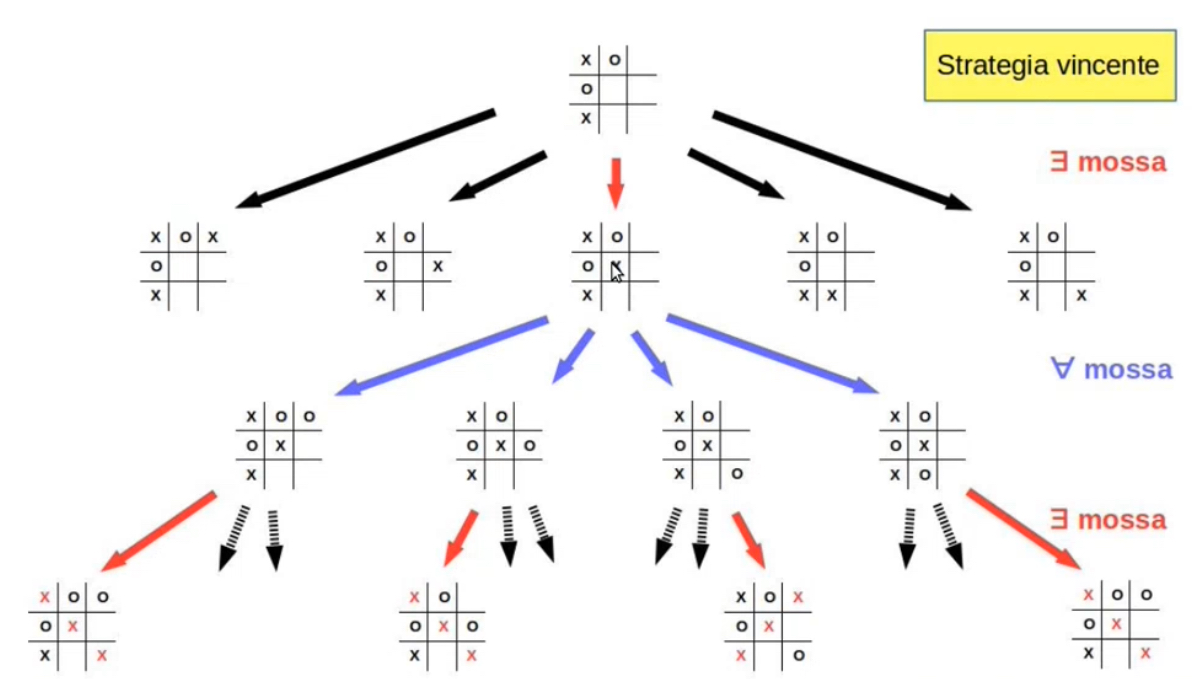
\includegraphics[width=1\textwidth]{img/tris.jpeg}
    \caption{Tris game}
\end{figure}
\\
It is quite clear that there is an analogy between the study of the games strategies and the quantifiers alternation of QBF which characterize the PSPACE complexity classe.
Games with a constant umber of configurations like tris are not very interesting, but e.g the game of chess which has a fixed number of configurations is very interesting because the number of configurations is comparable to the number of atoms in the universe. We still don't know if there is a winning strategy for the first player or not. In the complexity theory we are more interested in games with a variable number of configurations. An in interesting aspect is: what is a solution?It must represent in a compact way the winning strategy of a player. That is, what to do in a exponential number of possibile situations. Let's consider the game of Geography. In this game the first player must say the name of a city, the second player must say the name of a city that starts with the last letter of the first city. The game ends when a player cannot find a city. A possibile generalization of this game could be a graph $G=(V,E)$ where the nodes are the cities and the edges are the connections between them. If $(x,y)\in E$ then the player can say $y$ if the previous player said $x$.
\begin{defbox}[Theorem]
    GEOGRAPHY is \textbf{PSPACE}-complete.
\end{defbox} 
Another interesting game is GO. In this game there is a board of $191times 19$, and the two players alternately place black and white pieces on the board. When a pies is surrounded by the pieces of the other player, it is removed from the board. The game ends when no player can place any more pieces on the board. The winner is the player with the most pieces on the board. 
\begin{figure}[h]
    \centering
    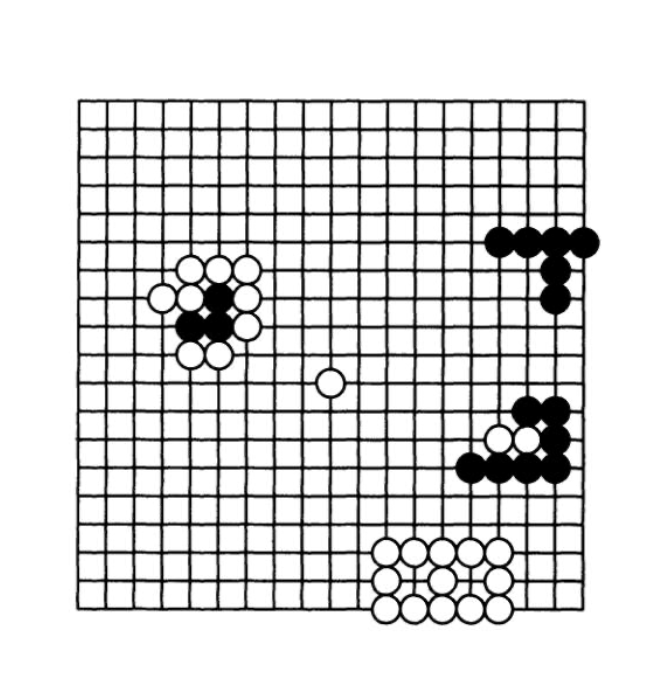
\includegraphics[width=1\textwidth]{img/go.png}
    \caption{GO game}
\end{figure}
\\
To generalize this game we can consider a board of $n\times n$ and decide whether the first player has a winning strategy.
\begin{defbox}[Theorem]
    GO is \textbf{PSPACE}-complete.
\end{defbox}
\subsection{Exercises}
\textbf{Geography can be reduced to the problem of finding a truth assignment in a QBF $\phi$?} Yes, because there is a reduction from Geography to QSAT. That is, given any instance of Geography, we can construct $\phi$ such that is satisfiable if and only if the first player has a winning strategy. I also know that $\phi$ can be constructed in logarithmic space since there is a reduction.
\textbf{If yes, tell if there exists a unique $k$ that upper-bounds the alternation of quantifiers in $\phi$ for every instance of Geography.} We don't know and if it were the case then the polynomial hierarchy and PSPACE would collapse to $\Sigma_k\mathbf{P}$.


\section{Cryptography}
The cryptographic functions to encrypt and decrypt messages used today are not scure in the absolute sense. They are based on mathematical functions that are easy to compute in one direction, but hard to compute in the other direction. It could be possibile to break the security even without knowing the key. The security of the system is based on the fact that finding the key is computationally infeasible in a reasonable time. The problem of breaking the cipher belong to a complexity class that is strictly bigger than P. Encrypting and decrypting a message are not decision problems, so they belong to a specific complexity class. The existing condition of the cryptographic function is not related to the $P\not= NP$ hypothesis but on the hypothesis that $P\not= UP$, where $UP$ is a subclass of $NP$.
\subsection{Function problems}
Remember that a decision problem $L$ is in \textbf{NP} iff there exist a relation $R_L$ polynomially balanced and decidable in polynomial time such that:
$$
L=\{x\;|\; \exists y such that (x,y)\in R_L\}
$$
The certificate $y$ represents a solution to the instance $x$.
\begin{defbox}[Function problme]
    Given an instance $x$ of $L$, finding a string $y$ such that $(x,y)\in R_L$ is called a \textbf{function problem}. If there is no solution, the function returns \dquote{no}.
\end{defbox}
\begin{defbox}[FNP]
    The class of function problems FL such that $L\in NP$ is called \textbf{FNP}. 
\end{defbox}
\begin{defbox}[FP]
    The class of function problems FL such that $L\in P$ is called \textbf{FP}.
\end{defbox}
Clearly, $FP\subseteq FNP$. With the use of oracles, we can define the functional class of $PH$.
To reduce a functional problem $A$ to a functional problem $B$, it's not enough to transform the instance of $A$ into an instance of $B$. We also need to transform the solution for $B$ into a solution for $A$. 
\begin{defbox}[Reduction for function problems]
    A function problem $A$ is \textbf{reducible} to a function problem $B$ if there exist two functions $R$ and $S$ such that:
    \begin{itemize}
        \item $R$ and $S$ are computable in logarithmic space
        \item if $x$ is an instance of $A$, then $R(x)$ is an instance of $B$
        \item the answer to $X$ is \dquote{no} iff the answer to $R(x)$ is \dquote{no}
        \item if $y$ is a solution for $R(x)$, then $S(y)$ is a solution for $x$
    \end{itemize}
\end{defbox}
\begin{defbox}[Completeness for function problems]
    A problem $A$ is \textbf{complete} for a class of function problems $FC$ iff:
    \begin{itemize}
        \item $A$ is in $FC$
        \item for every problem $B$ in $FC$, $B$ is reducible to $A$
    \end{itemize}
\end{defbox}
One problem that is complete for \textbf{FNP} is \textbf{FSAT}.
That is the problem of finding a truth assignment that satisfies a boolean formula.

\newpage
\subsection{\textcolor{red}{FSAT and SAT}}
\begin{defbox}[\textcolor{red}{Proposition (Relation between FSAT and SAT)}]
    \textbf{FSAT} can be solved in polynomial time if and only if \textbf{SAT} can be solved in polynomial time.
\end{defbox}
\begin{proof}
Given a deterministic turing machine $M$ that solves \textbf{FSAT} in polynomial time, we can construct a deterministic turing machine $M'$ that solves \textbf{SAT} in polynomial time. The machine $M'$ will be just like $M$, except that every time $M$ outputs a solution, $M'$ will output \dquote{yes}. We just need to ignore the solution. Now let's prove the other direction. Given a deterministic algorithm $A$ that solves \textbf{SAT} in polynomial time, we can construct a deterministic algorithm $A'$ that solves \textbf{FSAT} in polynomial time that works as follows:

\begin{algorithm}
\caption{Truth Assignment Algorithm}
\begin{algorithmic}[1]
\State \textbf{Input:} $\phi(x_1, \ldots, x_n)$
\State \textbf{Output:} truth assignment $T$ or \texttt{"no"}
\\
\If{$A(\phi(x_1, \ldots, x_n)) = \texttt{"no"}$}
    \State \Return \texttt{"no"}
\EndIf
\For{$i = 1$,\dots,$n$}
    \If{$A(\phi(T[1], \ldots, T[i-1], \text{true}, x_{i+1}, \ldots, x_n)) = \texttt{"yes"}$}
        \State $T[i] = \text{true}$
    \Else
        \State $T[i] = \text{false}$
    \EndIf
\EndFor
\State \Return $T$
\end{algorithmic}
\end{algorithm}
\end{proof}
\begin{defbox}[Theorem]
    $$\textbf{FP}=\textbf{FNP} \iff \textbf{P}=\textbf{NP}$$
\end{defbox}
\begin{proof}
    If $\textbf{P}=\textbf{NP}$ then the function problems associated to \textbf{P} and \textbf{NP} are the same. So, $\textbf{FP}=\textbf{FNP}$.
    If $\textbf{FP}=\textbf{FNP}$, then \textbf{FSAT} can be solved deterministically in polynomial time. Then for what we demonstrated before, \textbf{SAT} can be solved in deterministic polynomial time. Sine this means that an \textbf{NP}-complete problem is in \textbf{P}, then \textbf{P}=\textbf{NP}. 
\end{proof}

\newpage
\subsection{One-way functions in cryptography}


\section{Above PSPACE}
\subsection{\textcolor{red}{Theorem 20.1}}
\begin{defbox}[\textcolor{red}{Theorem 20.1}]
If \textbf{P}=\textbf{NP} then \textbf{EXP}=\textbf{NEXP}    
\end{defbox}
\begin{proof}
    Let $L\in\textbf{NEXP}$, by definition there exist a nondeterministic TM $N$ that decides $L$ in time $2^{n^k}$.
    Let $L'$ be a langue that enlarges the instances of $L$ exponentially with a new symbol $\sqcap$ called semi-blank.
    $$L' = \left\{ x \sqcap^{2^{|x|^k} - |x|} \;\middle|\; x \in L \right\}$$   
    The semi-blanks enlarge every $x$ to $2^{|x|^k}$ characters. Let first show that $L'\in \textsl{NP}$ using a nondeterministic TM $N'$ obtained from $N$. $N'$ first checks that the input $y$ is well formed, that is $x\sqcap^{2^{|x|^k}}-|x|$ where $x$ does not contain $\sqcap$ (otherwise rejects), then simulates $N$ using $\sqcap$ as it would be $\sqcup$. $N'$ runs in polynomial time thanks to the enlargement of $x$. Since $L'\in \textsl{NP}$ and for hypothesis we have P=NP, we have $L'\in\textsl{P}$. So there must exist a deterministic TM $M'$ that decides $L'$ in polynomial time $n^l$. Then we construct a deterministic TM $M$ based on $M'$ that decides $L$ in exponential time. This will prove that $L\in\textsl{EXP}$ ending the proof. $M$ extends $x$ with $\sqcap$ until it reaches length $2^{|x|^k}$, then executes the instructions of $M'$ on the input. The time required is indeed exponential since the phase 1 takes $O(p(|x|)\cdot2^{|x|^k})=O(2^{|x|^{k+j}})$ for some $j$ where $p$ is the polynomial time require to manipulate the counters and the phase 2 takes $(2^{|x|^k})^l = O(2^{|x|^k+l})$. 
\end{proof}
\section{Summary of problems complexity}
\begin{itemize}
    \item 2-SAT is P-complete
    \item PRIMES $\in$ P
    \item MAX-FLOW is P-complete
    \item SAT is NP-complete
    \item 3-SAT is NP-complete
    \item MAX2SAT is NP-complete
    \item INDEPENDENT SET is NP-complete
    \item CLIQUE is NP-complete
    \item NODE COVER is NP-complete
    \item SET COVER is NP-complete
    \item HAMILTON PATH is NP-complete
    \item TSP(D) is NP-complete
    \item 3-COL is NP-complete
    \item TRIPARTITE MATCHING is NP-complete
    \item KNAPSACK is NP-complete
    \item VALIDITY is coNP-complete
    \item $\overline{\text{HAMILTON PATH}}$ is coNP-complete
    \item $\overline{\text{TSP(D)}}$ is coNP-complete
    \item Schönfinkel-Bernays SAT is coNP-complete
    \item $\textsl{QSAT}_i$ is $\Sigma_iP$-complete
    \item $\overline{\textsl{QSAT}_i}$ is $\Pi_iP$-complete
    \item SAT-UNSAT is DP-complete
    \item STRATEGIC COMPANIES is $\Sigma_2P$-complete
    \item $\overline{\text{STRATEGIC COMPANIES}}$ is $\Pi_2P$-complete
    \item GEOGRAPHY is PSPACE-complete
\end{itemize}
\end{document}